%!TEX encoding = UTF-8 Unicode
\documentclass[a4paper,12pt]{book}
%\usepackage[top=3.5cm,right=3cm,bottom=4cm,left=3cm]{geometry}  
\usepackage{amsmath}
 \usepackage[marginal,stable,bottom]{footmisc}     % for footnotes: marginal --> the same margins as text, 
                                                                                  %                       stable--> ?
                                                                                  %                       bottom --> starting the footnotes at a fixed place at the bottom of the page.
 
\usepackage{perpage}                                             % for footnotes: starting from 1 perpage
\MakePerPage{footnote}
\usepackage{cite}                                                     % for collecting citations: [1,2,3,4] --> [1-4]
\usepackage{setspace}                                            % for switching between double/single space in document
\allowdisplaybreaks                                                    % breaking the lines&pages when needed for the style.
\usepackage{parskip}                                               % ? 

%\relpenalty=9999                                            % show the neccessity of breaks for lines, changing the number to 10000 cause no break in lines.
%\binoppenalty=9999
%%%%%%%%%% by me
\usepackage{textcomp}
\usepackage{amssymb}
%%%%%%%%%%
\usepackage{xecolour}
\usepackage{url}
\usepackage{mathtools}
\usepackage{amsmath}
\usepackage{makeidx}
\usepackage{verbatim}
\usepackage[colorlinks,linkcolor=blue,citecolor=blue]{hyperref}
\usepackage{graphicx}
\usepackage{ifthen}

 \parindent0pt


\makeatletter
\pdfstringdefDisableCommands{%
\let\lr\@firstofone
}
\makeatother
% ----------------------------------------------------------------------------
\usepackage{xepersian}

\usepackage[Lenny]{fncychap}

\settextfont[Scale=1.07]{XB Niloofar}
\setlatintextfont[Scale=1.05]{Times New Roman} 
\setdigitfont[Scale=1.05]{XB Niloofar} 
% \setdigitfont[Scale=1.05]{Yas} 
% قلم برای اعداد به صورت فارسی با صفر توخالی، در صورتی که بخواهیم اعداد انگلیسی نوشته شوند این خط را غیر فعال می‌کنیم.


\defpersianfont\nastaliq[Scale=2.0]{IranNastaliq}
% قلم برای نوشتن تقدیم
\defpersianfont\nastaliqone[Scale=1.0]{IranNastaliq}
% قلم نستعلیق با سایز متناسب با متن در صورت نیاز
\defpersianfont\anotherfont[Scale=1.2]{XP Ziba}
% قلم برای نوشتن تشکر (قلم فانتزی)
\newenvironment{fantezi}
{\anotherfont }


\makeindex


\def\beginto{
\newpage
\begin{RTL}
\begin{Huge}
\nastaliq

\begin{center}
\vspace*{0.15cm}
}

\def\endto{
~
\end{center}
\end{Huge}
\end{RTL}
}

\def\beginthanks{
\newpage

{\centering\Huge{\nastaliqone{
تشکر وقدردانی ~\\
~\\}}}
}

\def\endthanks{
~
}

\def\thanks{
\beginthanks
\input{thanks}
\endthanks
}

\def\startpage{
\newpage
\vspace*{3cm}
\begin{center}

\includegraphics[width=12cm]{besm}
\end{center}
}
\makeatletter
\def\@makechapterhead#1{%
  \vspace*{50\p@}%
  {\parindent \z@ \centering\normalfont
    \ifnum \c@secnumdepth >\m@ne
      \if@mainmatter
        \huge\bfseries \@chapapp\space \tartibi{chapter} 
        \par\nobreak
        \vskip 20\p@
      \fi
    \fi
    \interlinepenalty\@M
    \Huge \bfseries #1\par\nobreak
    \vskip 40\p@
  }}
\def\@makeschapterhead#1{%
  \vspace*{50\p@}%
  {\parindent \z@ \centering
    \normalfont
    \interlinepenalty\@M
    \Huge \bfseries  #1\par\nobreak
    \vskip 40\p@
  }}
\makeatother



\renewcommand\bibname{مراجع}
\def\contentsname{فهرست}

% some extra diffinitions %%%%%%%%%%%%%%%%%
%%%%%%%%%%%%%%%%%%%%%%%%%%%%%

\def\bea{\begin{eqnarray}}
\def\eea{\end{eqnarray}}

\def\ba{\begin{array}}
\def\ea{\end{array}}

\def\ni{\noindent}
\def\nn{\nonumber}

\def\bc{\begin{center}}
\def\ec{\end{center}}

\usepackage{graphicx}
\usepackage[top=3cm,right=2.5cm,bottom=3cm,left=2.5cm]{geometry}  
\usepackage{fancyhdr}
\usepackage{amssymb} %for complicated latex symbols
\usepackage{amsmath}
\pagestyle{plain}
\usepackage[colorlinks,linkcolor=blue,citecolor=blue,pagebackref=false]{hyperref}
\usepackage{xepersian}
\settextfont[Scale=1]{XB Niloofar}
\setlatintextfont[Scale=1]{Times New Roman}
\setdigitfont[Scale=1]{XB Niloofar}

\lhead{\thepage}
\chead{}
\cfoot{}
\renewcommand{\headrulewidth}{0.4pt}
\renewcommand{\footrulewidth}{0.4pt}

\fancypagestyle{fpstyle}{%
\fancyhead{} % get rid of headers
\renewcommand{\headrulewidth}{0pt} % and the line
}
\setlatintextfont[Scale=.9]{Times New Roman}
\graphicspath{{Figs/}}

\newcommand{\fatitle}{بررسی چیدمان کروماتین درون هسته}
\newcommand{\faAuthor}{علی فرنودی}
\newcommand{\fasupervisor}{دکتر محمد رضا اجتهادی}
\newcommand{\fadate}{آبان 1396}
\newcommand{\falevel}{دکتری}
\newcommand{\fadepart}{دانشکده فیزیک}

%\newcommand{\entitle}{ DNA chains entanglement in confined geometries}
%\newcommand{\enAuthor}{Zahra Ahmadian}
%\newcommand{\ensupervisor}{Mohammad Reza Ejtehadi}
%\newcommand{\engdate}{August 2015}
%\newcommand{\enlevel}{Master of Science}
%\newcommand{\enDep}{Physics Department}

%\newcommand{\momtahenin}{دکتر سامان مقیمی عراقی }
%\newcommand{\momtahenou}{دکتر عباس  علی صابری}
\usepackage{perpage} %the perpage package
\usepackage{amsmath}
\MakePerPage{footnote} %the perpage package command



\begin{document}

\cleardoublepage
\pagenumbering{roman} 

\begin{center}
\thispagestyle{empty}

\includegraphics{Figs/logo} \\
\begin{Large}
دانشگاه صنعتی شریف \\
\fadepart \\ [1cm]
رساله  \falevel \\

\end{Large}
\vskip 3cm
\large{عنوان}  \\ \textbf{\large{\fatitle}}
\vskip 2cm
\large{نگارنده:} \\ \Large{\faAuthor}
\vskip 2cm
\large{استاد راهنما:} \\ \Large{\fasupervisor}
\vskip 2cm
\large{\fadate}
\end{center}


\thispagestyle{empty}
\noindent
\vskip 7cm
\begin{center}

\includegraphics[scale=0.8]{Figs/besm.png}
\end{center}
\thispagestyle{empty}
\noindent
\centerline{\textbf{\large{چکیده}}} \\
در فصل اول این پژوهش مروری بر مطالعات اخیر افراد در مورد ساختار اسکلت سلولی و عوامل دخیل در انتقال نیرو در سلول‌های دارای هسته شده است. فیزیک رفتار مواد ویسکوالاستیک با جزئیات نیز بررسی شده‌. در ادامه‌ی این فصل برخی مطالعات منتخب معرفی شده‌ که در آن از مدل‌های ویسکوالاستیکی برای  مدل‌سازی نتایج آزمایشگاهی رفتار بخش‌های مختلف سلول استفاده شده‌است. در نهایت ساختار کروماتین در هسته‌ی سلول و ماتریس اتصالات کروماتین‌ها درون هسته نیز بررسی شده‌است. همچنین برخی از مدل‌هایی که در ۲-۳ سال گذشته برای توجیه این ساختار و ماتریس اتصالات انتشار یافته نیز مطالعه شده‌است. \\
در فصل دوم طرح پژوهشی توضیح داده شده و در فصل آخر منابع مورد استفاده نامبرده شده‌است.
\\
\\
\textbf{کلمات کلیدی:}
کروماتین، ماتریس اتصالات، ویسکوالاستیک، هسته سلول، شبیه‌سازی دینامیک ملکولی
\textit{}



\tableofcontents
\clearpage
\listoffigures
\clearpage
%\listoftables
\chapter{فصل ۱}
\setRL
\clearpage
\pagenumbering{arabic} 
\section{بررسی اجمالی پژوهش}


نقش فیزیکدانان در علوم زیستی ارائه دیدگاه‌های بدیع برای توصیف پدیده‌های زیستی‌است. به عنوان مثال مواد زیستی اغلب با مدل‌های فیزیک مواد نرم قابل توصیف هستند. $DNA$ یک پروتئین پیچیده‌ی بسیار بلند است که در مورد انسان‌ها طول آن به ۲-۳ متر می‌رسد\cite{Kauffman:1999yu}. قطر $DNA$ حدود ۱ نانومتر است\cite{WATSON:1953fr} و به کمک پروتئین‌های درون هسته بسته بندی و فشرده می‌شود که در این حالت آنرا کروموزوم\LTRfootnote{Chromosome} می‌نامیم. طول کروموزوم‌ها $0.2-20\mu m$ است و تنها هنگام تقسیم سلولی است که دارای نظم هستند و در کنار نسخه‌ی رونوشت‌شان به شکل X‌ با میکروسکوپ نوری قابل مشاهده هستند\cite{CHAFFEY:2003cr}. 

 ساختار کروماتین نقش مهمی در فرآیندهای سلولی دارد زیرا باعث می‌شود رشته‌ی بلند $DNA$ بیش از حد در هم تنیده نشود و برای ساز و کار‌هایی مانند خواندن و نوشتن ژن و ایجاد نسخه رونوشت قابل دسترس باشد\cite{PhysRevLett.120.088101, CHAFFEY:2003fv}. حیات سلول به ساختار کروموزوم وابسته است. در صورتی که هنگام تولید مثل سلول ساختار کروموزوم‌ها دچار اختلال شود باعث مرگ سلول می‌شود. 
 کروماتین‌ها در کنار یکدیگر تقریبا تمام فضای هسته را اشغال می‌کنند. در هسته‌ی سلول‌های انسان ۲۳ جفت کروموزوم وجود دارد که در مجموع ۴۶ کروموزوم در هر سلول قرار گرفته‌است.  به مجموعه‌ی $DNA$، چندین پروتئین، و $RNA$ کروماتین\LTRfootnote{Chromatin} گفته می‌شود. وظیفه‌ی اصلی کروماتین را می‌توان در موارد زیر خلاصه کرد:\\\\
۱-بسته بندی $DNA$ در فضای بسیار چگال\\
۲-مقاوم و آماده‌سازی $DNA$ برای تقسیم سلولی\\
۳-مراقبت از $DNA$ در مقابل آسیب\\
۴-تنظیم $DNA$ برای خوانده شدن ژن و عملیات مربوط به DNA\\

وظیفه‌ی اصلی بسته بندی $DNA$ در کروماتین به عهده‌ی هیستون\LTRfootnote{Histone} است\cite{Hammond:2017sp}. هیستون معمولا در سلول‌های دارای هسته دیده می‌شود.

 برای بررسی ساختار و نحوه‌ی مدیریت این ساختار توسط سلول نیاز به کمی کردن\LTRfootnote{Quantification}  خواص ساختار و دینامیک آن، همکاری فیزیکدانان را ممکن کرده‌است. فیزیکدانان سلول  را یک سیستم خارج از تعادلِ دارای حرکت\LTRfootnote{Dynamic}
می‌دانند که در آن اسکلت سلولی\LTRfootnote{Cytoskeleton} با پلیمریزه\LTRfootnote{Polymerise}(و دی‌پلیمریزه\LTRfootnote{Depolymerise}) شدن به صورت خودساماندهی‌ شده در ساختار‌های منظمی  قرار می‌گیرد که با قوانین فیزیک مواد نرم قابل توصیف است.\cite{Caballero:2015ty} اسکلت سلولی قادر به انتقال نیروهای خارجی به اعضای داخلی هسته است. به عنوان مثال مشاهده‌ شده‌است که هنگامی که سلول بر روی سطوح ناهموار قرار می‌گیرند شکل هسته تغییر می‌کند\cite{Heydari:2017cy}. برای بررسی تاثیر نیروهای خارجی بر هسته‌ی سلول اسکلت سلولی را بیشتر بررسی می‌کنیم.

\subsection{اسکلت سلولی}\label{lab:skeleton}
تمامی سلول‌های موجودات زنده اسکلت سلولی دارند. اسکلت سلولی یک شبکه پیچیده تشکیل شده از رشته‌ها یا فیلامنت‌\LTRfootnote{Filament}ها و لوله‌های نازک یا میکروتیوبول‌\LTRfootnote{Microtubule}هاست که در داخل سیتوپلاسم\LTRfootnote{Cytoplasm} از هسته تا غشای سلول توزیع شده‌است (شکل \ref{fig:wiki-cyto})\cite{hardin2014becker,PhysRevLett.120.068001}. این مجموعه اساس اسکلت سلولی است و بستر اسکلت برون سلولی را ایجاد می‌کند. این شبکه دائما در حال تغییر است و به طور عمومی از ۳ نوع پروتئین (شامل اکتین\LTRfootnote{Actin}) تشکیل شده است. در صورت نیاز سلول، این پروتئین‌ها با سرعت خیلی زیادی پلیمریزه (رشد) یا دیپلیمریزه (تخریب) می‌شوند. ویژگی اصلی اسکلت سلولی، که مورد توجه ماست، قابلیت آن در شکل دادن به سلول و عکس العمل در برابر نیرو‌ی خارجی است به خصوص نیروهایی که از طریق ماتریس برون سلولی\LTRfootnote{Extra-Celluler Matrix ($ECM$)} به سلول منتقل می‌شود\cite{PhysRevLett.120.068001}. مدل‌سازی توزیع نیرو در شبکه‌های پلیمری تصادفی تحت تنش به کمک روش‌های محاسباتی کامپیوتری امکان پذیر است\cite{Heussinger2007}. توزیع نیرو در شبکه‌های جرم و فنر مسئله‌ایست که بیش از یک قرن پیش  ماکسول\LTRfootnote{James Clarck Maxwell} به آن پرداخته است. یکی از نتایج مهم ماکسول این است که در یک شبکه گوی و فنر با افزاریش تعداد همسایه‌های به هم متصل انعطاف شبکه کمتر می‌شود\cite{doi:10.1080/14786446408643668}. در نتیجه اتصالات فیلامنت‌ها باید با چگالی مشخصی باشده تا بتواند ساختار سلول را حفظ کند.




\begin{figure}[h]
\begin{center}
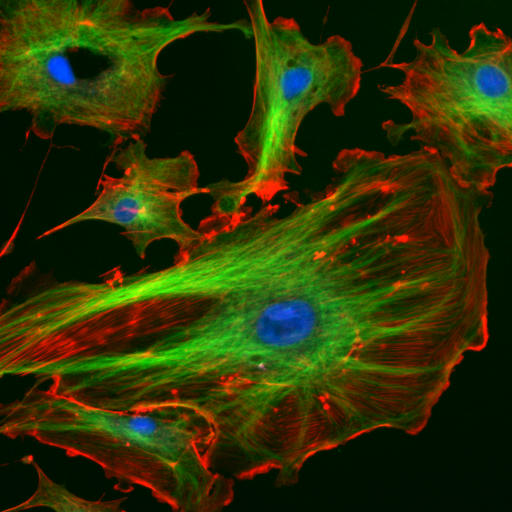
\includegraphics[width=4in]{FluorescentCells}
\caption{
تصویر سلول اندوتلیال (Endothelial) زیر میکروسکوپ نشان داده شده‌است. در این عکس  ناحیه آبی هسته سلول،‌ سبز میکروتیوبول‌ها و قرمز فیلامنت‌های اکتین را نشان می‌دهد.\cite{wiki-cell}
}
\label{fig:wiki-cyto}
\end{center}
\end{figure}
اعضای شبکه اسکلت سلولی با یکدیگر و با پروتئین‌های درون سلول همیشه در حال برهم کنش هستند. موتورهای پروتئینی با انرژی شیمیایی حاصل از آب کافت\LTRfootnote{Hydrolysis} $ATP$\LTRfootnote{Adenosine triphosphate} اعضای این شبکه را تحت تنش\LTRfootnote{Stress} قرار می‌دهد. این انرژی سوخت لازم برای ۲ فرآیند غیر تعادلی اصلی در اسکلت سلولی را فرآهم می‌کند که نقش مهمی در پدیده‌هایی همچون مهاجرت سلول (و برخی باکتری \cite{Mignot853}) بازی می‌کند. پلیمریزه شدن فیلامنت‌ها و برهمکنش موتور‌های پروتئینی با آن‌ها به طور عمومی باعث انقباض اسکلت سلولی می‌شود\cite{Hawkins:2011eu}. 

نقش پلیمریزه شدن توسط اکتین، جریان‌های اکتومایوسینی\LTRfootnote{Actomyosin}، و سامانه‌های میکروتیوبول کینسین\LTRfootnote{Micriotubulekinesin} در حرکت سلول بر روی سطوح ۲ بعدی به خوبی بررسی شده‌است\cite{PhysRevLett.92.078101, refId0, PhysRevE.76.031921}. سلول برای حرکت روی سطوح ۲ بعدی، نقاط اتصال کانونی\LTRfootnote{Focal adhesion point} تشکیل می‌دهد. این نقاط تکیه‌گاه اکتین‌های در حال پلیمریزه شدن هستند که سلول را رو به جهت دلخواه هُل می‌دهند. در سمت مخالف جهت حرکت سلول انقباض اسکلت سلولی حاصل از جریان‌های اکتومایوسینی بر نقاط چسبنده‌ی کانونی غلبه می‌کند و سلول را از سطوح جدا میکند\cite{Hawkins:2011eu} (شکل\ref{fig:migration}).
\begin{figure}[htbp]
\begin{center}
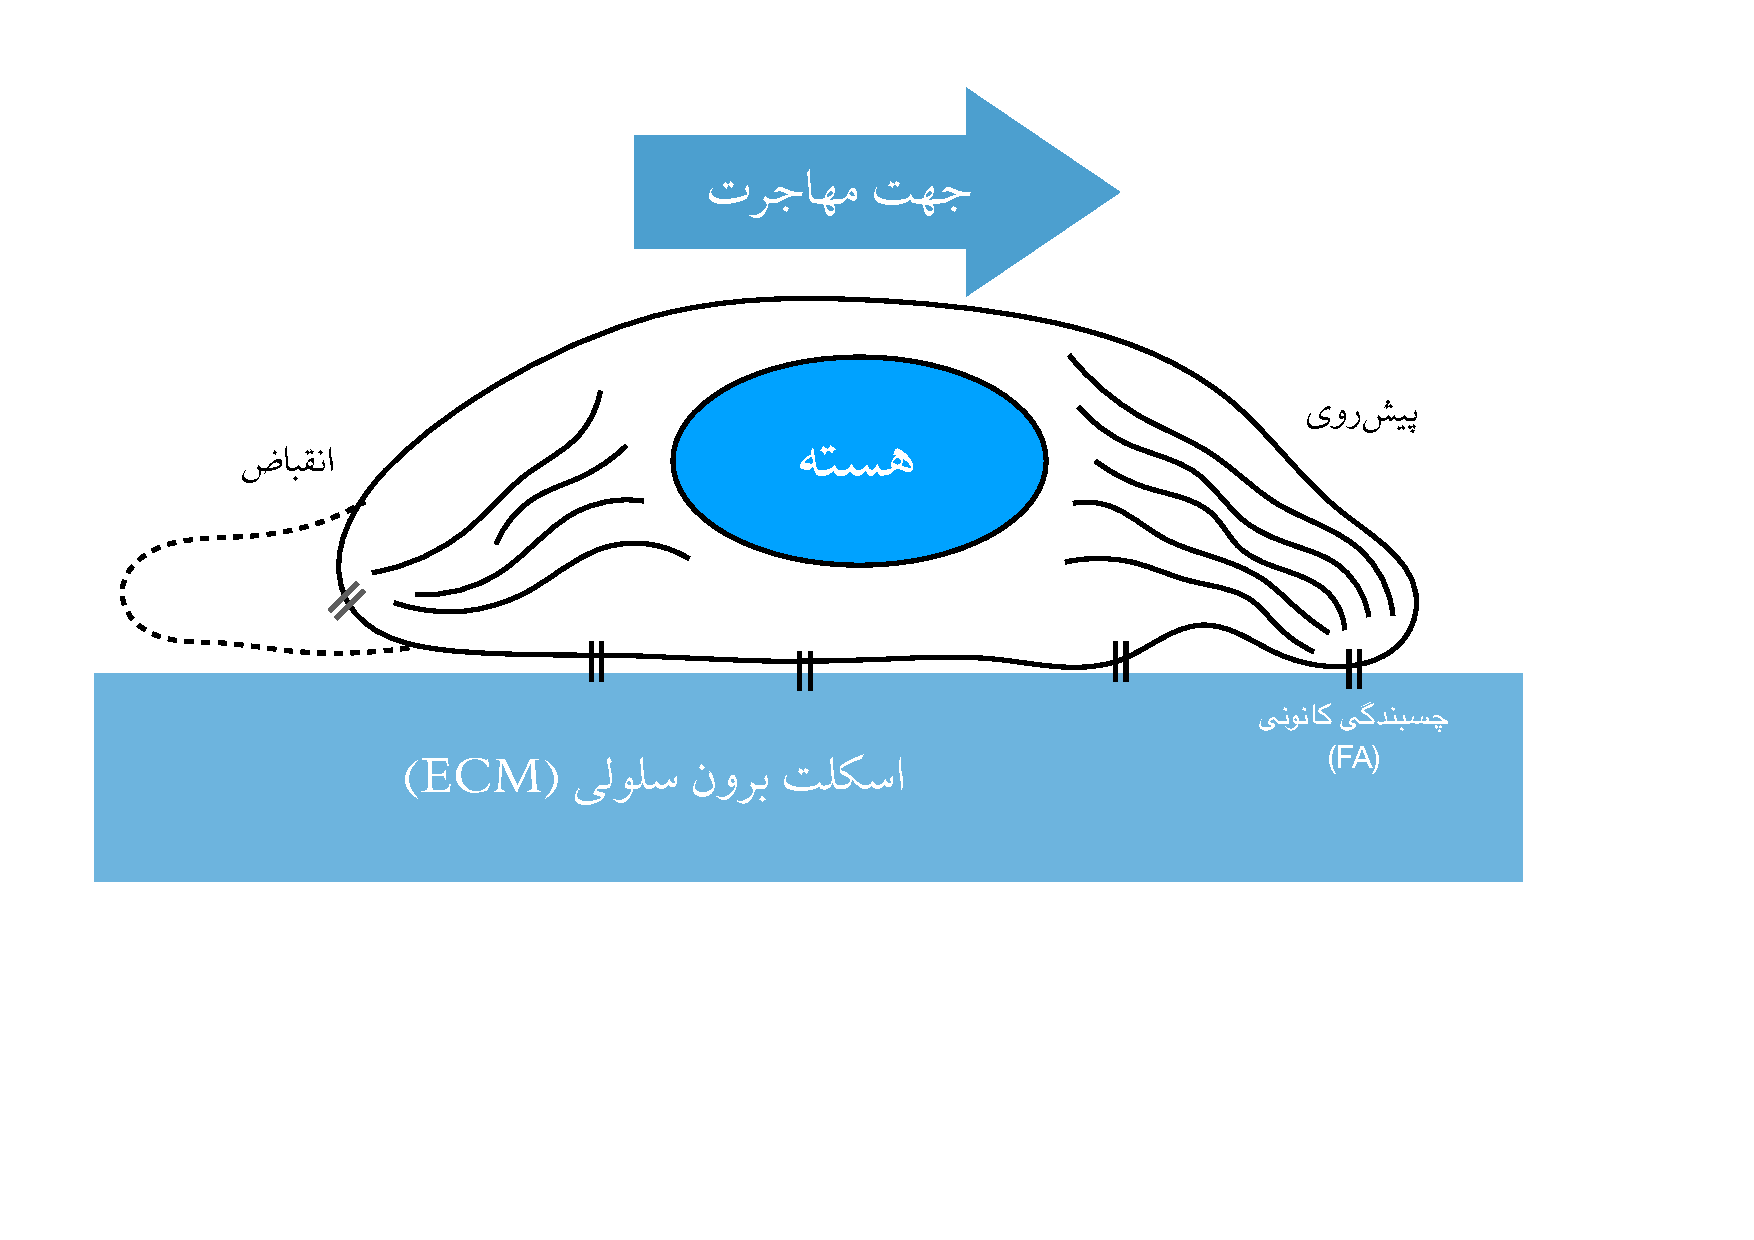
\includegraphics[width=5in]{cell_sketch}
\caption{
دو فرآیند پلیمریزه‌ شدن اکتین در جلو (سمت راست) سلول در محل اتصال کانونی را نشان می‌دهد و شکسته شدن اتصالات کانونی در پشت (سمت چپ) سلول به علت انقباض ناشی از جریان اکتومایوسینی دلایل اصلی برای حرکت سلول بر روی سطوح ۲ بعدی.
}
\label{fig:migration}
\end{center}
\end{figure}


\subsubsection{انقباض و اتصال}\label{lab:traction}
نیروهای حاصل از انقباض و نیروهای منتقل شده به نقاط اتصال کانونی نقش مهمی در فرآیندهای مکانیکی سلول بازی می‌کنند. تعادل این دو نیرو شکل سلول و نحوه‌ی مهاجرت سلول بر روی سطوح ۲ و ۳ بعدی همچنین در میان سلول‌های دیگر را تعیین می‌کند. به از بین رفتن تعادل طبیعی این نیروها می‌تواند باعث تولید توده‌های سلولی و یا نفوذ سلول به داخل بافت‌های اطراف شود (مثلا تغییر اندازه‌ی هر یک از این نیروها نسبت به حالت تعادلی)  \cite{doi:10.1080/19336918.2015.1008329}.






\begin{figure}[htbp]
\begin{center}
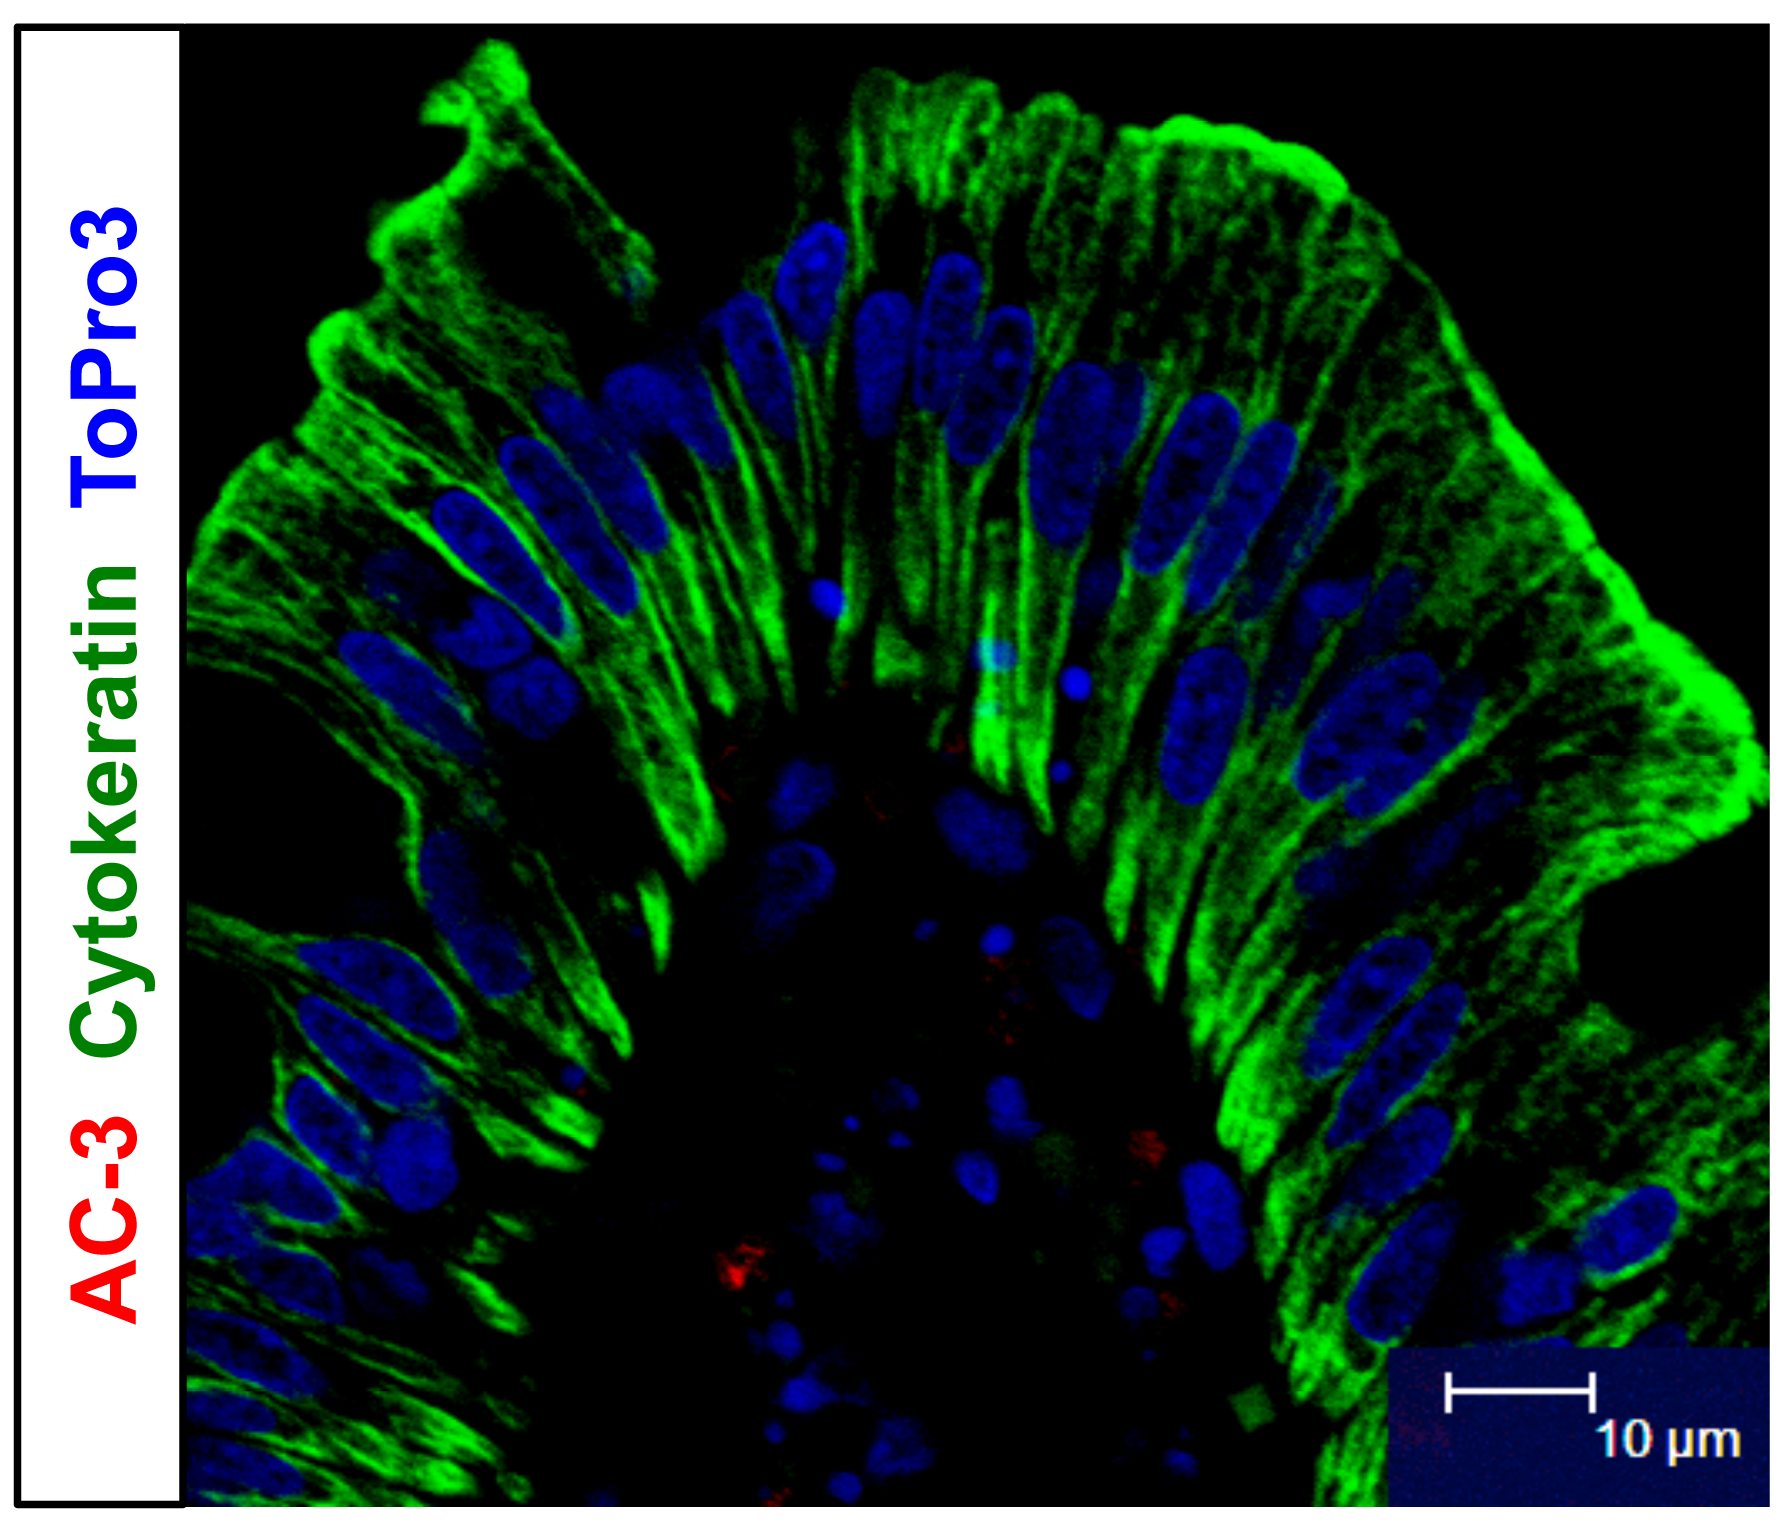
\includegraphics[width=4in]{Epithelial}
\caption{
سلول مخاطی انتهای روده را نشان می‌دهد. اسکلت سلولی با رنگ سبز نشان داده شده است.\cite{10.1371/journal.pone.0030247}
}
\label{fig:Epithelial}
\end{center}
\end{figure}
بافت‌های مخاطی\LTRfootnote{Epithelial}(شکل \ref{fig:Epithelial}) ۶۰ درصد سلول‌های بدن انسان را تشکیل می‌دهند و معمولا بیش از ۹۰ درصد سلول‌های سرطانی از این بافت‌ها شروع می‌شود \cite{doi:10.1080/19336918.2015.1008329}.

تغییر شکل سلول‌های مخاطی و مهاجرت آنها شامل تغییرات در انقباض مکانیکی سلول است که انرژی خود را از اسکلت سلولی اکتومایوسینی تامین می‌کند. فعالیت‌های این سلول از برهمکنش‌ آن با اسکلت خارج سلول و  سلول‌های دیگر تاثیر می‌پذیرد. این سلول‌ها حرکت محدودی دارند و با سرعت کمی مهاجرت می‌کنند. این محدودیت حاصل از اتصالات قوی و قابل انبساط است که شبکه‌ی درونی و بیرونی را تثبیت می‌کند \cite{LANGE20132418}. در رشد تومورِ سلول‌های مخاطی اختلال در فرآیندهای مختلف مثل نقاط اتصال نامنظم و برهمکنش‌های مکانیکی تغییر یافته بین اسکلت درون سلولی و برون سلولی مشاهده شده‌است \cite{LANGE20132418}. در نتیجه رشد بافت تحت تاثیر ساز و کار اتصالات و برهمکنش اسکلت سلولی قرار می‌گیرد. به طور مثال شبکه برون سلولی در تومورهای مخاطی ۵-۲۰ برابر سخت‌تر نسبت به حالت عادی گزارش شده‌است \cite{Paszek:2005qq}. افزایش سختی شبکه برون سلولی ناشی از افزایش نیروهای انقباضی و تعداد نقاط اتصال کانونی است \cite{LANGE20132418}. عکس العمل این نیرو‌ها به سطوحی که سلول روی آن قرار دارد وارد می‌شود و باعث می‌شود که شکل محیط اطراف نیز تغییر کند \cite{PhysRevB.14.3438}.



\subsection{ویسکوالاستیسیته}
مجموعه‌ی اسکلت سلول پاسخ سلول و توزیع نیروی داخل سلول را مشخص می‌کند. در چند بخش  پیشرو سعی شده خصوصیت این شبکه و مدل‌های که رفتار این شبکه ‌را توصیف می‌کنند معرفی شود. برای نوشتن این بخش از منابع \cite{doi, Viscoelasticity, visco} و برای اطلاعات بیشتر توسیه می‌شود که به این منابع مراجعه فرمایید.
\subsubsection{ساز و کار مولکولی}
پلیمرْ\LTRfootnote{Polymer} مولکولی متشکل از رشته‌ی بلندی از اتم‌هاست. عکس العمل یک پلیمر به نیروی خارجی در مقیاس اتمی به دو نوعِ عمومی تقسیم می‌شود. هنگامی که پلیمر تحت تنش قرار می‌گیرد مکان و زاویه اتم‌ها  نسبت به یکدیگر تغییر می‌کند و باعث افزایش انرژی درونی‌ آن می‌شود. مقیاس زمانی این عکس العمل در حدود $\sim10^{-12}$ ثانیه است. در صورت منعطف بود پلیمر  ممکن است که دو اتم آزادی لازم برای چرخیدن نسبت به محور خط واصل‌شان را نیز داشته باشند. مثالا چرخش پلیمر حول پیوند‌ کربن-کربن تغییر زیادی در چیدمان پلیمر‌ها ایجاد می‌کند. همچنین در صورت مناسب بودن ساختار، برخی پلیمر‌ها در راستای تنش کشیده می‌شوند که باعث کاهش انتروپی\LTRfootnote{Entropy}  می‌شود. پلیمر‌های تشکیل دهنده‌ی لاستیک‌ با این فرآیند کار می‌کنند و با تغییرات خیلی کم در پیوند‌های کوالانسی‌شان انرژی درونی‌شان تغییر می‌کند. طبق قانون دوم ترمودینامیک سهم انتروپی در کار انجام شده توسط این فرآیند با دما تعیین می‌شود،
\begin{equation}
fdx=dU-TdS.\label{eq:second_thermo}
\end{equation}
معادله بالا نشان می‌دهد که با تغییر دما می‌توان نقش انتروپی در خواص الاستیکی پلیمر‌ها را مشخص کرد. نتیجه‌ی مستقیم این رابطه همچنین بیان می‌کند که نیروی لازم برای نگه‌داشتن یک نوار الاستیکی در یک طول مشخص به همراه بالا رفتن دما افزایش می‌یابد چرا که انرژی بیشتر صرف غلبه بر حرکات تصادفی پلیمر‌های تشکیل دهنده می‌شود. و در نقطه مقابل در یک میله استیل خواص انتروپی اتم‌ها سهم مهمی در خواص الاستیکی آن ندارند و انبساط دمایی نیروی الاسیتیک میله را کاهش می‌دهد.
البته عوامل فیزیکی و شیمیایی زیادی بر خواص مولکولی پلیمر‌ها تاثیر می‌گذارد، مانند ساختار مولکولی، دما، وجود محلول‌هایی که بر پلیمر اثر ‌می‌گذارند (مثالا محلول‌های که باعث تورم یا متمرکز شدن پلیمر‌ها شوند).  
\subsubsection{گرانروی، الاستیسیته،  و ویسکوالاتستیسیته}
عکس العمل مواد هوکی که تحت تنش مانند شکل \ref{fig:3.2}.الف قرار گرفته‌اند  با رابطه‌ی خطی 
\begin{figure}[htbp]
\begin{center}
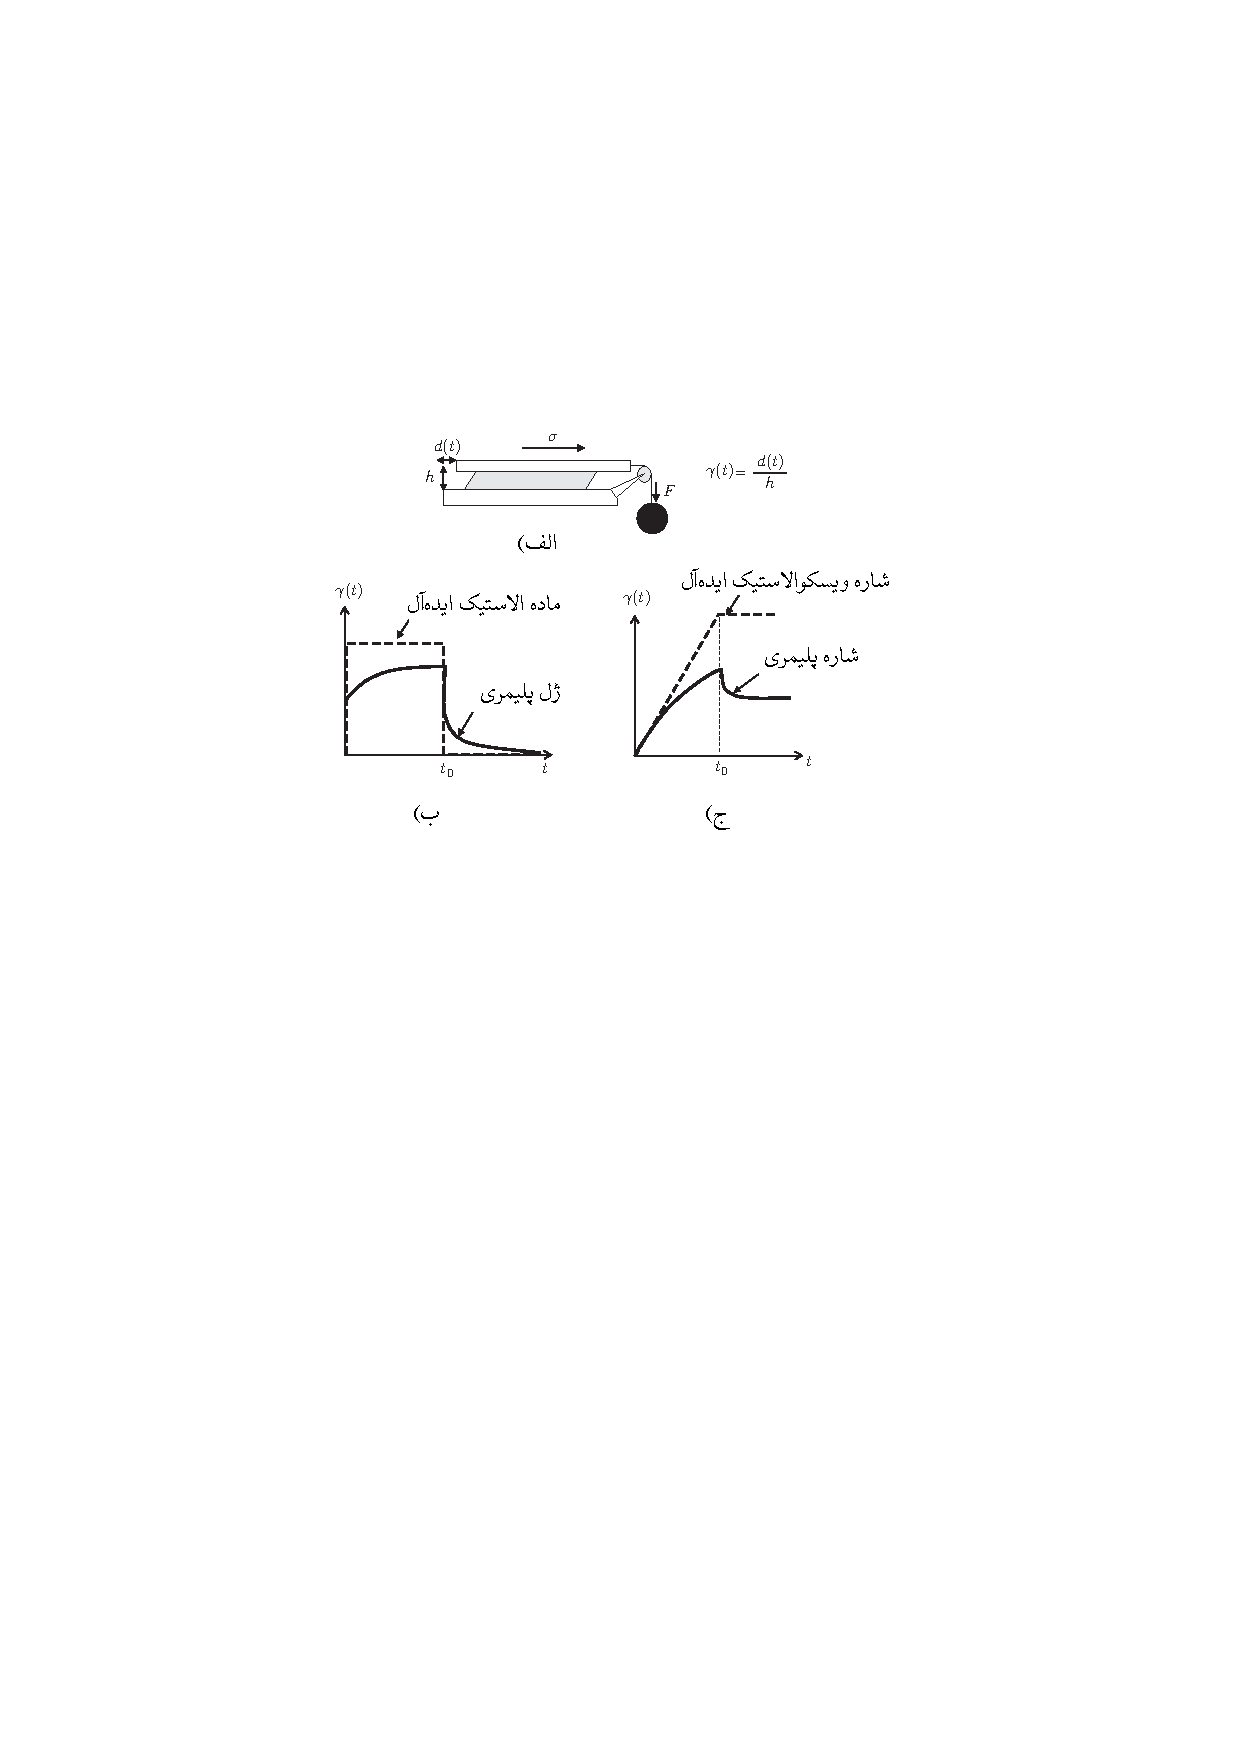
\includegraphics[width=5in]{Fig3_2}
\caption{
الف) یک چیدمان آزمایشگاهی برای اندازه‌گیری خواص مکانیکی مواده را نشان می‌دهد. ماده بین دو صفحه موازی قرار گرفته و در زمان $t=0$  نیروی ثابت $F$ به صفحه بالایی اعمال شده و در زمان $t_0$ نیرو قطع شده‌. ب) پاسخ ماده شبه جامد. ج) پاسخ ماده شبه شاره.
}
\label{fig:3.2}
\end{center}
\end{figure}


\begin{equation}
\sigma=G\gamma
\label{eq:elastic}
\end{equation}
توصیف می‌شود. که در آن $\gamma$ کرنش برشی\LTRfootnote{Shear strain}، $G$ مدول برشی\LTRfootnote{Shear modulus}، و $\sigma$ تنش برشی\LTRfootnote{Shear stress} است. از طرفی عکس العمل شاره نیوتنی تحت تنش مشابه با نرخ تغییر کرنش برشی رابطه‌ی خطی دارد،
\begin{equation}
\sigma=\eta\dot\gamma,
\label{eq:visco}
\end{equation}

که در آن $\eta$ گرانروی شاره است. در مواد نرم معمولا مجموعی از هر دو عکس العمل مشاهده می‌شود که خواصیت ویسکوالاستیکی\LTRfootnote{Viscoelasticity} این مواد را توصیف می‌کند. در شکل \ref{fig:rheo} ساختار ساده‌ای از رئومترها\LTRfootnote{Rheometers} نشان داده شده که بوسیله‌ی آن رفتار ویسکوالستیک مواد مشخص می‌شود. با استفاده از این ابزارها می‌توان تنش یکنواخت و کرنش کنترل شده‌ی وابسته به زمان در ماده ایجاد کرد. البته که می‌توان پاسخ ماده تحت کرنش ثابت و تنش وابسته به زمان را نیز مورد بررسی قرار داد.
\begin{figure}[htbp]
\begin{center}
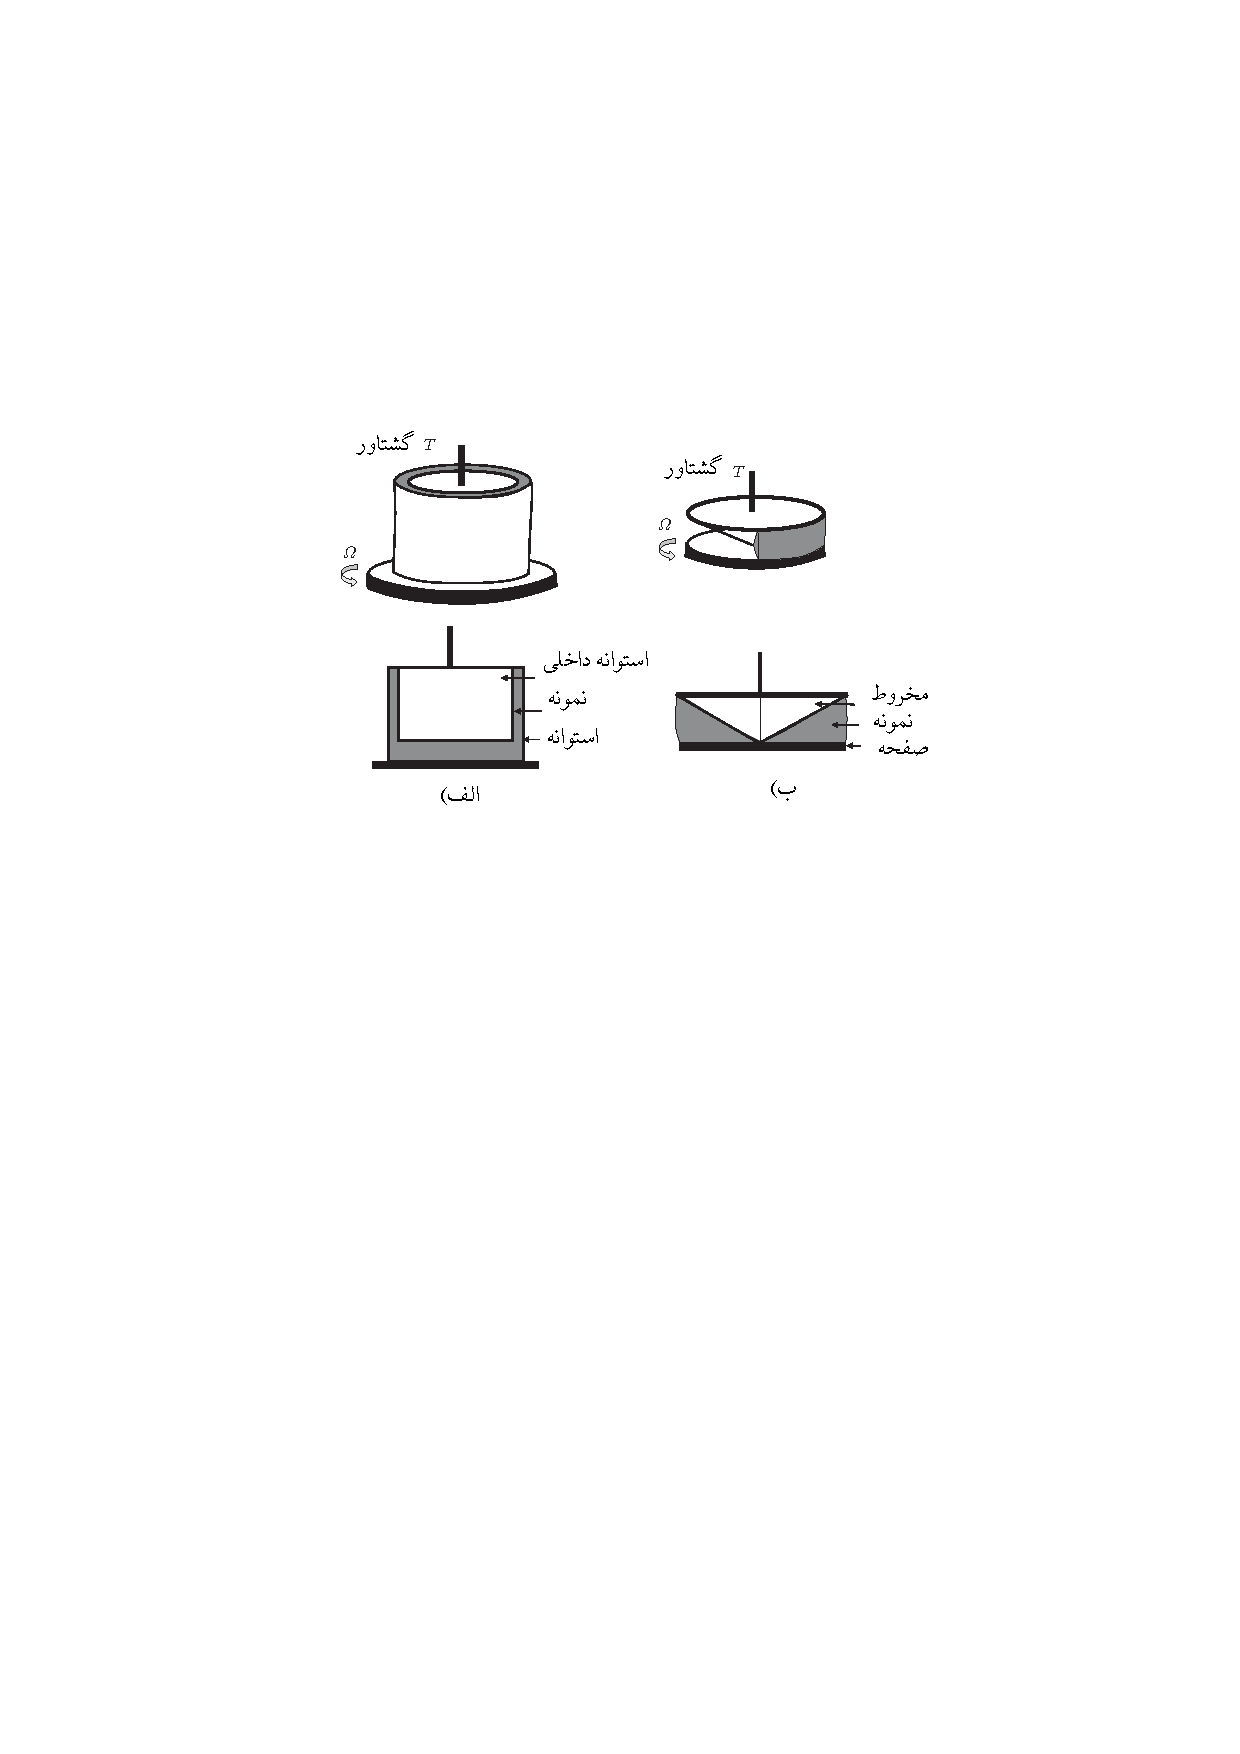
\includegraphics[width=5in]{9_1}
\caption{
ابزارهای مورد استفاده برای اندازه‌گیری خواص ویسکوالاستیکی شاره‌. الف) شاره بین تو استوانه هم محور قرار می‌گیرد. در اینجا با ثبت نگه داشتن استوانه داخلی و چرخاندن استوانه بیرونی کرنش ایجاد می‌شود. اگر فاصله دو استوانه بسیار کم  باشد می‌توان کرنش یکنواخت در ماده ایجاد کرد. نرخ کرنش با اندازهگ‌یری سرعت چرخش و تنش با اندازه‌گیری گشتاور وارد به استوانه داخلی اندازه‌گیری می‌شود. ب) در این ابزار شاره بین یک صفحه و مخروط قرار می‌گیرد. کرنش یکنواخت با چرخاندن صفحه زیرین و ثابت نگه داشتن مخروط ایجاد می‌شود. مشابه ابزار قبل تنش و نرخ کرنش به ترتیب با اندازه‌گیری گشتاور وارد بر مخروط و سرعت چرخیدن صفحه زیرین محاسبه می‌شود.
}
\label{fig:rheo}
\end{center}
\end{figure}
شکل \ref{fig:relax} پاسخ تنش ماده ویسکوالاستیک تحت کرنش پله‌ای (معادله‌ی \ref{eq:step_stress}) را نشان می‌دهد.
\begin{figure}[htbp]
\begin{center}
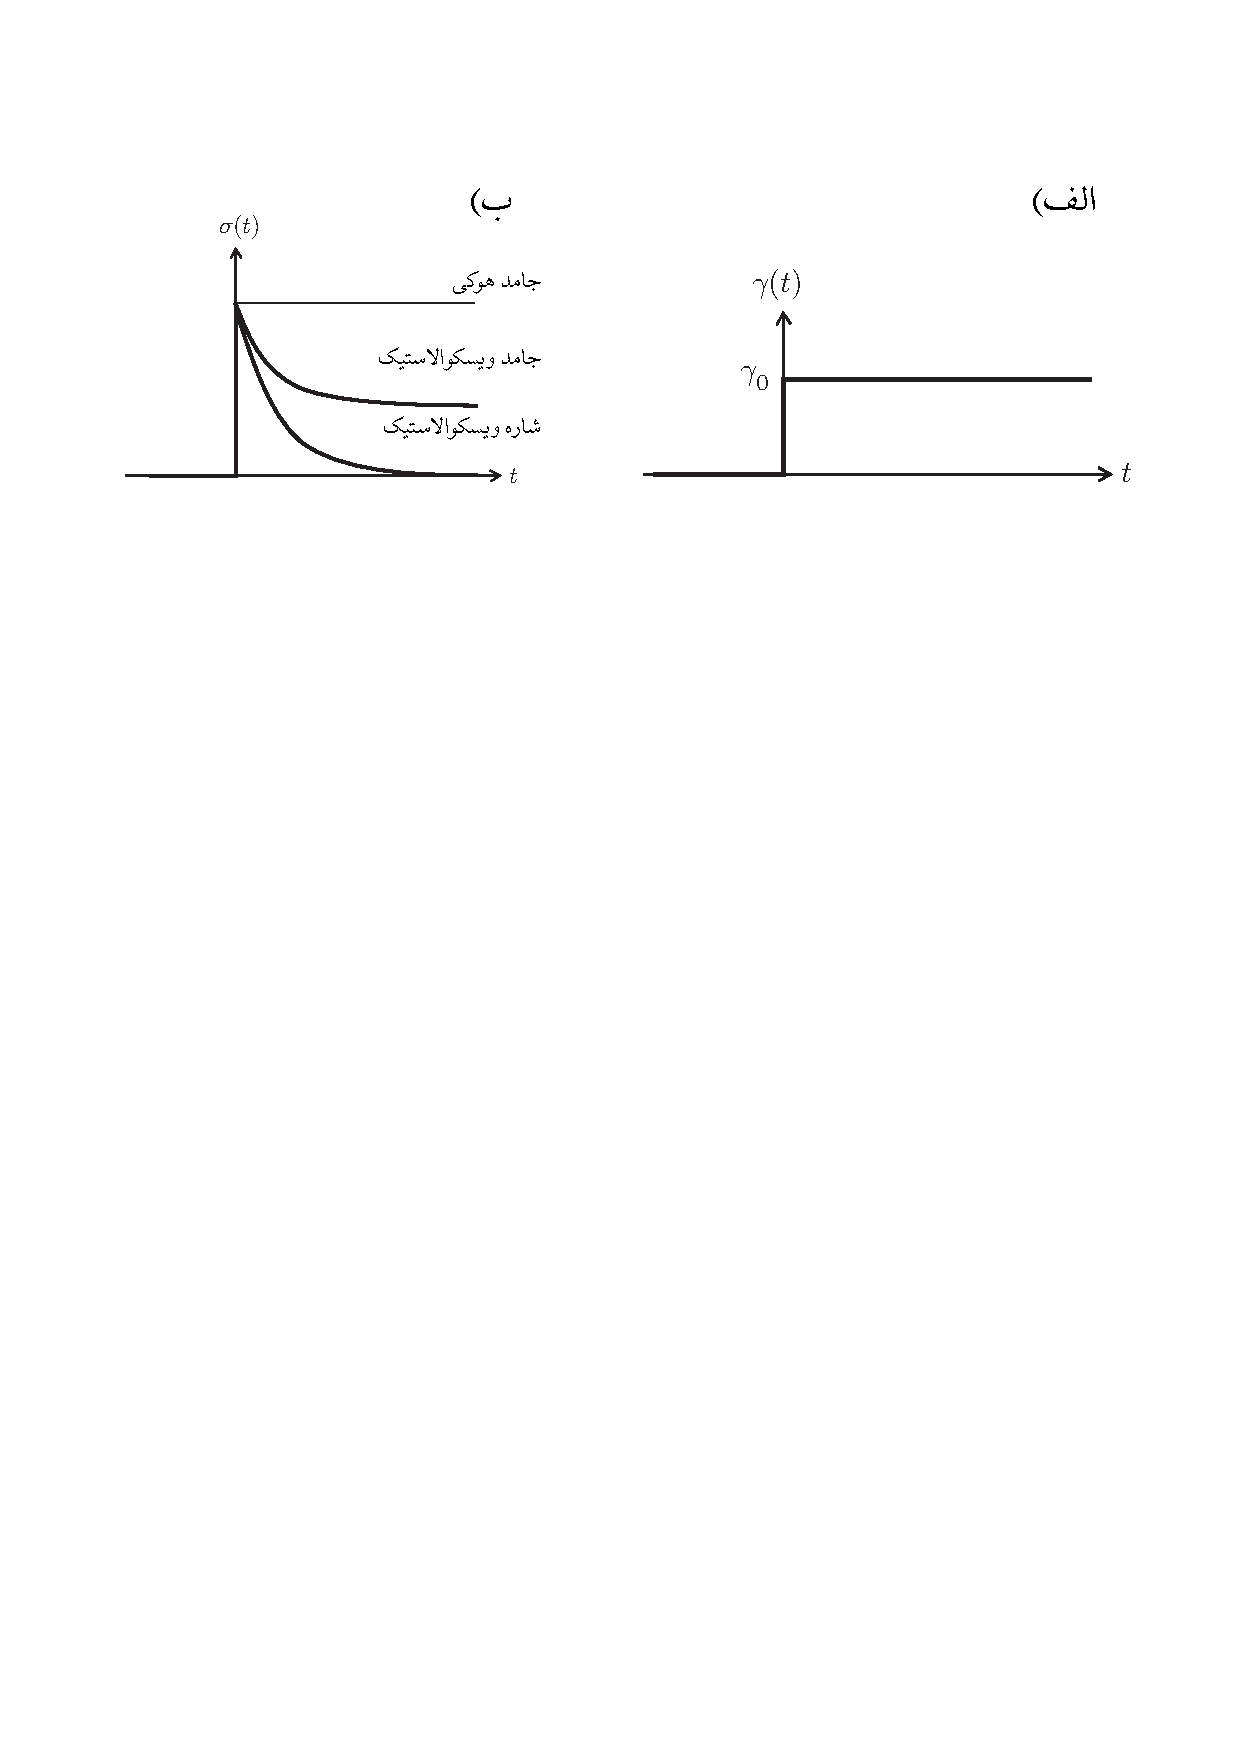
\includegraphics[width=6in]{9_2}
\caption{
آزمایش واحلش تنش را نشان می‌دهد. کرنش پله‌ای که در شکل الف) نشان داده شده به ماده اعمال شده و تنش ایجاد شده اندازه‌گیری می‌شود. و در شکل ب) پاسخ مواد مختلف نشان داده ‌شده‌است.
}
\label{fig:relax}
\end{center}
\end{figure}

\begin{equation}
\begin{aligned}
%\{ 
\gamma(t)=\gamma_0\Theta(t)=
  \begin{cases}
    0       & t<0\\
    \gamma_0  & t>0
  \end{cases}
%\}
\end{aligned}\label{eq:step_stress}
\end{equation}
عکس العمل ماده تابع $\gamma_0$ کرنش اولیه، و زمان خواهد بود. برای کرنش‌های کوچک می‌توان تنش را به این صورت نوشت،
\begin{equation}
\sigma(t)=\gamma_0G(t).
\end{equation}
تابع $G(t)$ مدول واحلش\LTRfootnote{Relaxationn modulus} است. شکل \ref{fig:relax} مدول واحلش مواد مختلف را به صورت کیفی رسم می‌کند. همانطور که پیش‌تر اشاره شد رابطه‌ی کرنش و تنش برای جامد الاستیکی (هوکی، نیوتنی) خطی است و تحت کرنش ثابت تنش ثابت در ماده ایجاد می‌شود. مذاب پلیمری و محلول‌های پلیمری تحت کرنش ثابت ابتدا مقوامت می‌کنند و در ماده تنش ایجاد می‌شود. از آنجایی که محلول پلیمری مقید به حفظ شکل مشخصی نیست، با گذشت زمان و جابجایی پلیمر‌های محلول تنش به صفر کاهش پیدا می‌کند. این مواد را شاره‌های ویسکوالاستیک می‌نامیم. در جامد ویسکوالاستیک همچون لاستیک، همانطور که در بخش قبل صحبت شد، پلیمرها شکل‌ خود را حفظ می‌کنند ولی تحت تنش خارجی با تغییر شکل محدود می‌توانند انرژی درونی خود را افزایش دهند. در نتیجه پس از اعمال کرنش تنش با جابجایی و تغییر شکل پلیمر‌ها کاهش می‌یابد ولی صفر نمی‌شود.
\subsubsection{گرانروی خطی}

تنش مواد ویسکوالاستیک به کرنشی که در زمان‌های گذشته اعمال شده بستگی دارد. در نتیجه رفتار مواد ویسکوالاستیک بسیار پیچیده است. در صورتی که کرنش کوچک باشد به طوری که سیستم از حالت تعادلی خیلی دور نباشد اصل برهمنهی پابرجا خواهد بود\cite{doi}. در این صورت اگر در زمان $t_1$ کرنش $\gamma_(t_1)$ به سیستم اعمال شود پ تنش $\sigma(t_1)$ و در  زمان $t_2$ کرنش $\gamma_(t_2)$ به سیستم اعمال شود پ تنش $\sigma(t_2)$ ایجاد شود بر اساس اصل برهمنهی کرنش و تنش سیستم،
\begin{equation}
\begin{aligned}
\sigma=\sigma(t_1)+\sigma(t_2) \\
\gamma=\gamma(t_1)+\gamma(t_2)
\end{aligned}
\end{equation}
خواهد بود. اگر تغییرات کرنش بسیار کوچک باشد می‌توان به کمک اصل برهمنهی نوشت،
\begin{equation}
\Delta\gamma_i=\dot\gamma+\Delta t_i
\end{equation}
در نتیجه اگر کرنش پیچیده‌ای به سیستم اعمال شود، می‌توان فرض کرد کرنش کلی مجموعه‌ای از کرنش‌هایی است که در بازه‌های زمانی کوچکی به سیستم وارد می‌شود(شکل \ref{fig:super}) و که قابل توجیه با یک مدول واحلش است، 

\begin{equation}
\gamma(t)=\sum_i\Delta\gamma_i\Theta(t-t_1)
\end{equation}
در نتیجه هر کرنش مقطعی، $\Delta\gamma_i$ در زمان $t_i$ در سیستم تنش $G(t-t_i)\Delta\gamma_i$ را در زمان $t$ ایجاد می‌کند. پس تنش در هر زمان را می‌توان بر اساس مجموع کرنش‌هایی که در گذشته به سیستم وارد شده توصیف کرد،

\begin{equation}
\sigma(t)=\sum_iG(t-t_i)\Delta\gamma_i=\sum_iG(t-t_i)\dot\gamma(t_i)\Delta t.
\end{equation}
و اگر حد بازه‌های زمانی بسیر کوچک را در نظر بگیریم،‌ $\Delta t\rightarrow0$، 
\begin{equation}
\sigma(t)=\int_{-\infty}^tdt'G(t-t')\dot\gamma(t').
\label{eq:sigma}
\end{equation}
رفتار هر ماده‌ای که با اصل برهمنهی با استفاده معادله فوق قابل توصیف باشد را ماده ویسکوالاستیک خطی می‌نامیم. از آنجایی که یک مدول واحلش رفتار سیستم را توصیف می‌کند با داشتن مدول برای یک سیستم می‌توانیم پاسخ تنش سیستم را نسبت به هر کرنشی محاسبه کنیم. به طور مثال، اگر در زمان صفر به سیستم کرنش با نرخ ثابت وارد شود، 
\begin{equation}
\sigma(t)=\int_{-\infty}^tdt'G(t-t')\dot\gamma(t')=\dot\gamma\int_{-\infty}^tdt'G(t-t')
\end{equation}
در صورتی که که در زمان بسیار طولانی این جمع مقدار محدودی شود، با توجه به معادله \ref{eq:visco}،

\begin{equation}
\eta_0=\int_{-\infty}^tdt'G(t-t').
\end{equation}
که تعریف گرانروی در مواد ویسکوالاستیک خطی‌ است.


\begin{figure}[htbp]
\begin{center}
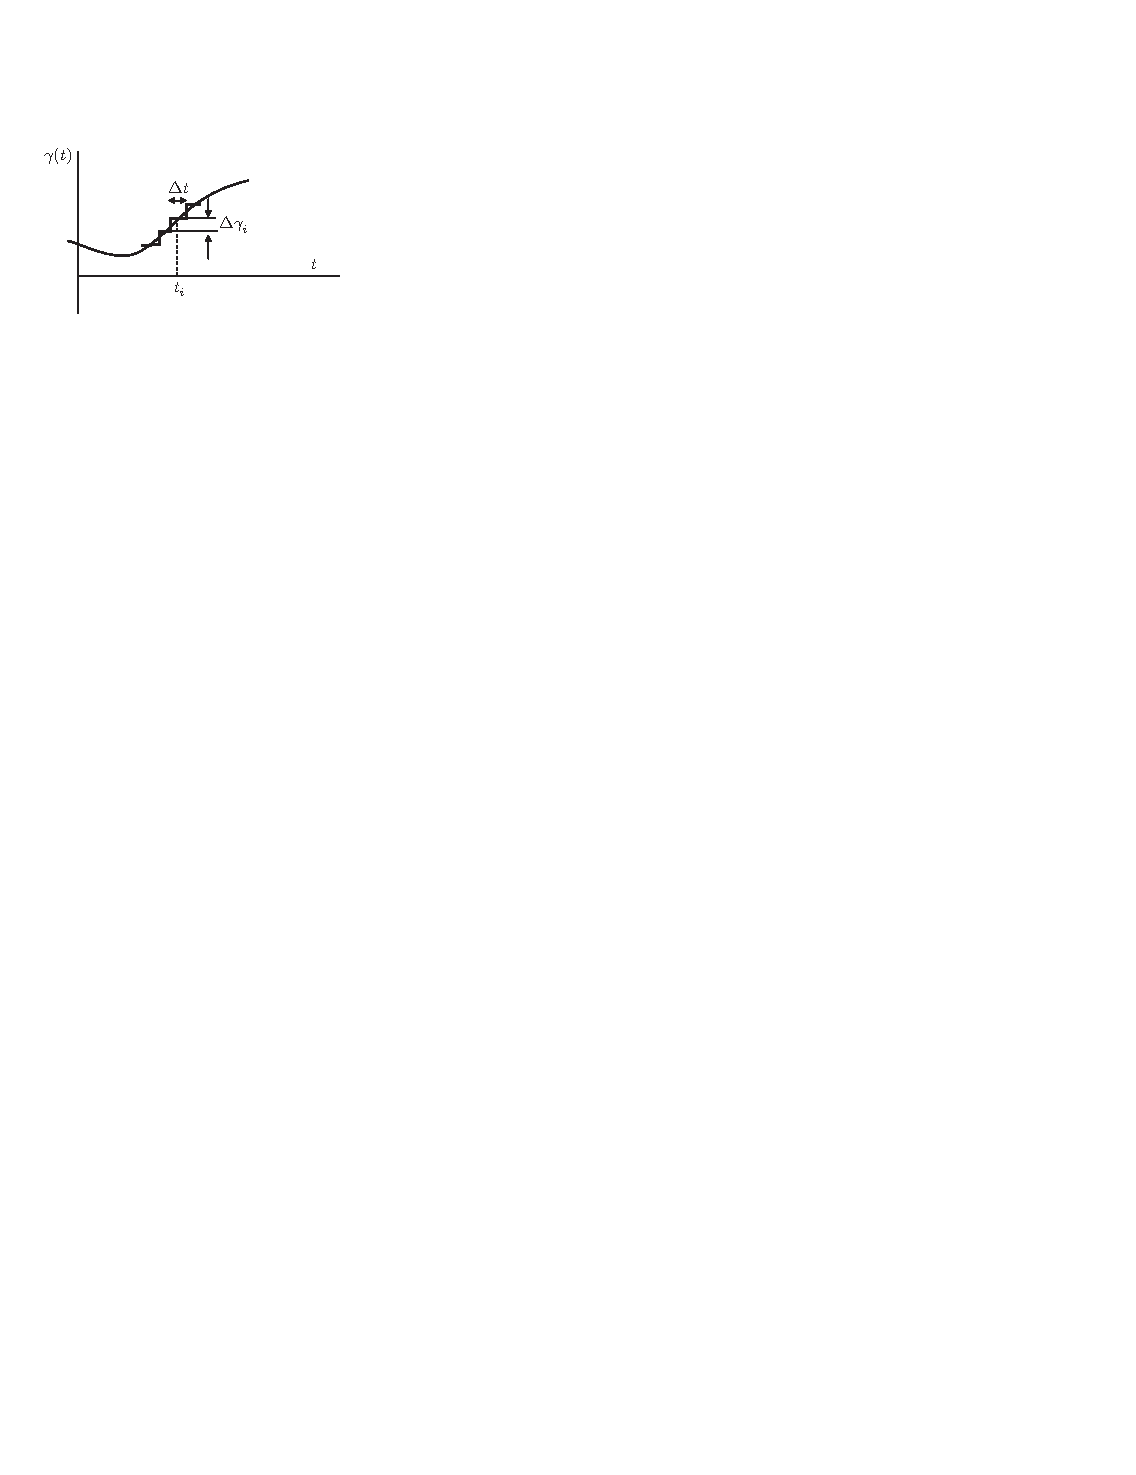
\includegraphics[width=4in]{9_3}
\caption{
با توجه به اصل برهمنهی می‌توان هر کرنش وابسته به زمان را به صورت جمعی از کرنش‌های پله‌ای با اندازه $\Delta\gamma_i$  نشان داد که در زمان $t_i$ به ماده اعمال شده‌است.
}
\label{fig:super}
\end{center}
\end{figure}


\subsubsection{مدل‌سازی رفتار ویسکوالاستیک}

معادله‌ی \ref{eq:elastic} با یک فنر معمولی و معادله‌ی \ref{eq:visco} با دش پات\LTRfootnote{Dash pot} مدل می‌شود و رفتار کرنش برشی این دو مدل هنگامی که تنش برشی خارجی اعمال می‌شود به ترتیب در شکل \ref{fig:3.2} ب و ج با خط چین مشخص شده‌است.
\subsubsection{مدل ماکسول}
مدل ماکسول یک فنر و یک دش پات است که ماههد شکل \ref{fig:SD} به صورت سری به هم متصل شده‌است.

\begin{figure}[htbp]
\begin{center}
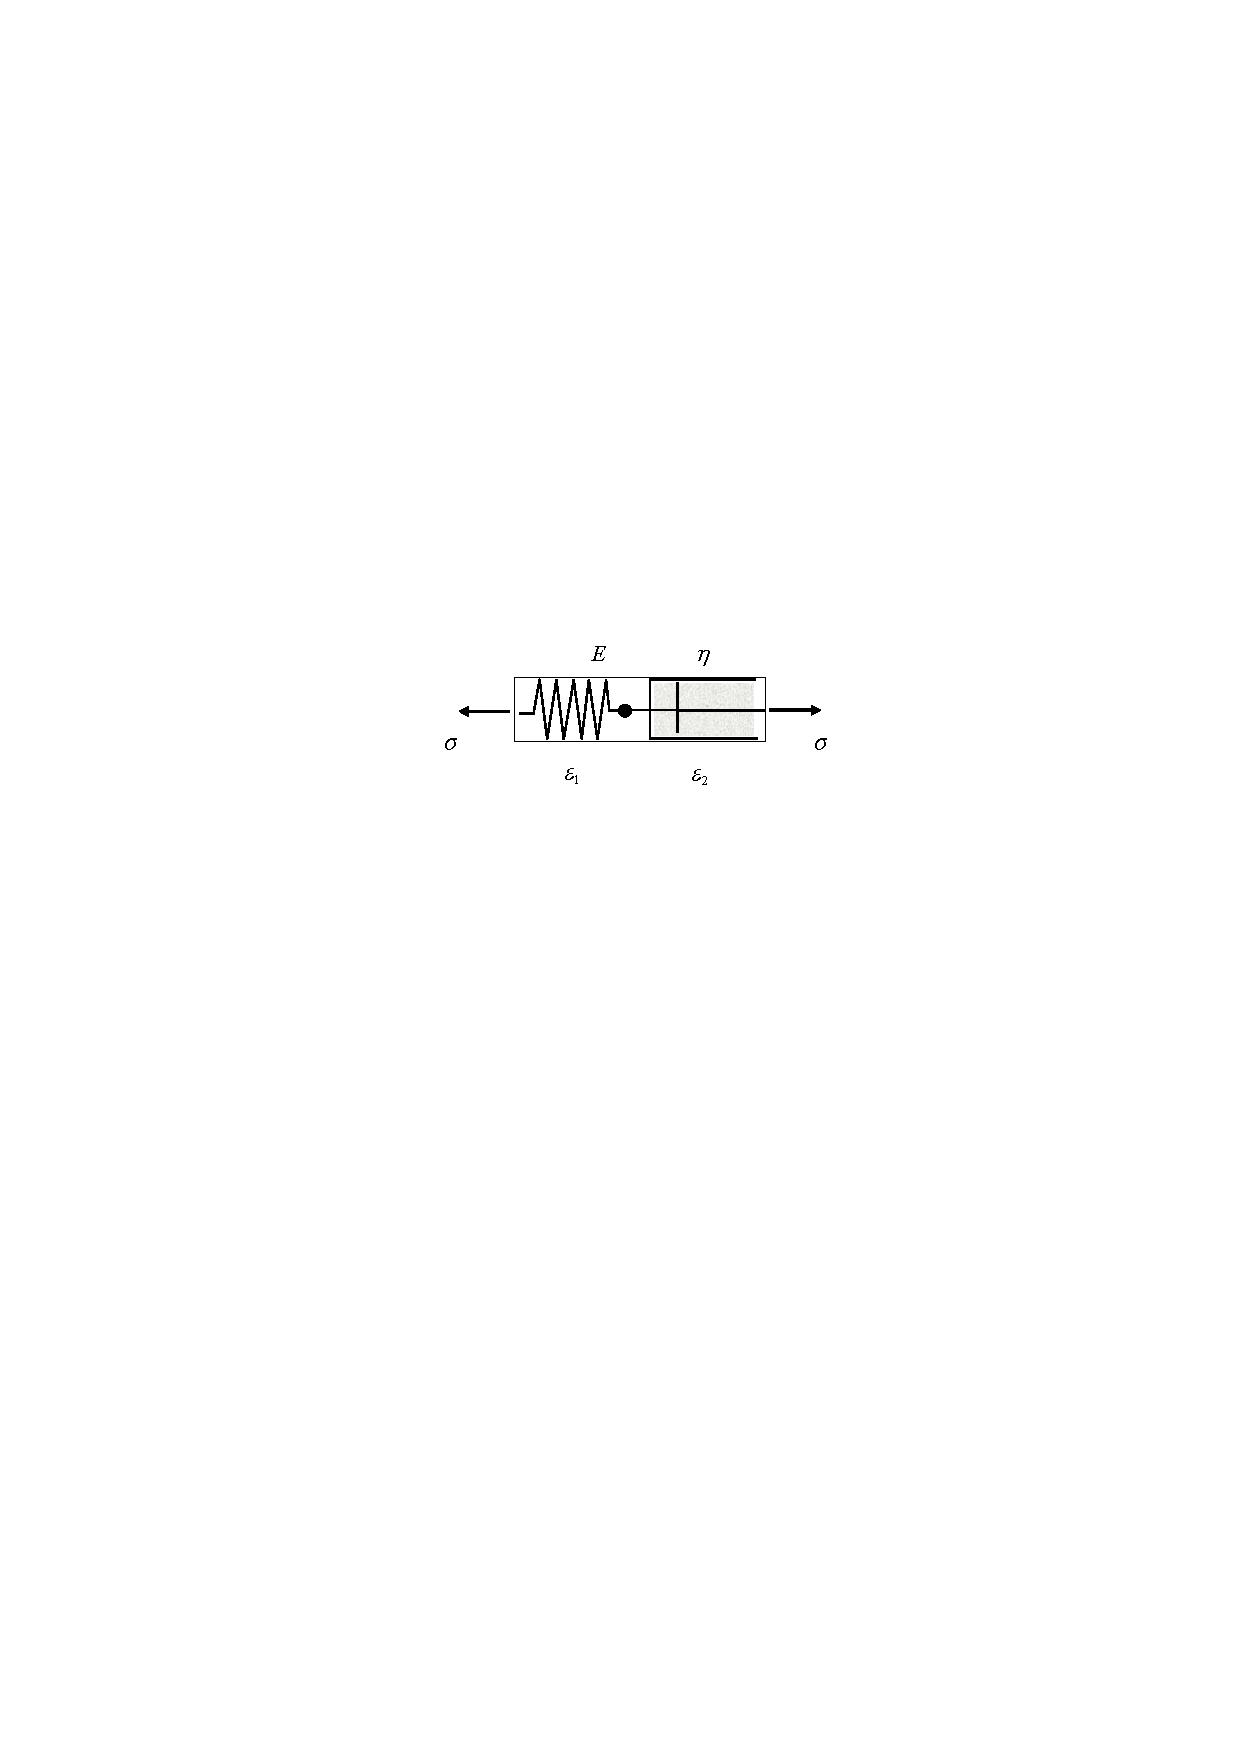
\includegraphics[width=4in]{spring_dashpot}
\caption{
مدل ماکسول
}
\label{fig:SD}
\end{center}
\end{figure}

حالت تعادلی این سیستم زمانیس است که تنش برشی دو قسمت با هم برابر باشد. پس،
\begin{equation}
\gamma_1=\frac{\sigma}{G}, \quad \dot\gamma_2=\frac{\sigma}{\eta}, \quad \gamma=\gamma_1+\gamma_2.
\end{equation}
با مشتق‌گیری و جایگذاری به معادله‌ی زیر می‌رسیم که معادله‌ی ماکسول است،
\begin{equation}
\sigma+\frac{\eta}{G}\dot\sigma=\eta\dot\gamma.
\label{eq:maxwell}
\end{equation}
اگر در زمان صفر تنش برشی $\sigma_0$ به سیستم وارد شود، فنر به سرعت عکس العمل نشان می‌دهد ولی دش پات نیاز به زمان بیشتری دارد که عکس العمل نشان دهد. پس در زمان صفر
\begin{equation}
\gamma_0=\frac{\sigma_0}{G}
\end{equation}
حال کافی‌ است از  معادله‌ی \ref{eq:maxwell}  انتگرال بگریم و شرایط اولیه را جایگذاری کنیم،

\begin{equation}
\dot\gamma=\frac{\sigma_0}{\eta}\rightarrow \gamma(t)=\frac{\sigma_0}{\eta}t+\gamma_0\rightarrow \gamma(t)=\sigma_0\left(\frac{1}{\eta}t+\frac{1}{G}\right).
\end{equation}
حال اگر تنش برشی خارجی را برداریم دوباره شاهد عکس العمل بلافاصله فنر خواهیم بود ولی دش پات علاقه‌ای به از دست دادن کرنش برشی ندارد. این رفتار در شکل \ref{fig:creep_maxwell} نشان داده شده‌است.

\begin{figure}[htbp]
\begin{center}
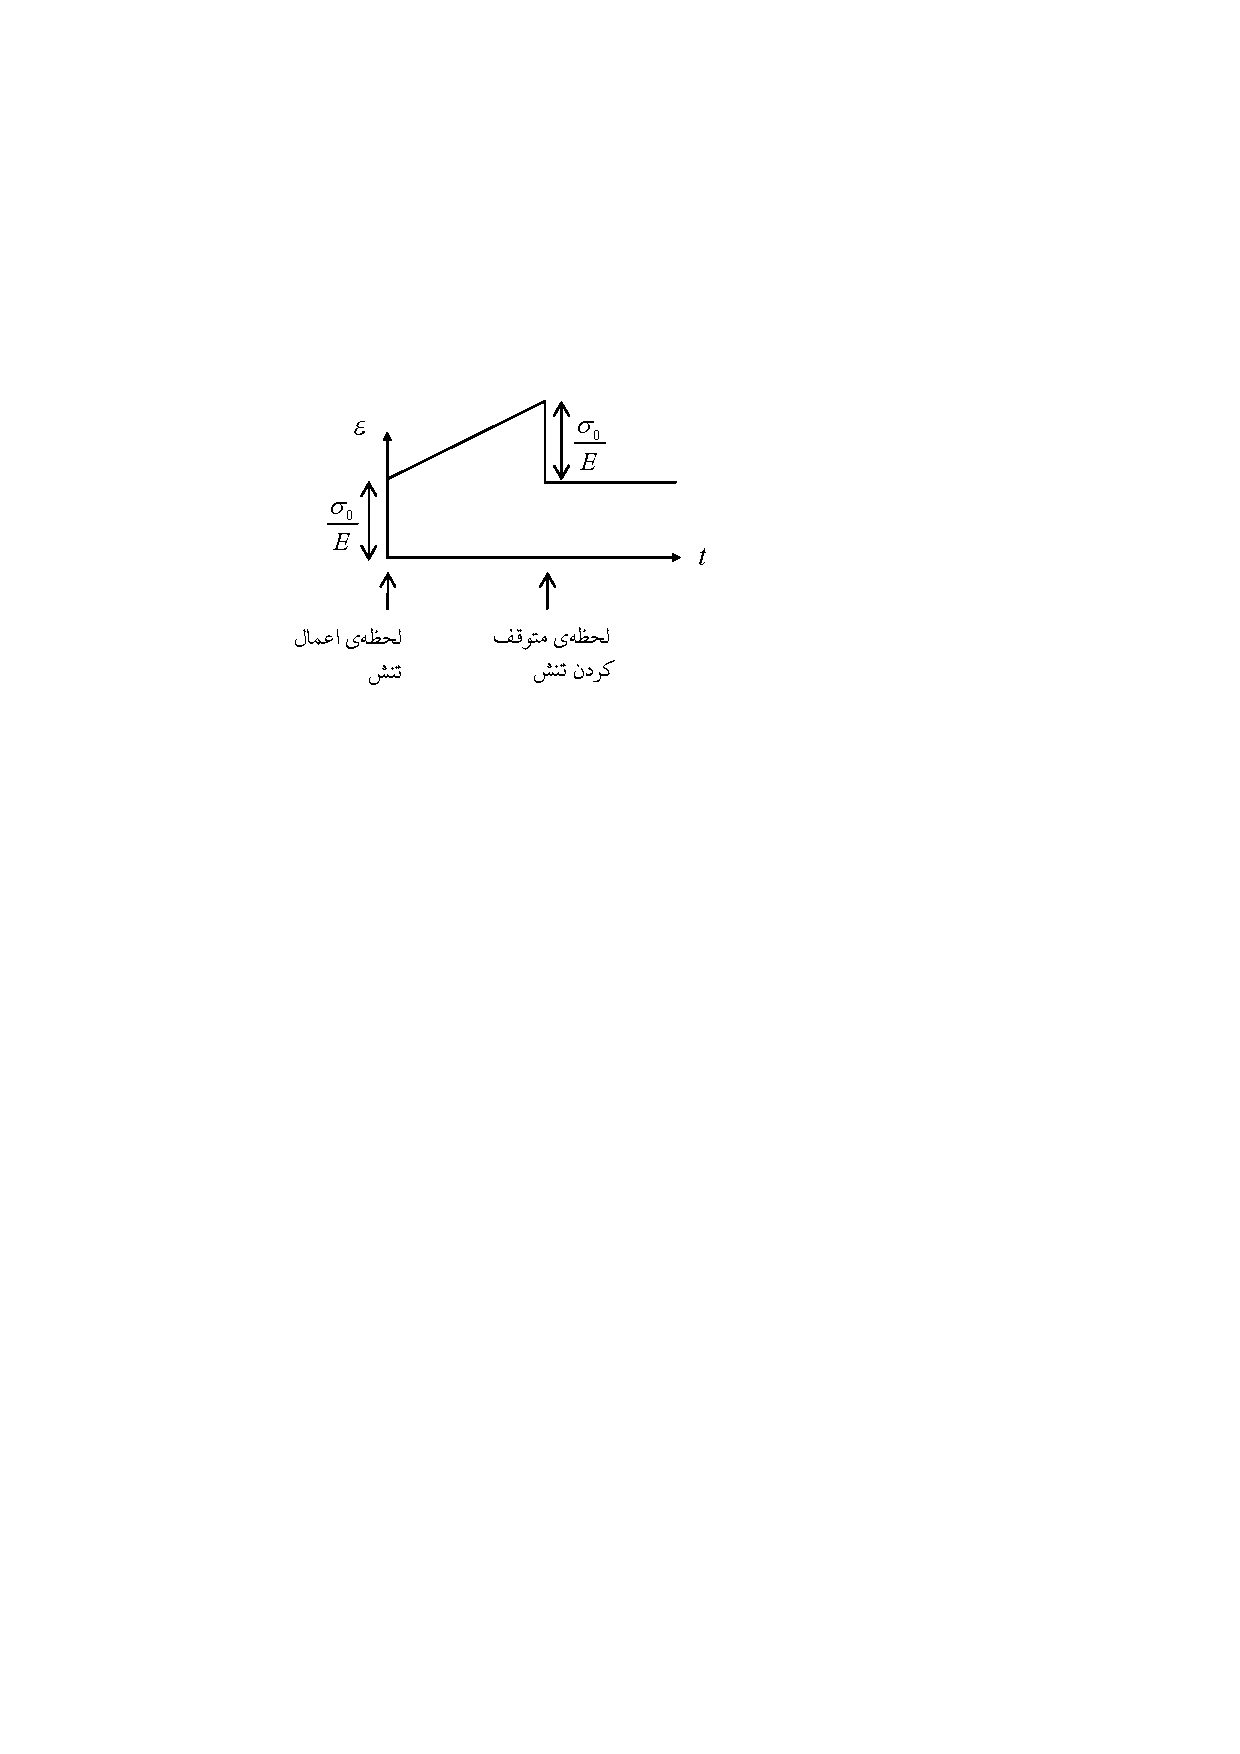
\includegraphics[width=3in]{creep_maxwell}
\caption{
رفتار کردنش در مدل ماکسول هنگامی که در زمان صفر تنش برشی وارد شود و در زمانی بعد این تنش برداشته شود.
}
\label{fig:creep_maxwell}
\end{center}
\end{figure}

\subsubsection{مدل کلوین (وُیت)}
در مدل کلوین\LTRfootnote{Kelvin} یا وُیت\LTRfootnote{Voigt} دو عنصر فنر و دش پات را به صورت موازی به هم متصل می‌کنیم (شکل \ref{fig:KV})
\begin{figure}[htbp]
\begin{center}
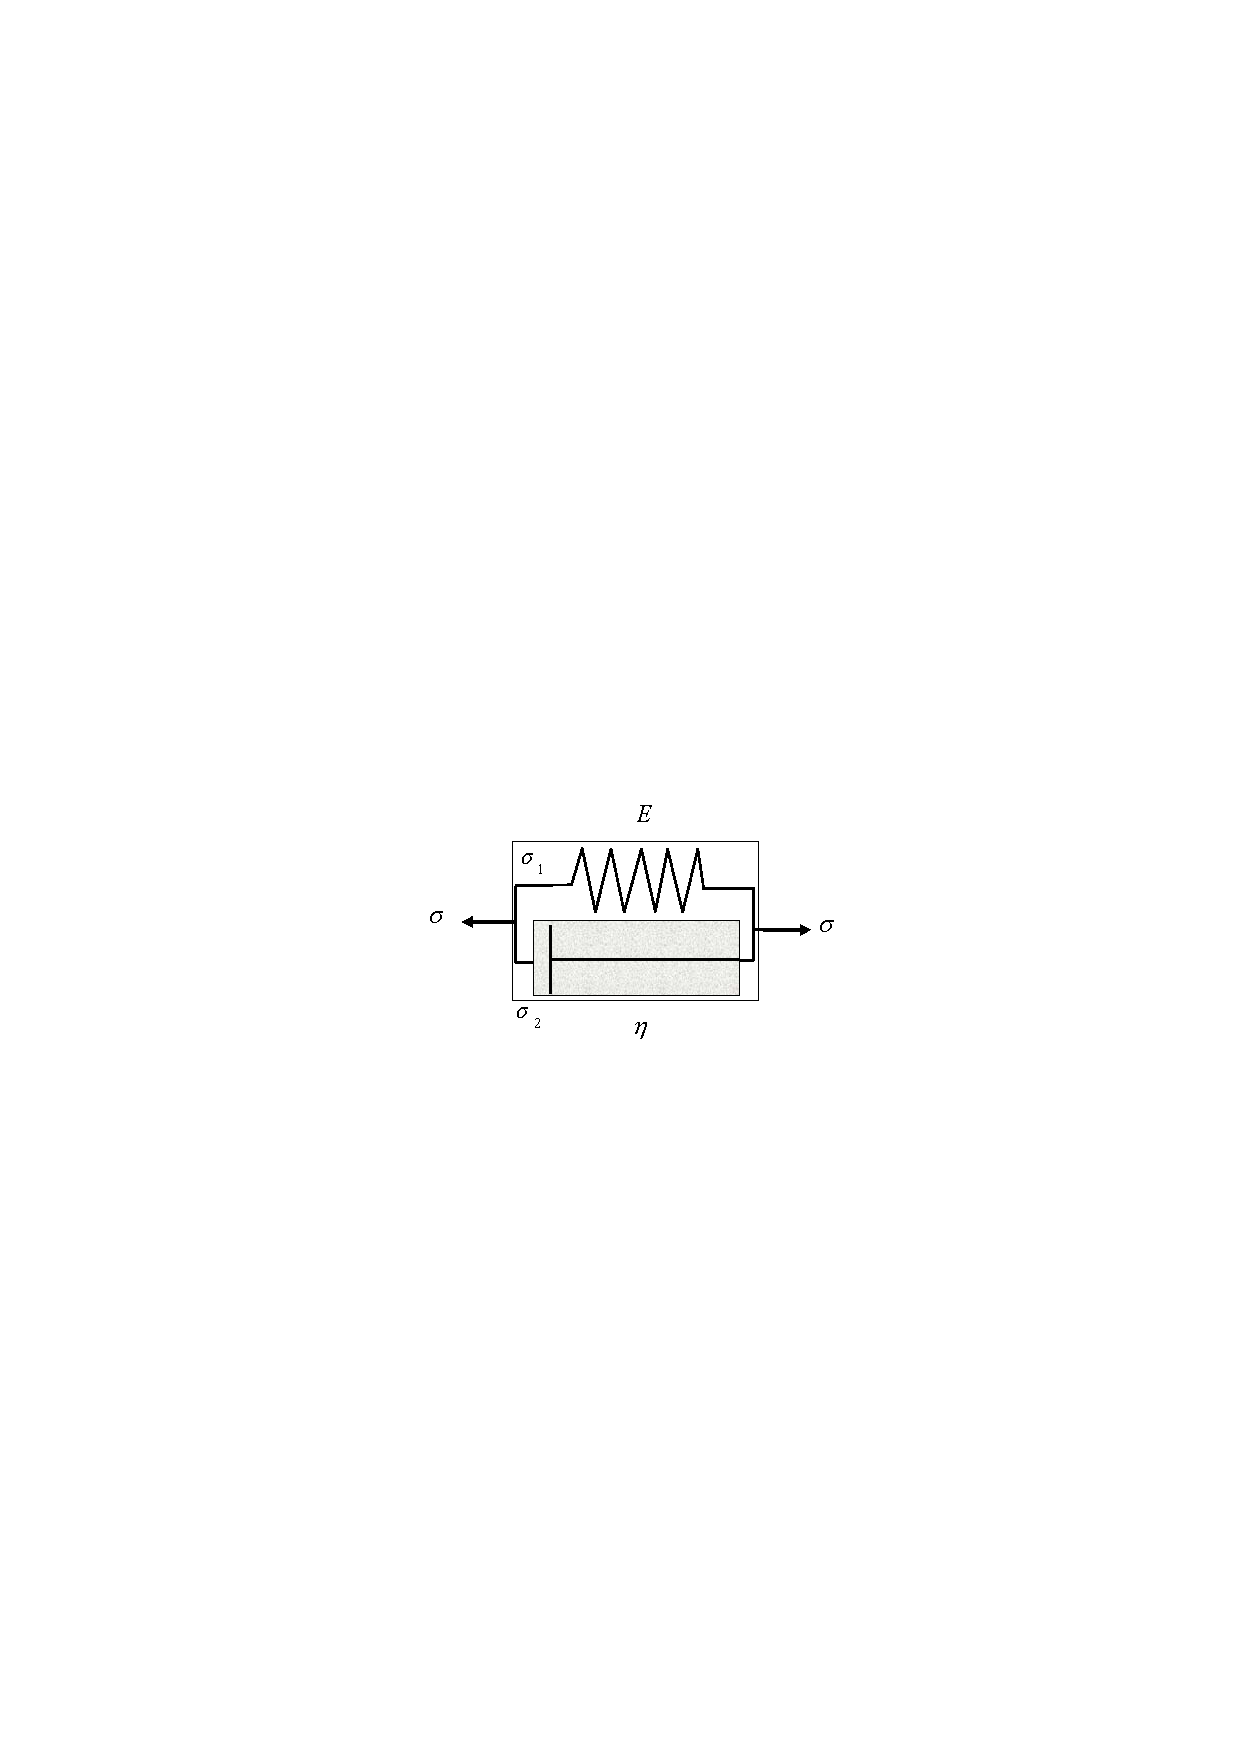
\includegraphics[width=4in]{kelvin_voigt}
\caption{
مدل کلوین یا وُیت را نشان می‌دهد.
}
\label{fig:KV}
\end{center}
\end{figure}
در حالت تعادلی این مدل خمش وجود ندارد در نتیجه کرنش برشی برای هر دو عنصر باید برابر باشد،
\begin{equation}
\gamma=\frac{\sigma_1}{G}, \quad \dot\gamma=\frac{\sigma_2}{\eta}, \quad \sigma=\sigma_1+\sigma_2.
\end{equation}
با یک جایگذاری ساده به معادله کلوین (وُیت) می‌رسیم،
\begin{equation}
\sigma=G\gamma+\eta\dot\gamma
\label{eq:KV}
\end{equation}
اگر در زمان صفر به این سیستم تنش برشی اعمال کنیم، فنر علاقه به افزایش طور دارد ولی دش پات نمی‌تواند تغییر طول دهد، پس تمام تنش به دش پات منتقل می‌شود و کرنش اولیه سیستم صفر است ولی با شیب اولیه‌ی $\sigma_0/\eta$ شروع می‌شود. با گذشت زمان دش پات تغییر طور می‌دهد و قسمتی و در سیستم کرنش برشی ایجاد می‌شود. در طول زمان با تغییر طول از  تنش برشی دش پات کاسته می‌شود و به تنش برشی فنر اضافه می‌شود. با گذشت زمان بسیار طولانی تنش دش پات صفر می‌شود تمام تنش را فنر تحمل می‌کند ($\sigma_0/G$).
معادله درجه اول غیر همگن \ref{eq:KV} را با شرایط اولیه توصیف شده حل می‌کنیم،
\begin{equation}
\gamma(t)=\frac{\sigma_0}{G}\left(1-e^{-\frac{t}{t_R}}\right), \quad t_R=\frac{\eta}{G}.
\end{equation}
زمان مشخصه $t_R$ زمان بازماندگی\LTRfootnote{Retardation time} سیستم است. حال اگر در زمان $\tau$ تنش را از سیستم برداریم دوباره فنر علاقه به تغییر طول دارد ولی دش پات اجازه نمی‌دهد و تمام تنش سیستم را تحمل می‌کند. حل معادله‌ی \ref{eq:KV} با کرنش صفر به شکل زیر خواهد بود،
\begin{equation}
0=G\gamma+\eta\dot\gamma \rightarrow Ce^{-\frac{t}{t_R}}.
\end{equation}
با محاسبه‌ی تنش در زمان $t=\tau$ و جایگذاری در معادله‌ی بالا،
\begin{equation}
\gamma(t)=\frac{\sigma_0}{G}e^{-\frac{t}{t_R}}\left(e^{\frac{\tau}{t_R}}-1\right), \quad t>\tau
\end{equation}
رفتار معادله‌ی فوق در شکل \ref{fig:creep_KV} نمایش داده شده‌است.
\begin{figure}[htbp]
\begin{center}
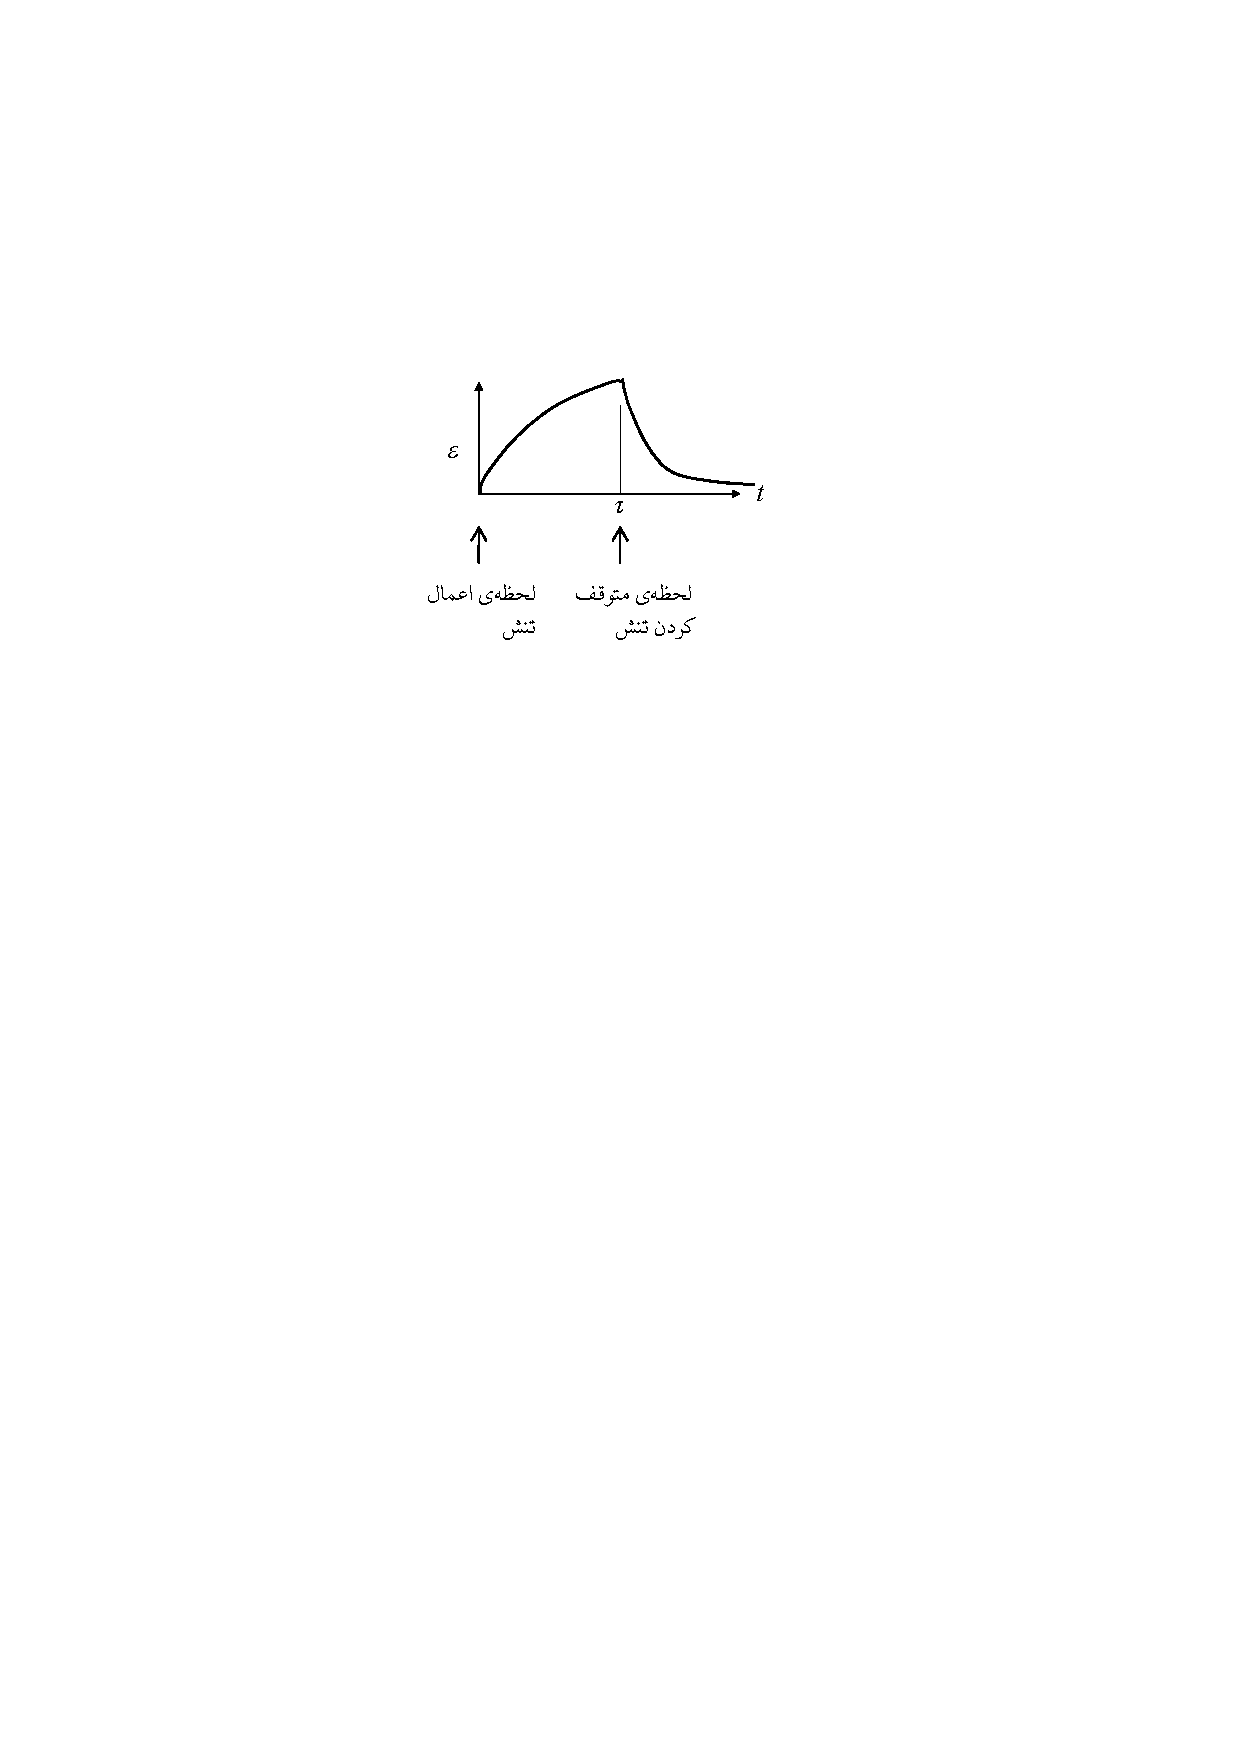
\includegraphics[width=3in]{creep_KV}
\caption{
رفتار کرنش برشی برای مدل کلوین (وُیت) را نشان می‌دهد. در زمان صفر تنش $\sigma_0$ به سیستم وارد می‌شده و در زمان $t=\tau$ بار از روی سیستم برداشته می‌شود.
}
\label{fig:creep_KV}
\end{center}
\end{figure}
\subsubsection{مدل‌های ۳ عنصری}
ترکیب دو مدل ماکسول و کلوین ساده‌ترین مدلی است که می‌تواند رفتار عمومی مواد ویسکوالستیک را توصیف کند. ۴ ترکیب ممکن مدل ۳ عنصری در شکل \ref{fig:MK} رسم شده‌است.
\begin{figure}[htbp]
\begin{center}
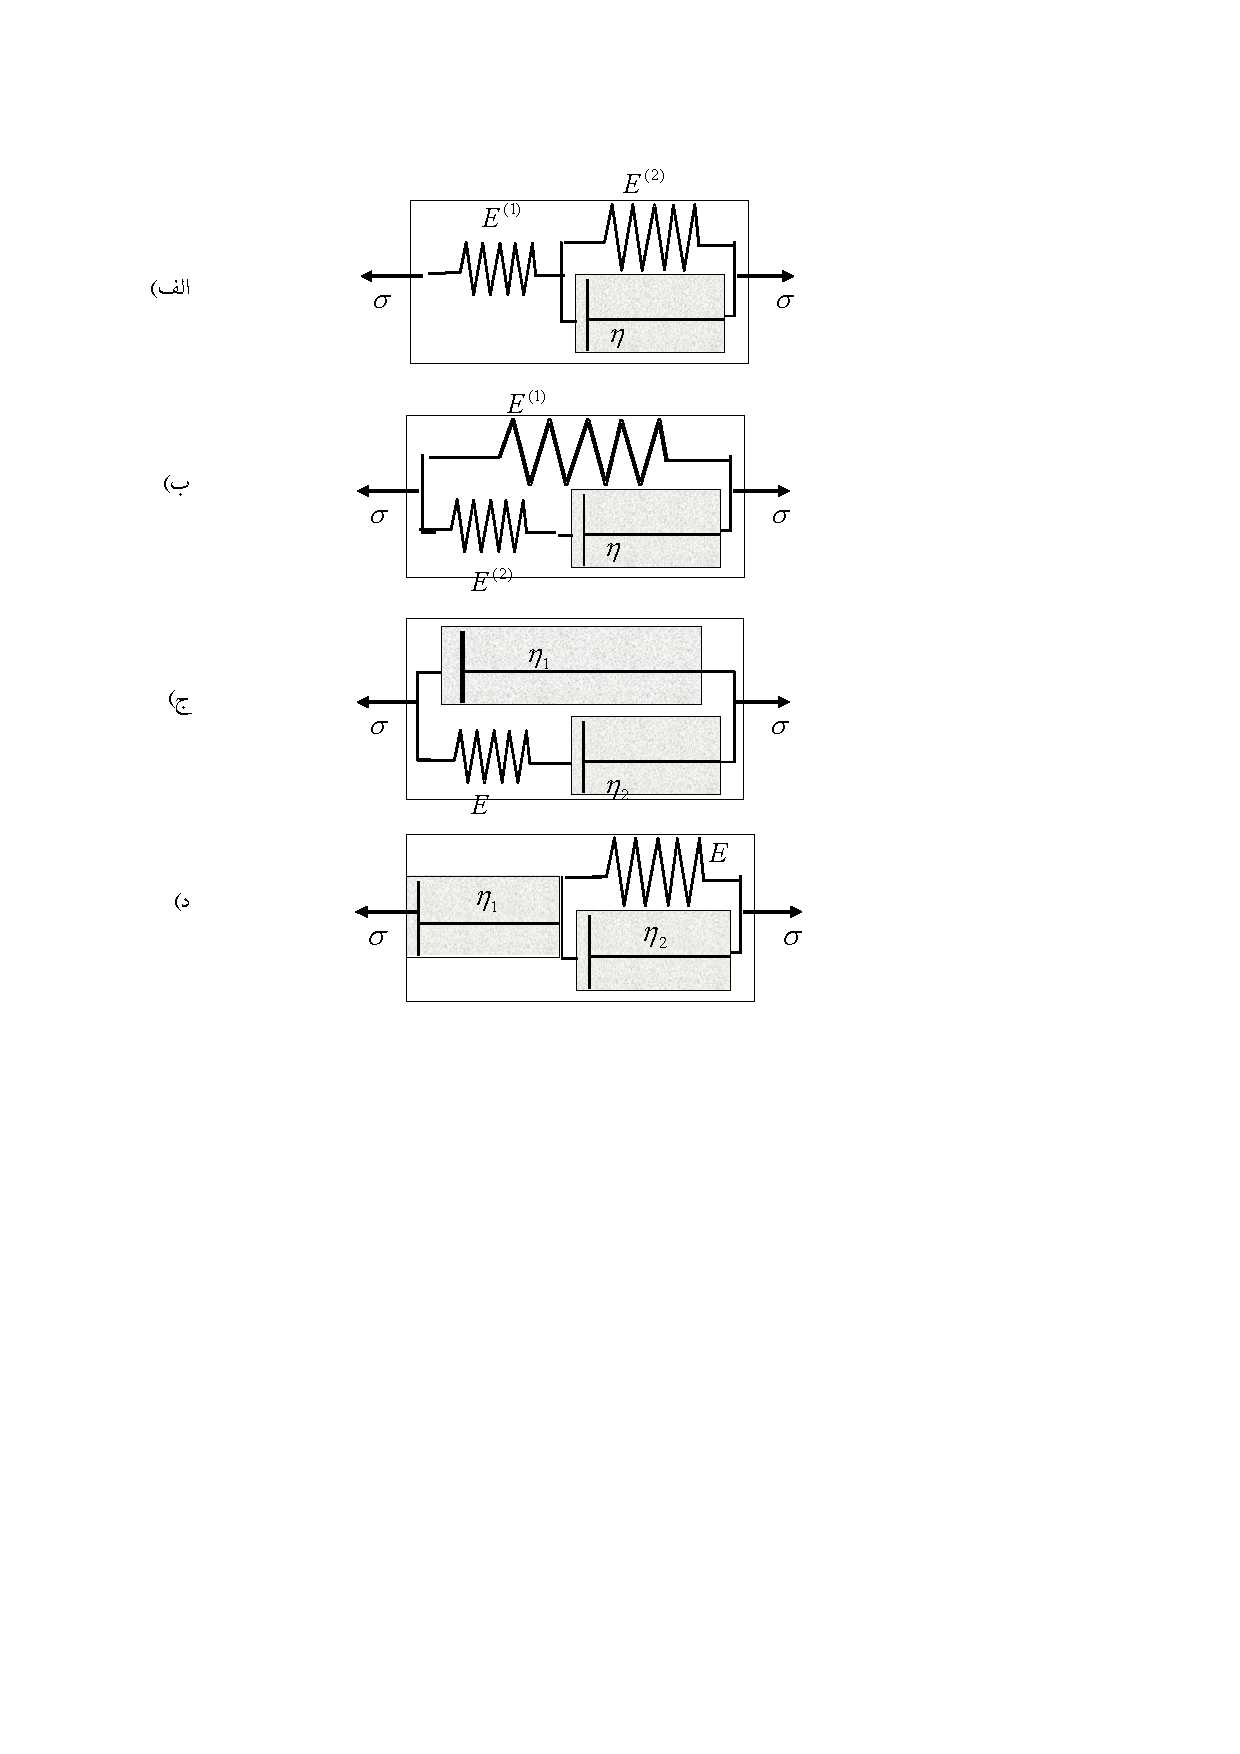
\includegraphics[width=4in]{MK}
\caption{
مدل‌های ۳ عنصری را نشان می‌دهد. الف) جامد استاندارد ۱، ب) جامد استاندارد ۲، ج) شاره استاندارد ۱، و د) شاره استاندارد ۲ را نشان می‌دهد.
}
\label{fig:MK}
\end{center}
\end{figure}
در دو مدل‌ شکل \ref{fig:MK} الف و ب   تنش اولیه به فنر(ها) منتقل می‌شود و در لحظه‌ی اولیه اعمال تنش شاهد تغییر طول هستیم، در نتیجه این دو مدل برای توصیف جامدهای ویسکوالاستیک مناسب هستند. از طرفی در دو چیدمان شکل\ref{fig:MK} ج و د به علت منتقل شدن بار تنش اولیه به عناصر دش پات، این مدل‌ها شاره‌های ویسکوالستیک را به خوبی توصیف می‌کنند. روابط تنش و کرنش برشی چهار مدل نشان داده شده در شکل \ref{fig:MK} به ترتیب در معادلات زیر بیان شده‌است،

\begin{equation*}
\begin{aligned}
& \text{(الف} \quad \sigma+\frac{\eta}{G_1+G_2}\dot\sigma= \frac{G_1G_2}{G_1+G_2}\gamma+\frac{\eta G_1}{G_1+G_2}\dot\gamma\\
& \text{(ب} \quad \sigma+\frac{\eta}{G_2}\dot\sigma= G_1\gamma+\frac{\eta (G_1+G_2)}{G_2}\dot\gamma\\
& \text{(ج} \quad \sigma+\frac{\eta_2}{G}\dot\sigma= (\eta_1+\eta_2)\dot\gamma+\frac{\eta_1\eta_2}{G}\ddot\gamma\\
& \text{(د} \quad \sigma+\frac{\eta_1+\eta_2}{G}\dot\sigma= \eta_1\dot\gamma+\frac{\eta_1\eta_2}{G}\ddot\gamma
\end{aligned}
\end{equation*}


\subsubsection{مدول واحلش مختلط}
یکی از روش‌های تعیین گرانروی خطی مواد محاسبه پاسخ تنش به کرنش نوسانی‌ است. فرض کنید که ابزارهای شکل \ref{fig:rheo} کرنش نوسانی زیر را در ماده ایجاد کنند،

\begin{equation}
\gamma(t)=\gamma_0\cos\omega t.
\end{equation}
با جایگذاری در معادله \ref{eq:sigma} داریم،
\begin{equation}
\begin{aligned}
\sigma(t)=-\int_{-\infty}^tdt'G(t-t')\gamma_0\omega\sin\omega t\\
	      =-\int_0^\infty dt'G(t')\gamma_0\omega\sin\omega (t-t')\\
	      =\gamma_0\left[G'(\omega)\cos\omega t-G''(\omega)\sin\omega t\right]
\end{aligned}
\end{equation}
که در معادله فوق،
\begin{equation}
G'(\omega)=\omega\int_0^\infty dt\sin\omega t G(t)
\end{equation}
\begin{equation}
G''(\omega)=\omega\int_0^\infty dt\cos\omega t G(t)
\end{equation}
در نتیجه می‌توان تبدیل فوریه $G(t)$ را با $G^*(\omega)$ نشان می‌دهیم و به این صورت تعریف می‌شود،
\begin{equation}
G^*(\omega)=i\omega\int_0^\infty dtG(t)e^{-i\omega t}
\end{equation}
به عبارتی دیگر، 

\begin{equation}
G^*(\omega)=G'(\omega)+iG''(\omega).
\label{eq:g*}
\end{equation}
و  $G*(\omega)$ را مدول مختلط می‌نامیم. در این مسئله $G'(t)$  مدول ذخیره‌ای\LTRfootnote{Storage modulus} است که پاسخ الاستیک ماده و $G''(t)$ مدول از دست رفته\LTRfootnote{Loss modulus} است که پاسخ گرانروی سیستم را نشان می‌دهد. مواد ویسکوالاستیک ترکیبی از رفتار‌ شاره و جامد را از خود نشان می‌دهند. یکی از روش‌های تعیین اینکه ماده جامد است یا شاره نگاه کردن به مدول مختلط در فرکانس‌های کوچک است. فرض کنید که مدول مختلط به شکل زیر باشد.
\begin{equation}
G(t)=G_e+Ge^{-\tau/t}
\label{eq:sa}
\end{equation}

در معادله \ref{eq:sa} $G_e$ مدول تعادلی است که برای شاره‌‌ی ویسکوالستیک صفر است (شکل \ref{fig:relax}). در نتیجه می‌توان مدول مختلط را می‌توان به شلک زیر نوشت،
\begin{equation}
\begin{aligned}
G'(\omega)=G_e+G\frac{(\omega\tau)^2}{1+(\omega\tau)^2}
G''(\omega)=G\frac{\omega\tau}{1+(\omega\tau)^2}
\label{eq:saG}
\end{aligned}
\end{equation}
برای محاسبه‌ی معالدلات \ref{eq:saG} از بست زیر استفاده شده‌است،

\begin{equation}
\begin{aligned}
\int_0^\infty dte^{-\omega t}=\lim_{s\rightarrow0}\int_0^\infty dte^{-\omega t-st}\\
=\lim_{s\rightarrow0}\frac{1}{s+i\omega}=\frac{1}{s+i\omega}
\label{eq:saG}
\end{aligned}
\end{equation}
پس برای فرکانس‌های کوچک مدول مختلط به شکل زیر خواهد بود،

\begin{equation}
\begin{aligned}
G^*(\omega)=
  \begin{cases}
    G_e       & \text{برای جامد ویسکوالاستیک}\\
    i\omega G\tau=i\omega\eta_0       & \text{برای شاره ویسکوالاستیک}
  \end{cases}
\end{aligned}
\end{equation}

\begin{figure}[htbp]
\begin{center}
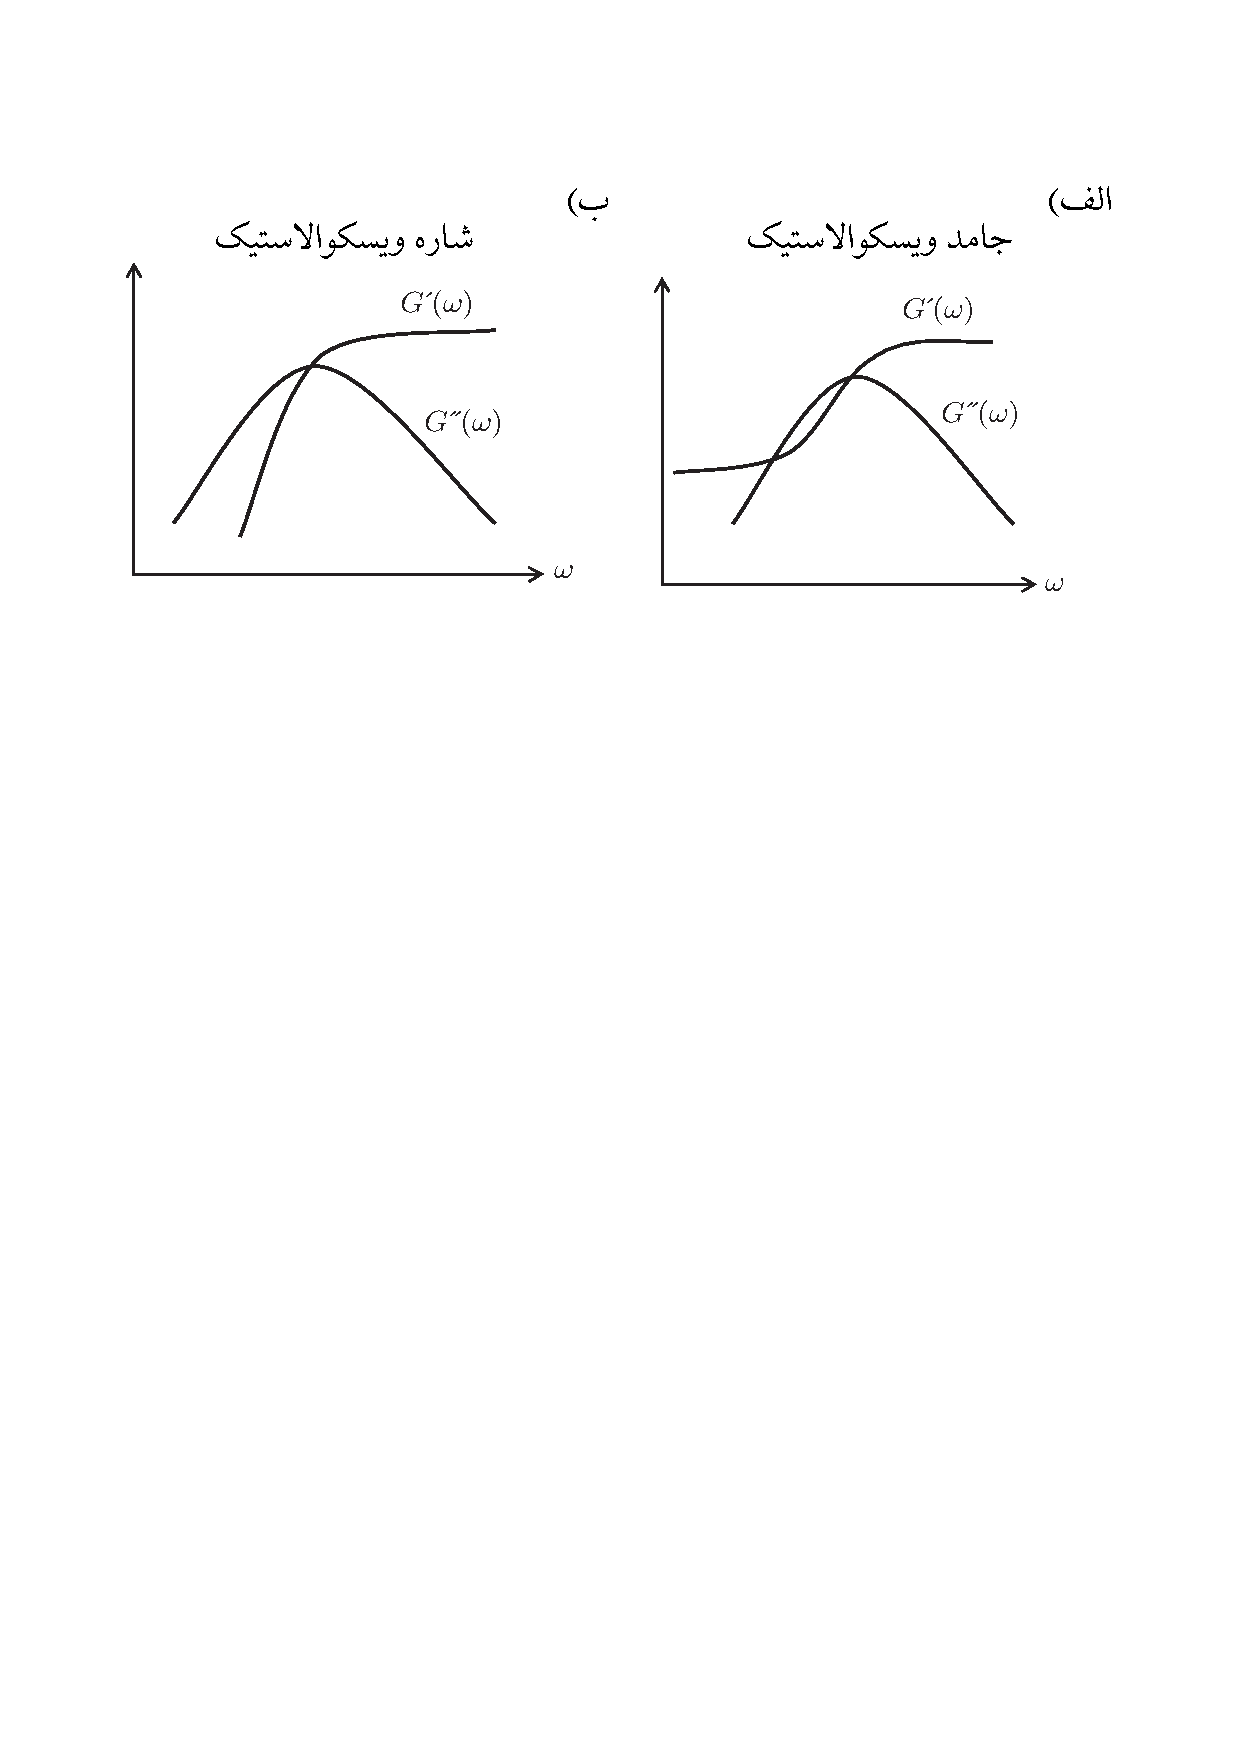
\includegraphics[width=5in]{9_4}
\caption{
رفتار عمومی عناصر مدول مختلط مواد ویسکوالاستیک را برای الف)جامد ویسکوالاستیک و ب) شاره ویسکوالاستیک نشان می‌دهد.
}
\label{fig:viscoSF}
\end{center}
\end{figure}
رفتار عمومی $G'(\omega)$ و $G''(\omega)$ در شکل \ref{fig:viscoSF} نمایش داده شده است. آزمایش‌‌های متعددی مشابه این رفتار‌ها را در شبکه‌های اکتینی موجود در سلول‌های زنده را نیز تایید می‌کند.





\subsubsection{بررسی رئولوژی غشا و اکتین}\label{lab:GG}

شکل \ref{fig:gg} مدول ذخیره‌ای و از دست رفته را برای یک شبکه اکتین ۳ بعدی (شکل \ref{fig:gg}.الف) و یک غشا که با دو چگالی مختلف پروتئین متصل کننده (شکل \ref{fig:gg}.ب و شکل \ref{fig:gg}.ج) به شبکه اکتینی متصل شده‌است را  نشان می‌دهد\cite{doi:10.1021/acs.jpcb.7b11491}. ۳ رژیم مشخص در پاسخ هر یک از این  شبکه‌ها به تنش خارجی دیده می‌شود. در شکل \ref{fig:gg} در ناحیه ۱  $G'>G''$ که نشان از این است که رفتار الاستیکی شبکه در فرکانس‌های میانی غالب است. در ناحیه ۲ رفتار توانی با نمای $0.75$ مشاهده می‌شود که با رفتار تک فیلامنتی منطبق است. و در نهایت در ناحیه ۳ رفتار ماده در فرکانس‌های پایین را می‌بینیم. در ناحیه ۳ ضریب پخش فیلامنت‌ها و ساز و کارهای مولکولی هنگام تغییر فاصله و زاویه پیوند‌های کوالانسی اهمیت دارند. مشابه این ۳ رژیم در آزمایش‌های مربوط به لایه‌ی اکتین-غشایی نیز دیده می‌شود (شکل \ref{fig:gg}.ب و ج). 

در هر ۳ آزمایش دیده‌ شده‌است که در ناحیه ۱، که مربوط به فرکانس‌های میانی است، پاسخ الاستیک ($G'$) بیشترین سهم را دارد و هنگامی‌ که شبکه اکتینی به غشا متصل می‌شود (شکل \ref{fig:gg}.ب و شکل \ref{fig:gg}.ج) ضریب الاستیک افزایش می‌یابد. سختی الاستیکی شبکه‌ی پلیمری وابسته به تعداد اتصالت میان پلیمیر هاست. از آنجایی که اتصال به غشا باعث افزایش اتصالت پلیمری می‌شود اختلاف سختی بین شکل \ref{fig:gg}.ب و ج را می‌توان ناشی از افزایش چگالی پروتئین‌های متصل کننده به غشا دانست\cite{doi:10.1021/acs.jpcb.7b11491}.

در ناحیه ۳، که مربوط به فرکانس‌های پایین است، دیده‌ شده که شبکه‌های اکتینی نسبت به تنش‌های خارجی مقاومت زیادی نشان نمی‌دهند. در تنش‌های با فرکانس پایین فیلامنت‌ها زمان کافی برای حرکت و پخش\LTRfootnote{Difussion} در راستای تنش دارند و نقاط اتصال درون شبکه‌ای با این ساز و کار تغییر می‌کند (مدل خزیدن پلیمر‌ها\LTRfootnote{Reptation modul}). فضای در اختیار پلیمر‌ها برای واحلش در مدل خزیدن به طول پلیمر‌ها وابسته است و  تغییر رژیم از ۳ به  ۱ توسط این طول تعیین می‌شود. برای شکل\ref{fig:gg}الف طول متوسط واحلش $16\mu m$ اندازه‌گیری شده که با اندازه‌گیری آزمایشگاهی این نمونه همخوانی دارد \cite{doi:10.1021/acs.jpcb.7b11491}.



\begin{figure}[htbp]
\begin{center}
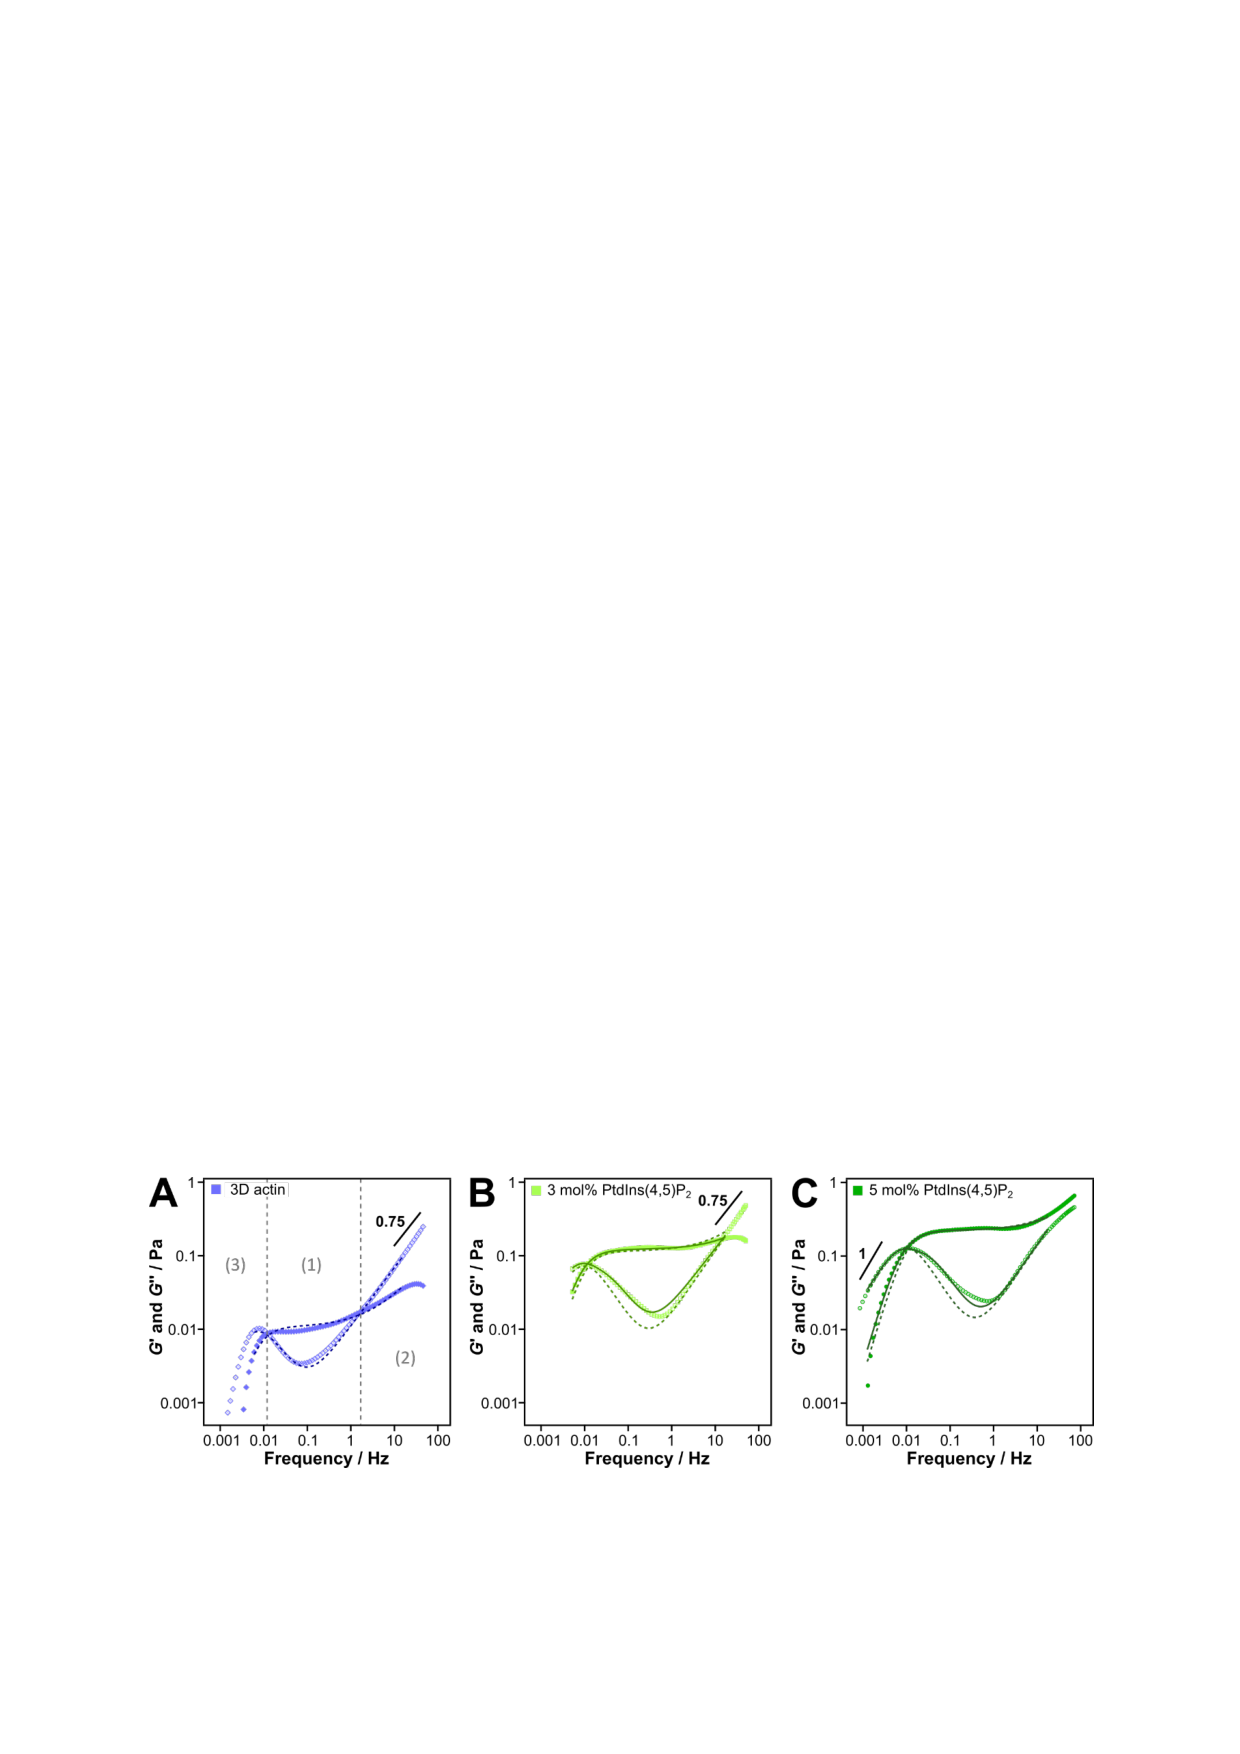
\includegraphics[width=6.5in]{GGprime}
\caption{
مشخصات ویسکوالاستیک وابسته به فرکانس لایه اکتین غشایی را نشان می‌دهد. در نمودارها مدول ذخیرا‌ه‌ای $G'$ با نقاط تو خالی و مدول از دست رفته $G''$ با نقاط تو پر نمایش داده شده‌است. خطوط مقطع  مربوط به برازش فیلامنت‌هایی است که برای توصیف آن تنها از یک زمان واحلش می‌توان استفاده کرد (ماکسول تک عنصری معادلات \ref{eq:g'} و \ref{eq:g''}). خطوط پیوسته مربوط به برازش شبکه‌ایست که با ۲ زمان‌های واحلش مشخص می‌شود (ماکسول دو عنصری معادلات \ref{eq:g'2} و \ref{eq:g''2}). شکل الف) شبکه اف-اکتین ۳ بعدی را نشان می‌دهد. ب) و ج) شبکه اف-اکتینی استکه بوسیله ازرین (Ezrin) به یک غشای لیپیدی متصل شده است و غلظت نقاط اتصال بین شبکه اف-اکتین و غشا در ب) ۳ مول٪ و در ج) ۵ مول٪ است.  خط سیاه ضخیم در الف) و ب) رفتار توانی با نمای $0.75$  و در ج) وابستگی در فرکانس‌های کم با نمای ۱ را مشخص می‌کند. برای مدلی که تنها یک  زمان واحلش (خط مقطع) دارد با رابطه‌ی $\tau=\eta/G_0$ محاسبه شده و برای الف) $\tau=139\pm15 s$، ب) $\tau=103\pm12 s$، و برای ج) $\tau=103\pm6 s$ بدست می‌آید. برای مدل دو زمانی (خط پیوسته) زمان واحلش ب) $\tau_2=28\pm4 s$، $\tau_1=121\pm9 s$ و برای ج) $\tau_2=33\pm6 s$، $\tau_1=131\pm16 s$ بدست می‌آید\cite{doi:10.1021/acs.jpcb.7b11491}.
}
\label{fig:gg}
\end{center}
\end{figure}


برای برازش داده‌های شکل  \ref{fig:gg} از مدلی که پلاگ\LTRfootnote{Plagge} و همکاران در سال ۲۰۱۶ پیشنهاد داده‌اند استفاده شده است. در این مدل فرض شده که طول اکتین‌ها بر اثر تنش تغییر نمی‌کند و تغییرات ناشی از تنش با یک پلیمر خطی که توسط یک شبکه‌ی  پلیمری موثر محاصره شده است مدل می‌شود. از آنجایی که مد‌های خمشی بسیار کم خرج‌تر از مد‌های کشسانی‌ پلیمر است در نظر نگرفتن این مدها مشکلی ایجاد نمی‌کند. در نتیجه  شبکه‌ی اکتینی که پلیمر را محاصر‌ه کرده‌است را می‌توان مانند یک راهرو فرض کرد که توسط پتانیسل‌های هارمونیک پلیمر را در درون خود هدایت می‌کند. از آنجایی که تنش‌های خارجی بر طول پلیمر اثر ندارد تنش‌ها به شکل پتانسیل داخل راهروی شبکه ظاهر می‌شود. از طرفی فرض می‌شود که شبکه‌ی اطراف پلیمر تنها از نقاط اتصال می‌توانند بر پلیمر تاثیر بگذارند \cite{doi:10.1063/1.5030169, PhysRevE.93.062502}. انرژی اتصال این پلیمر‌ها از مرتبه‌ی بزرگی دمای محیط است و عمر موثر آنها حدود چند ثانیه ‌است.\cite{doi:10.1021/acs.jpcb.7b11491} فرض می‌شود که فیلامنت‌ها در یک پتانسیل دوره‌ای یک بعدی قرار دارند که توسط نیروی خارجی دچار اختلال شده و این اختلال باعث می‌شود که فیلامنت در یک جهت بخصوص راحت‌تر حرکت کند \cite{PhysRevE.93.062502}. اختلاف در احتمال حرکت فیلامنت به معنی وجود اسطکاک در سیستم است که با مدل دش-پات\LTRfootnote{Dashpot module} توصیف می‌شود. پس می‌توانیم رفتار این شبکه را با فنر ماکسول توصیف کنیم. اینکه چند عنصر ماکسول نیاز داریم بستگی به اتصالات بین شبکه‌ای دارد. اینکه اتصالات حاصل در هم تنیدگی فیلامنت‌ها باشد یا بوسیله‌ی یک عامل پروتئینی محکم شده باشد.


پس می‌توانیم شبکه را به صورت مدول مختلط موثر زیر بنویسیتم،
\begin{equation}
\frac{1}{G^*}=\frac{1}{G_s}+\frac{1}{i\eta\omega},
\end{equation}
که $\eta$ اصطکاک حاصل از لغزش فیلامنت‌ها بر روی یکدیگر و اتصلات موقت حاصل این حرکت را توصیف می‌کند. $G_s$ هم مدول فیلامنت به طول $L$ است که با خم‌ شدن مدهایی با عدد موج $q_n=n\pi/L$ در آن ایجاد می‌شود،


\begin{equation}
\frac{1}{G_s}=\frac{1}{G_0}\sum_n\frac{\sin^2(q_nL/2)}{(Lq_n)^4+i\omega/\omega_0}.
\label{eq:Gs}
\end{equation}


که در معادله \ref{eq:Gs} $G_0$ مدول پلاتو\LTRfootnote{Plateau}، $\omega_0$ فرکانس جهش\LTRfootnote{Cross over} به شاخه فرکانس‌های بالاتر است. در دو حد فرکانس‌های بالا و پایین قسمت‌های حقیقی و موهموی مدول به ترتیب،
\begin{equation}
\begin{aligned}
G'_s\rightarrow G_0
  \begin{cases}
    0.38\cdot\alpha_0\cdot(\omega/\omega_0)^{3/4}       & \omega\gg\omega_0\\
    1       & \omega\ll\omega_0
  \end{cases}
\end{aligned}
\end{equation}
و
\begin{equation}
\begin{aligned}
G''_s\rightarrow G_0
  \begin{cases}
    0.92\cdot\alpha_0\cdot(\omega/\omega_0)^{3/4}       & \omega\gg\omega_0\\
    \omega/\omega_0       & \omega\ll\omega_0
  \end{cases}
\end{aligned}
\end{equation}
که می‌توان به شکل زیر نوشت،
\begin{equation}
G'_s=G_0(1+0.38\cdot\alpha_0\cdot(\omega/\omega_0)^{3/4})
\end{equation}


\begin{equation}
G''_s=G_0((\omega/\omega_0)^{-1}+(0.92\cdot\alpha_0)^{-1}\cdot(\omega/\omega_0)^{-3/4})
\end{equation}
که $\alpha_0$ حاصل جمع زدن روی تمام مدهاست و اعدادی که در دو معادله ظاهر می‌شود به علت وجود $i^{3/4}$ است،
\begin{equation}
i^{3/4}=e^{i\frac{3\pi}{8}}=\sin\frac{\pi}{8}+i\cos\frac{\pi}{8}=0.38+i0.92
\end{equation}
با جداکردن قسمت‌های حقیقی و مختلط می‌توان معادلات فوق را به شکل معادله‌ی \ref{eq:R*} بدست آورد،
\begin{equation}
G'=(\eta\omega)^2\cdot\frac{G'_s}{D}
\label{eq:g'}
\end{equation}
\begin{equation}
G''=\alpha_1\eta\omega\cdot\frac{\left((G'_s)^2+G"_s(G"_s+\eta\omega)\right)}{D}
\label{eq:g''}
\end{equation}
که در معادلات فوق،
\begin{equation}
D=(G'_s)^2+(G''_s+\eta\omega)^2
\end{equation}


در نتیجه پارامتر‌هایی که شناور هستند، $G_0$، $\omega_0$، $\eta$، $\alpha_0$، و $\alpha_1$. پارامتر $\alpha_1$ فازی است که اجازه می‌دهد که قسمت حقیقی و موهومی را نسبت به یکدیگر تنظیم کنیم. در شکل \ref{gg} خطوط گسسته با توجه به معادلات \ref{eq:g', eq:g''} فیت شده‌اند. زمان مشخصه‌ی ایجاد و فنای اتصالات بین فیلامنت‌ها با $\tau=\eta/G_0$ مشخص می‌شود. در مدل اتصال دائمی‌ فیلامنت به شبکه در نظر گرفته نشده‌است، در نتیجه، این مدل برای فرکانس‌های پایین رفتار فیلامنتی که قادر به پخش\LTRfootnote{Diffusion} است، برای فرکانس‌های میانی فیلامنت با اتصالات موقت، و در فرکانس‌های بالا رفتار تک فیلامنت را به خوبی توصیف می‌کند. در شکل \ref{fig:gg}ب و ج مشاهده می‌شود که رفتار شبکه اکتین متصل به غشا را نمی‌توان تنها با یک زمان مشخصه توضیح داد. اگر فرض کنیم که یک عنصر ماکسولی دیگر نیز به شبکه اضافه شده،
\begin{equation}
G'=G'_1+\alpha_3\cdot G'_2
\label{eq:g'2}
\end{equation}
و
\begin{equation}
G''=G''_1+\alpha_2\cdot G''_2.
\label{eq:g''2}
\end{equation}
از آنجایی که در هر دو شکل شاهد ناحیه پلاتو دوم نیستیم، انتظار می‌رود که ضریب مدول ذخیره‌ای دوم بسیار کوچکتر از مدول تلف باشد، $\alpha_3\ll\alpha_2$. نکته مهم این است که مشخص شده‌است که هنگام اتصال به غشا پ معرفی پروتئین‌های واصل، زمان مشخصه‌ی جدیدی به سیستم وارد می‌شود که مانند عنصر دوم ماکسول عمل می‌کند. برای این آزمایش بخصوص زمان مشخصه دوم که مربوط به اتصال پروتئین ازرین\LTRfootnote{Ezrin} است، $\tau=0.03 s^{-1}$ گزارش شده‌است. \cite{doi:10.1021/acs.jpcb.7b11491}

\subsection{هسته}\label{lab:nucleus}

\subsubsection{نقشه برداری از برهمکنش‌های کروماتین‌ها}
نحوه‌ی تا شدن کروموزم‌ها داخل هسته اطلاعات زیادی در مورد ساختار کروموزوم در اختیار ما قرار می‌دهد. این اطلاعات می‌تواند نشانه‌ی از سازوکار فعالیت ژن‌ها\LTRfootnote{أGene Activity} و به طور کلی وضعیت هسته در اختیار ما قرار دهد. با روش های-سی\LTRfootnote{Hi-C} \cite{Lieberman-Aiden289} می‌توان برهمکنش ژن‌ها را در داخل هسته دنبال کرد. به طور خلاصه در این روش قسمت‌های مختلف کروماتین  علامت گذاری می‌شود.  ماتیریسی شکل \ref{fig:Hi-C} یکی از نتایج این آزمایش را نشان می‌دهد. رشته‌ی کروموزوم به مناطق یک میلیون جفت بازی\LTRfootnote{Mega Basepare} ($1MB$)  تقسیم می شود که به آن لوکس\LTRfootnote{Locus} گفته می‌شود. هر عضو ماتریس $M$، $m_{ij}$  تعداد اتصالات بین لوکی\LTRfootnote{Loci} (جمع لوکس) $i$ و $j$ را مشخص می‌کند.
\begin{figure}[htbp]
\begin{center}
\includegraphics[width=3.5in]{Hi_C}
\caption{
  قسمتی از ماتریس اتصال مربوط به کروموزم ۱۴ را نشان می‌دهد. هر پیکسل وضعیت اتصال یک لوکس $۱MB$ با یک لوکس $1MB$ دیگر را نشان می‌دهد. شدت رنگ مشخص کننده تعداد اتصالات بین دو لوکس است. خطوط روی محورها به فواصل $۱۰MB$ رسم شده‌است \cite{Lieberman-Aiden289}.
}
\label{fig:Hi-C}
\end{center}
\end{figure}



مطالعه ماتریس اتصال نشان می‌دهد که در طول کروموزم نواحی متشکل از لوکی‌های زیادی وجود دارد که یا علاقه به ایجاد اتصال زیاد با نواحی دیگر دارند یا اتصالات کمتری ایجاد می‌کنند. این نواحی  به طور عمومی‌ با دو دسته لوکی تقسیم بندی می‌شود، لوکی $A$ دارای نواحی با اتصالات کم و لوکی $B$ با اتصالات زیاد است. وجود اتصالات زیاد در ناحیه $B$ خبر از این می‌دهد که در این ناحیه کروموزم بیشتر پَک\LTRfootnote{Pack}  شده‌است. به عبارت دیگر ژن‌هایی که در نواحی نوع $B$ قرار دارد علاقه‌ی بیشتری به چیدمان‌های فضایی نزدیک به هم دارند. همچنین نتایج آزمایش‌ فیش سه بعدی\LTRfootnote{3D-FISH} نیز تایید می‌کند که قسمت‌هایی از کروماتین که در نواحی مشابه قرار دارند ($A$ یا $B$) در نزدیکی یکدیگر ظاهر می‌شوند. 
\begin{figure}[htbp]
\begin{center}
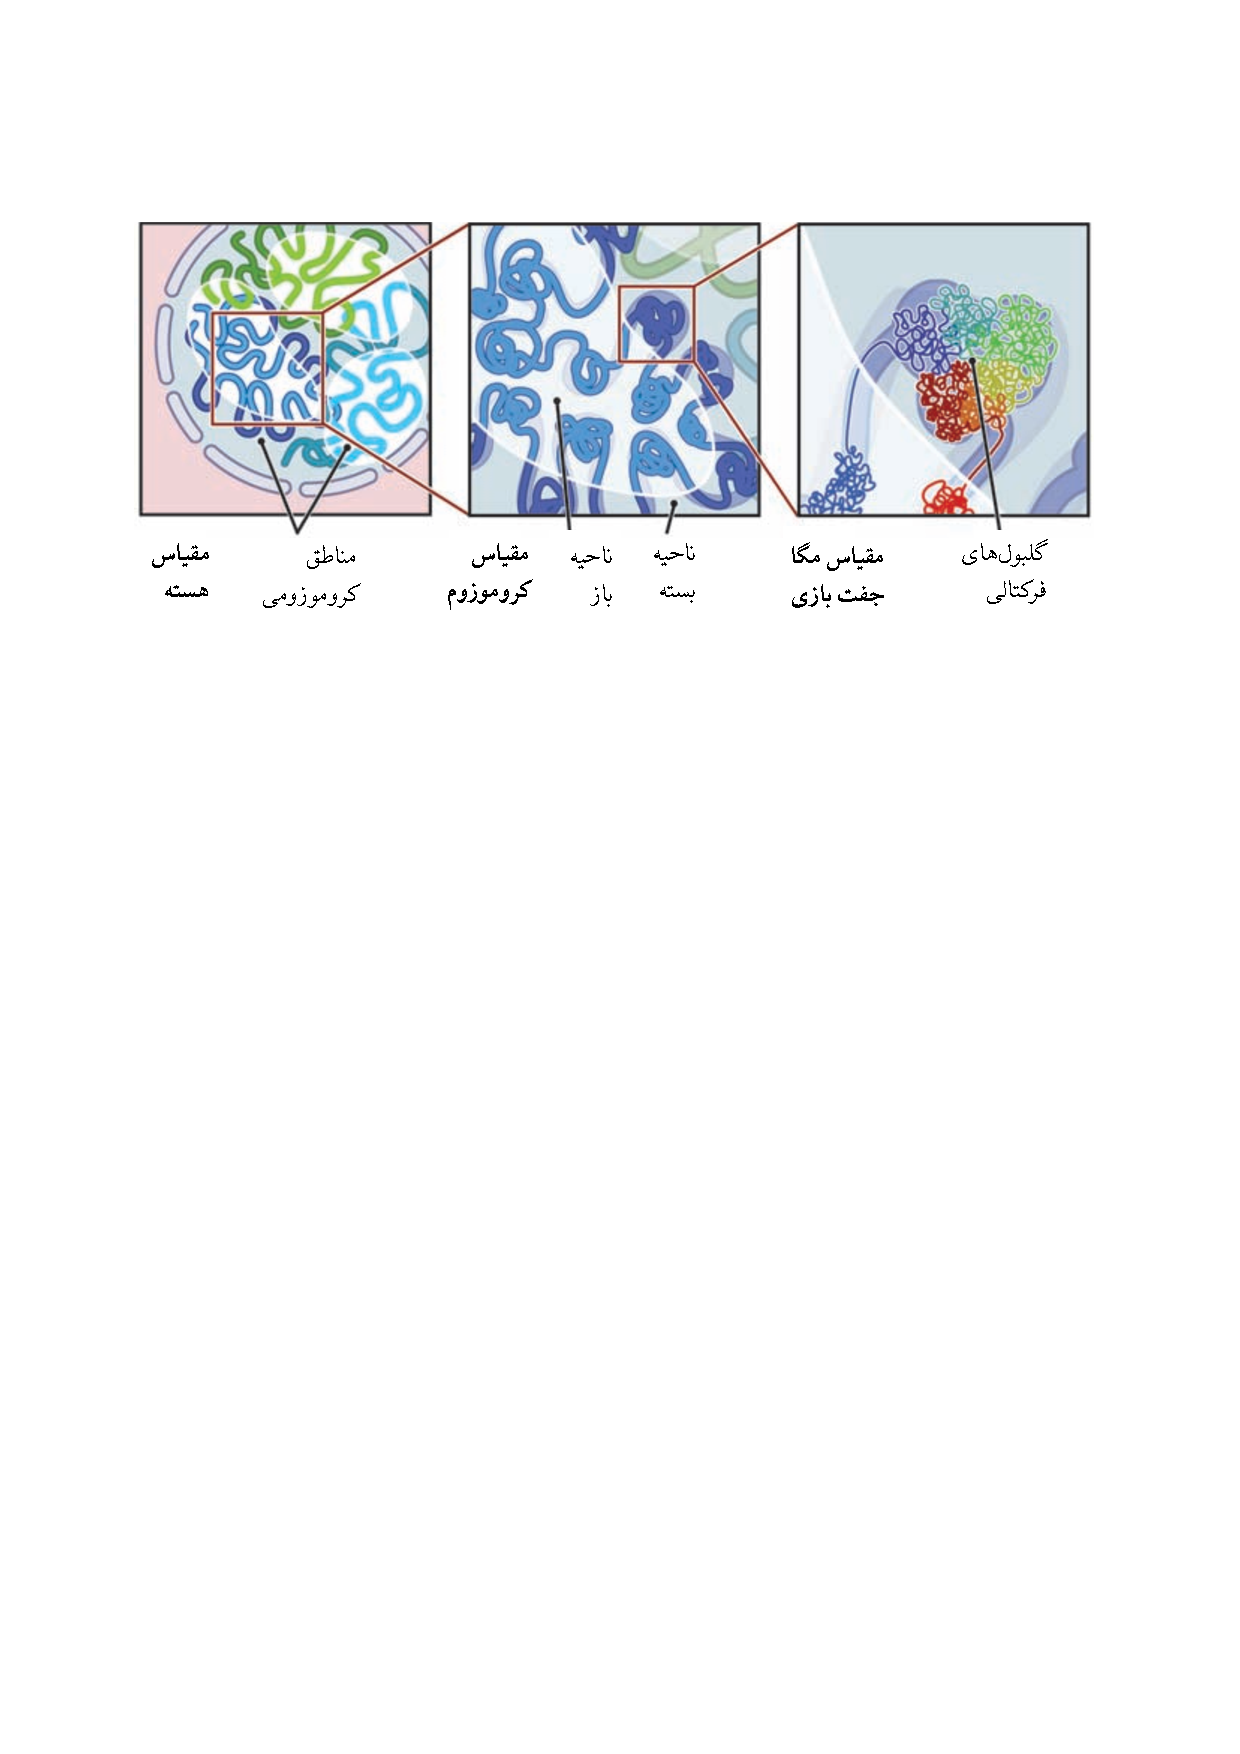
\includegraphics[width=4.5in]{chromatin_coarse_grained}
\caption{
 معماری کروماتین را در ۳ مقیاس مختلف نشان می‌دهد. در شکل بالا کروموزوم‌ها را نشان می‌دهد که هر کدام در فضا‌های جدا و مشخص قرار دارند. در شکل وسط نواحی باز و بسته را نشان می‌دهد که رشته‌ی کروماتین از میان این نواحی می‌گذرد. و در شکل پایین رفتار کروماتین را در مقیاس یک میلیون جفت بازی می‌بینیم که به صورت گلبول فرکتالی رفتار می‌کند \cite{Lieberman-Aiden289}.
}
\label{fig:chromo_coarse}
\end{center}
\end{figure}

\subsubsection{ساز و کار کروماتین در هسته }
در حال حاضر تصور ما از کروموزوم‌های داخل هسته‌ی سلول‌ها آرایشی به دور از رشته‌های در هم تنیده‌ی نامنظم است \cite{Gibcus:2013fj,Lieberman-Aiden289}. در این بخش علاقه داریم که نظم این سیستم در هم‌تنیده‌ و پیچیده‌ را در مقیاس بزرگ یعنی در مقیاس میلیون جفت بازی\LTRfootnote{Mega Basepare} مطالعه کنیم. یکی از مدل‌ها درشت دانه برای توصیف رفتار گزارش شده توسط آزمایش های-سی  مدل درشت‌ دانه‌ی پیشنهاد شده توسط \cite{Lieberman-Aiden289} است که در شکل \ref{fig:chromo_coarse} نشان داده شده‌است. در این مدل کروماتین رشته‌ی بلندی درون هسته در نظر گرفته می‌شود که از دو عنصر $A$ و $B$ تشکیل شده‌است.   در این مقیاس کروماتین در فضاهای مشخصی قرار دارد\cite{Gibcus:2013fj,Lieberman-Aiden289}. همچنین نتایج اندازه‌گیری با روش‌های های-سی و تصویر برداری از لوکی‌ها تایید می‌کند که نواحی هم نوع ($A$ و $B$) علاقه دارند که با یکدیگر برهمکنش داشته باشند. در مقیاس پیشنهاد شده  ساز و کار فشرده شدن کروماتین وجود پروتئین‌هایی شبیه به کوهسین\LTRfootnote{Cohesin} است که که به شکل حلقه بوده و می‌توانند روی DNA حرکت کنند و طی فرآیندی حلقه‌ ایجاد کنند\cite{Nuebler196261}. شکل \ref{fig:TADloops} این مدل را نشان می‌دهد.

\begin{figure}[htbp]
\begin{center}
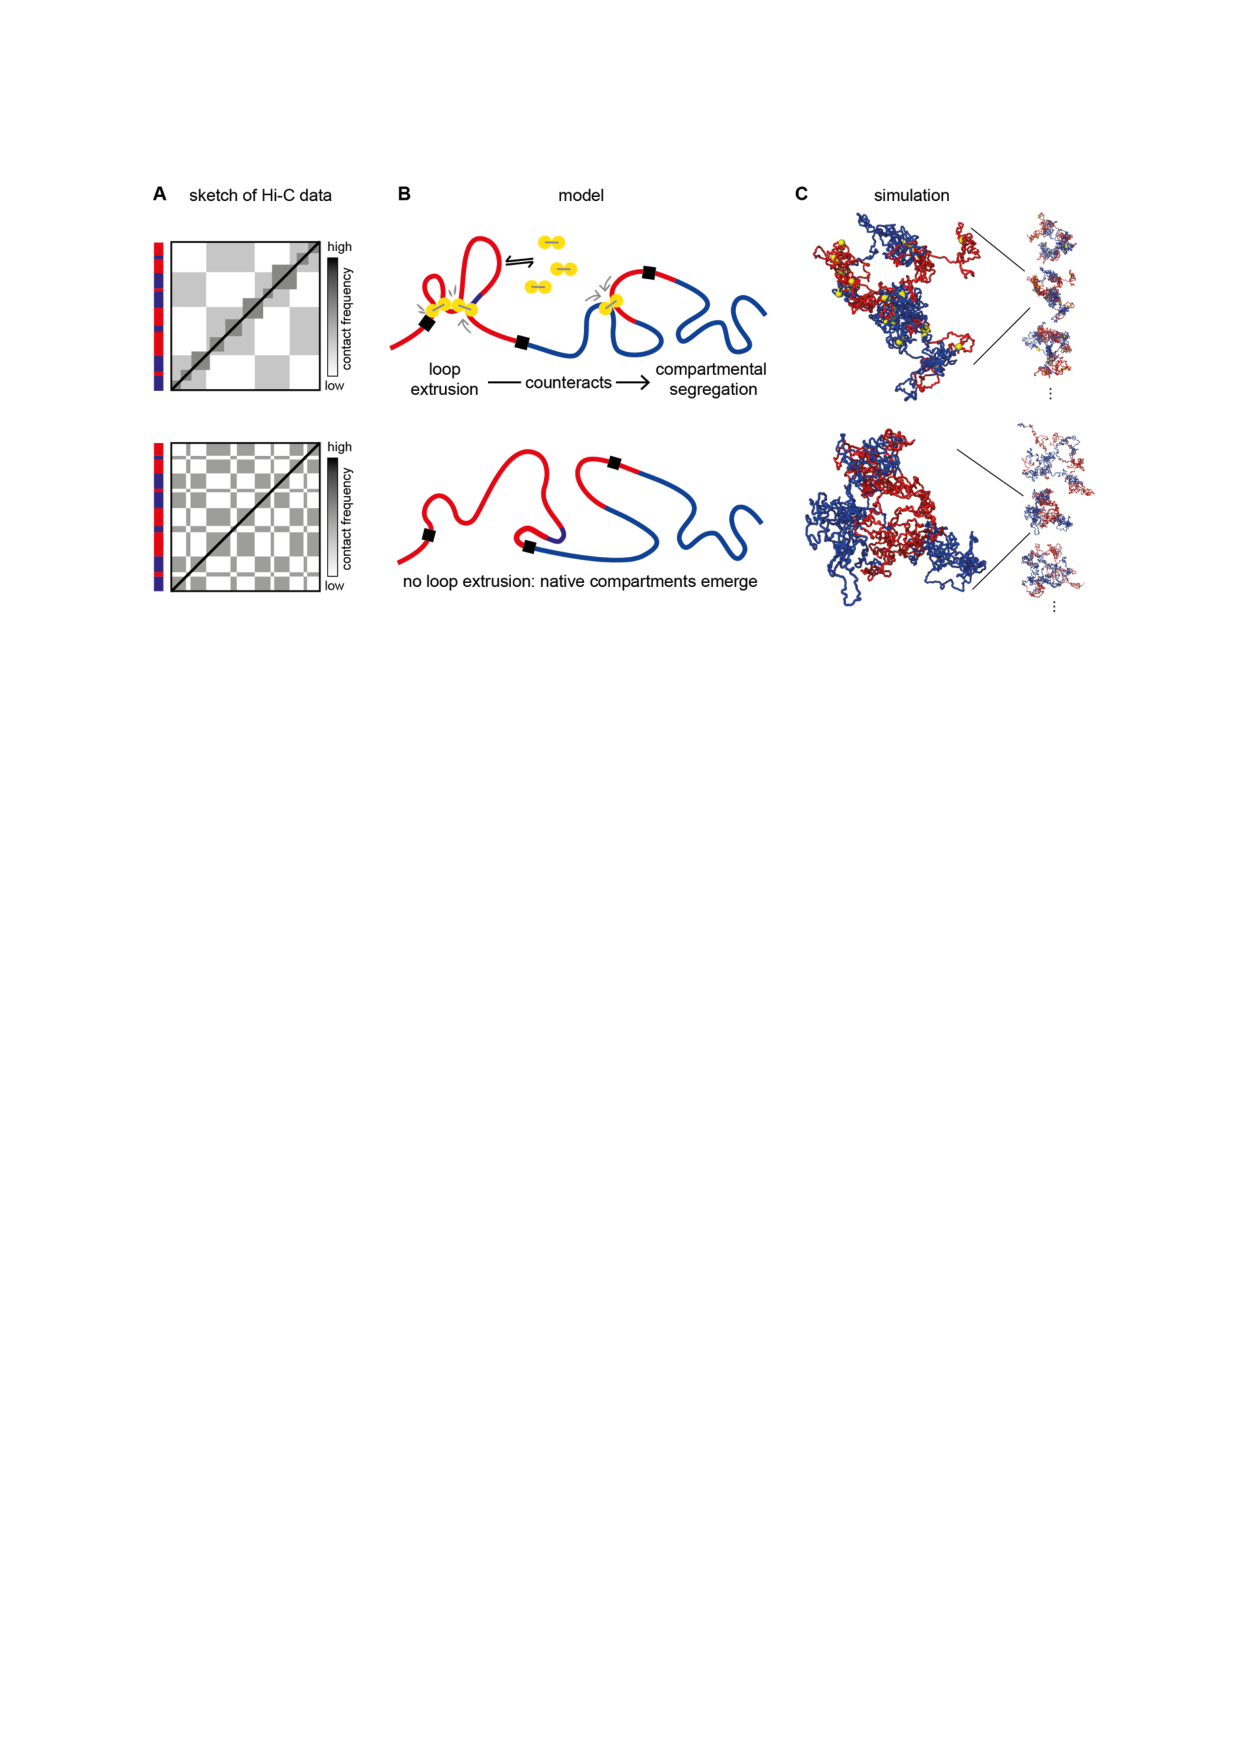
\includegraphics[width=5.5in]{TAD_loops}
\caption{
ردیف اول مدل ایجاد حلقه و ردیف پایین مدل جدا شدن ناحیه‌ها در طول کروماتین را مشخص می‌کند. الف) شکل کارتونی  الگو ایجاد شده توسط مدل ایجاد حلقه‌ را نشان می‌دهد. این الگو به شکل مربع‌های نشان دهنده نواحی با احتمال اتصال بالا در راستای قطر نقشه‌ ظاهر می‌شود. از طرفی مدل تقسیم بندی فضایی کروماتین به نواحی $A$ و $B$ الگویی شطرنجی دارد. نقشه‌ی مدل ایجاد حلقه بر روی کروماتین را نشان می‌دهد. این پروتئین‌ها با مصرف $ATP$ قادر به ایجاد حلقه در $DNA$ هستند. ب) نشان می‌دهد که در حضور فاکتورهای ایجاد کننده‌ی حلقه الگوی حلقه‌ها  و در عدم حضور حلقه‌ها الگوهای شطرنجی خواهیم داشت. ج) قسمتی از شبیه‌سازی به طوب ۱۰ میلیون جفت بازی را برای هر مدل نشان می‌دهد.
}
\label{fig:TADloops}
\end{center}
\end{figure}

فرآیند ایجاد نواحی مجزای $A$ و $B$ در طول کروماتین با مدل حلقه قابل توضیح نیست. همانطور که در شکل \ref{fig:TADloops} ردیف پایین مشاهده می‌کنید، الگوی ایجاد شده توسط اتصالات لوکی‌ها در کروموزوم الگوی صفحه شطرنجی تشکیل می‌دهد. این الگو نشان می‌دهد که بخش‌هایی بر روی کروماتین با بخش‌های دیگری احتمال اتصال زیاد و با بخش‌هایی دیگر احتمال اتصال کمی دارند. از آنجایی که توزیع بخش‌های اتصال زیاد همیشه در همسایگی نزدیک آنها قرار \textbf{ندارد} الگوی شطرنجی پدید می‌آید. اما زمانی که اتصال با فرآیند ایجاد حلقه در کروماتین ایجاد ‌شود اتصالات بسیار موضعی‌است در نتیجه الگوی مربع شکل در امتداد قطر ماتریس اتصال ایجاد می‌شود (شکل\ref{fig:TADloops} ردیف بالا).
 
 یکی از مدل‌های محبوب پیشنهادِ وجود برهمکنش‌های مشخص بین نواحی است که بر اثر جدا سازی فازی قسمت‌های هم نوع در فضاهای مشخص در کنار یکدیگر قرار می‌گیرند \cite{Nuebler196261}. این نواحی با رشته‌های پلیمری مدل می‌شوند که بر روی‌ آن قسمت بندی‌های زیادی از ۲ نوع ناحیه ایجاد شده است و هر لوکی می‌تواند نوع $A$ یا $B$ باشد. این دو نوع ناحیه از لحاظ اندازه و خواص الاستیکی با یکدیگر مشابه‌اند ولی به لحاظ برهمکنش متفاوت هستند.  یعنی برای برهمکنشهای $A-A$، $B-B$، و $A-B$ انرژی مختلفی تعریف می‌شود. برای جدا سازی مناطق با محاسبه انرژی برهم کنش‌ها به هر منطقه برچسب کلی $A$ یا $B$ داده می‌شود. همچنین بین لوکی‌ها نیروی دافعه وجود دارد تا لوکی‌ها در داخل یکدیگر فرو نروند.
شبیه‌سازی همچنین نشان می‌دهد که افزایش تعداد عناصر ایجاد حلقه در کروماتین‌ها با ایجاد ناحیه‌های $A$ و $B$ مخالفت می‌کند \cite{Nuebler196261}.
نتیجه‌ی جدایی مناطق کروماتینی به دو ناحیه به وسیله مدل جدا سازی فازی با انرژی برهمکنش لوکی‌ها قایل تنظیم است. یعنی با نسبت‌های مختلف انرژی مناطق $B$ ممکن است در مرکز هسته  متمرکز شوند یا نزدیک به غشای هسته. از طرفی در اکثر سلول‌ها مشاهده شده است که کروماتین با غشای هسته اتصالات قوی برقرار می‌کنند و به دیواره‌ی هسته متصل می‌شوند. در نتیجه‌ برای مدل‌سازی این فرآیند پیشنهاد می‌شود که در انتهای هر کروماتین نواحی $B$ قرار دهیم (این پروتئین‌ها بیشتر مسئول اتصال به غشای هسته هستند) ولی برهمکنش با هسته نیز برای آن تعریف شود  \cite{Nuebler196261}.






%\section{
%اهمیت  پژوهش
%}

\clearpage
\section{طرح پژوهش}
\subsection{بخش اول}

بخشی از این پژوهش به توسعه و تکمیل مدل سلول مجازی\LTRfootnote{The Virtual Cell} می‌پردازد. این مدل مجموعه‌ای از مدل‌های شناخته شده و تایید شده‌ی فیزیکی است که رفتار مکانیکی اجزای مختلف سلول را توصیف می‌کند. این مدل ابزار اصلی برای پیش‌برد شبیه‌سازی این پژوهش خواهد بود. این مدل از بخش‌هایی همچون اسکلت برون سلولی، غشا، شبکه‌ی اکتینی، غشای هسته، و کروماتین‌های داخل آن تشکیل شده‌است. هر یک از بخش‌‌های نامرده نیاز به تنظیم و توسعه دارند تا این پژوهش را عملی سازند. برای مثال در راستای بررسی تاثیر هندسه و نیروی خارجی بر شکل هسته‌ی سلول و چیدمان کروماتین‌های درون آن، فرآیند انتقال و توزیع نیرو در مدل سلول مجازی توسعه پیدا خواهد کرد. \\


رفتار سلول نسبت به نیروی خارجی و هندسه‌ی محیط اطراف به عوامل مختلف زیستی، شیمیایی، و فیزیکی وابسته است. در شبیه‌سازی با مدل مجازی سلول می‌توانیم سهم فیریک مسائل را از بخش‌های دیگر جدا کنیم. به طور مثال اگر سلولی بر روی یک سطح مشخصی شروع به حرکت کند، با این مدل می‌توان فهمید که چه مقدار از این حرکت سهم کمینه‌سازی انرژی مکانیکی سلول است. \\


همچنین می‌توان به همکاری جدید بین گروه‌ ماده‌چگال نرم دکتر اجتهادی و گروه انبرک نوری دکتر سید ریحانی اشاره کرد. در این قسمت با استفاده از نتایج رئومتری گروه دکتر سید ریحانی بر روی گلبول‌های قرمز می‌توانیم مدل سلول مجازی را تصحیح و کالیبره کنیم. (اطلاعات بیشتر در بخش \ref{lab:GG})
\subsection{بخش دوم}
کروماتین حامل اطلاعات موجودات زنده‌است. از طرفی این اطلاعات به علت محدودیت فضای داخل سلول همیشه در دسترس نیستند. ساختار و چیدمان کروماتین درون سلول سهم مهمی در نحوه و شانس خوانده شدن ژن‌های بر روی آن دارد . افراد در سال‌های اخیر فناوری لازم برای مطالعه‌ی آزمایشگاهی این چیدمان را تهیه کرده‌اند (اطلاعات بیشتر در بخش \ref{lab:nucleus}). \\

در بخش دوم پژوهش از مدل تکمیل شده‌ی سلول مجازی برای بررسی هندسه‌ی اتصالات کروماتین (ماتریس اتصالات) و ساختار کروماتین‌ها در هسته‌ی سلول استفاده خواهد شد. در این پژوهش علاوه بر بررسی ساختار کروماتین‌ در حالت تعادلی سلول، با اعمال تنش به هسته‌ی سلول قادر به  بررسی پاسخ ساختار کروماتین و ماتریس اتصالات آن تحت نیرو‌های خارجی نیز هستیم.

\subsubsection{بخش تکمیلی}
مهاجرت سلول مسئله روز و جال دیگری است که در صورت مناسب بودن شرایط می‌ةوان در ادامه این پژوهش دنبال کرد. مهاجرت سلول فرآیندی غیر تعادلی است که بخش زیستی و فیزیکی آن هسته‌ی سلول را تحت تنش قرار می‌دهد و از حالت کره به بیضی تغییر می‌دهد. در صورت امکان می‌توان مدل‌های مهاجرت سلولی را در مدل سلول مجازی توسعه داد و تغییرات ساختار کروماتین و ماتریس اتصلات آن را تحت تنش‌های ناشی از فرآیند غیر تعادلی حرکت سلول نیز بررسی کرد (اطلاعات بیشتر در بخش‌های \ref{lab:skeleton}و \ref{lab:traction}  ).
%\section{برنامه پژوهشی}

text\cite{Dekker:2017rt}\cite{Tee:2015gf}\cite{Gerlitz:2011bh}\cite{Shi:2018uo}\cite{10.3389/fnins.2017.00559}\cite{Shaebani:2017xy}\cite{C6RA23012A}

\clearpage
\section{منابع}

\unsetRL
%\renewcommand{\refname}{whatever}
\bibliography{reference} 
\bibliographystyle{IEEEtran}
%\renewcommand\refname{مراجع}


	        
	       
\clearpage
\chapter{بررسی مدل‌ها شبیه‌سازی غشای سلولی}
\setRL
\clearpage
\pagenumbering{arabic} 



در این بخش تمام اطلاعات مدل‌سازی غشای لیپیدی را می‌نویسم.


\section{
بررسی مدل‌ها شبیه‌سازی غشای سلولی.
}
\subsection{
بیولوژی غشا و ساختار آن
}
\subsection{
بررسی مدل گومپر-کرول
}
همانند بخش‌های دیگر فیزیک مانند دینامیک شاره‌ها و نظریه‌ی رسانایی در فلزات، نظریه‌ی پوسته‌های نازک می‌خواهد فیزیک اختلال‌های کُند را بر حسب چند پارامتر ماکروسکوپیک بیان کند. البته که بارها نشان داده شده که چنین نظریه‌هایی به شکل‌ جالبی فروپاشی می‌کنند. مانند با توجه به نظریه جفت شدن مُود‌ها و نظریه باز به هنجارش، افت و خیز‌ها گرمایی باعث می‌شوند که وشکسانی برشی
\LTRfootnote{shear viscosity}
شاره‌های تراکم ناپذیر در ۲ بعد به صورت لوگاریتمی با افزایش اندازه سیستم به بی نهایت میل می‌کند 
\cite{gomppernelson2012}
. غیر خطی شدن رفتار در مورد پوسته‌ها و صفحه‌های نازک نیز اتفاق می‌افتد. افت و خیز گرمایی می‌توانند بر ساختار پوسته‌هایی میکرونی به شدت تاثیر بگذارند زیراکه انرژی خمشی لازم برای بیشتر تغییر شکل‌های پوسته‌های خیلی نازک که زخامت آنها در مقیاس نانومتر است، حدود $k_BT$ است که در اینجا $k_B$ ثابت بولتزمن و
$T$
دماست. مکانیک آماری غشاها و صفحات تخت در گذشته بسیار دقبق مورد مطالعه قرار گرفته. در این سیستم‌ها نشان داده شده‌است که افت و خیز گرمایی در غشاهای تخت باعث می‌شود که مدول کشسانی درون صفحه‌ای
\LTRfootnote{in-plane}
 تابع اندازه‌‌ی سیستم باشد و در اندازه‌های بزرگ به سمت صفر میل کند در حالی که مدول خمشی به بی‌نهایت میل می‌کند. این پدیده‌های ناهنجار ناشی از جفت شدگی غیر خطی میان تغییر شکل‌های خارج از صفحه‌ای (عمود بر صفحه) و تنش‌هایی داخل صفحه‌ی که ایجاد می‌کنند که هنگام تغییر شکل خارج از صفحه از مرتبه‌ی دوم هستند. حتی اطلاعات کمتری در مورد تاثیر افت و خیز گرمایی بر غشا‌های کروی موجود است (شکل 
 \ref{fig:mem1}
)
ولی جفت شدگی بین تغییر شکل‌های روی سطح و عمود بر سطح با یکدیگر تفاوت دارند. به علت وجود هندسه‌ی بسته‌ی غشاهای شبه کروی تغییر شکل حتما همراه با ایجاد کشش در سطح است. در نتیجه جابجایی عمود بر سطح به شکل جملات مرتبه‌ی اول در تنش موازی با صفحه ظاهر می‌شوند. در نتیجه جفت‌ شدگی‌های غیر خطی متفاوت با غشای تخت ایجاد می‌‌شود.

انرژی کشسانی تغییر شکل غشا به شعاع
 $R$ 
با نظریه‌ی پوسته‌های نازک کم عمق مدل‌سازی می‌شود. با این روی‌کرد صحبت از فرورفتیگی‌ها یا برآمدگی‌هایی است که نسبت به بخش مورد مطالعه کوچک هستند. جابجایی درون صفحه با فنون دو مولفه‌ای 
$u_i(\boldsymbol{x})$ 
پارمتری‌سازی شده و جابجایی‌های عمود بر سطح با میدان 
$f(\boldsymbol{x})$
در دستگاه مختصات
$\boldsymbol{x}=(x_1,x_2)$
موازی سطح تعریف می‌‌شود. ما فرض می‌کنیم که تمام غشای مورد بررسی دارای خواص کشسانی هماهنگ در همه جای سطح است در نتیجه می‌توانیم تاثیر ۱۲ نقطه نقصی که به ناچار بر روی سطح کره‌ی مثلث بندی شده ایجاد می‌شود را ناچیز در نظر بگیریم.
\subsection{میدان و تنش در نظریه پوسته‌ی کم عمق}
در این قسمت ما طبق روش کویتر
\LTRfootnote{Koiter}
و
\LTRfootnote{Heijden}
هیدن

پیش می‌‌رویم
\cite{Heijden2008WTK}
. بخشی از کره که دچار فرورفتگی کوچکی شده را در نظر می‌گیریم و دستگاه مختصات دکارتی 
$(x_1,x_2)$
را طوری تعریف می‌کنیم که در مبدا بر قسمت بدون ناهمواری از کره مماس است (شکل 
\ref{fig:nelson_figs1}
). در نتیجه مرکز کره بر روی محور 
$z$
خواهد بود. می‌توان کره را با فاصله نقاط آن از صفحه‌ی مختصات پارامتری سازی کرد:
\begin{equation}
Z(x_1,x_2) = R\left(1-\sqrt{1-\frac{x_1^2}{R^2}-\frac{x_2^2}{R^2}}\right)
\label{eq:nelsonS1}
\end{equation}
\begin{figure}[h]
\begin{center}
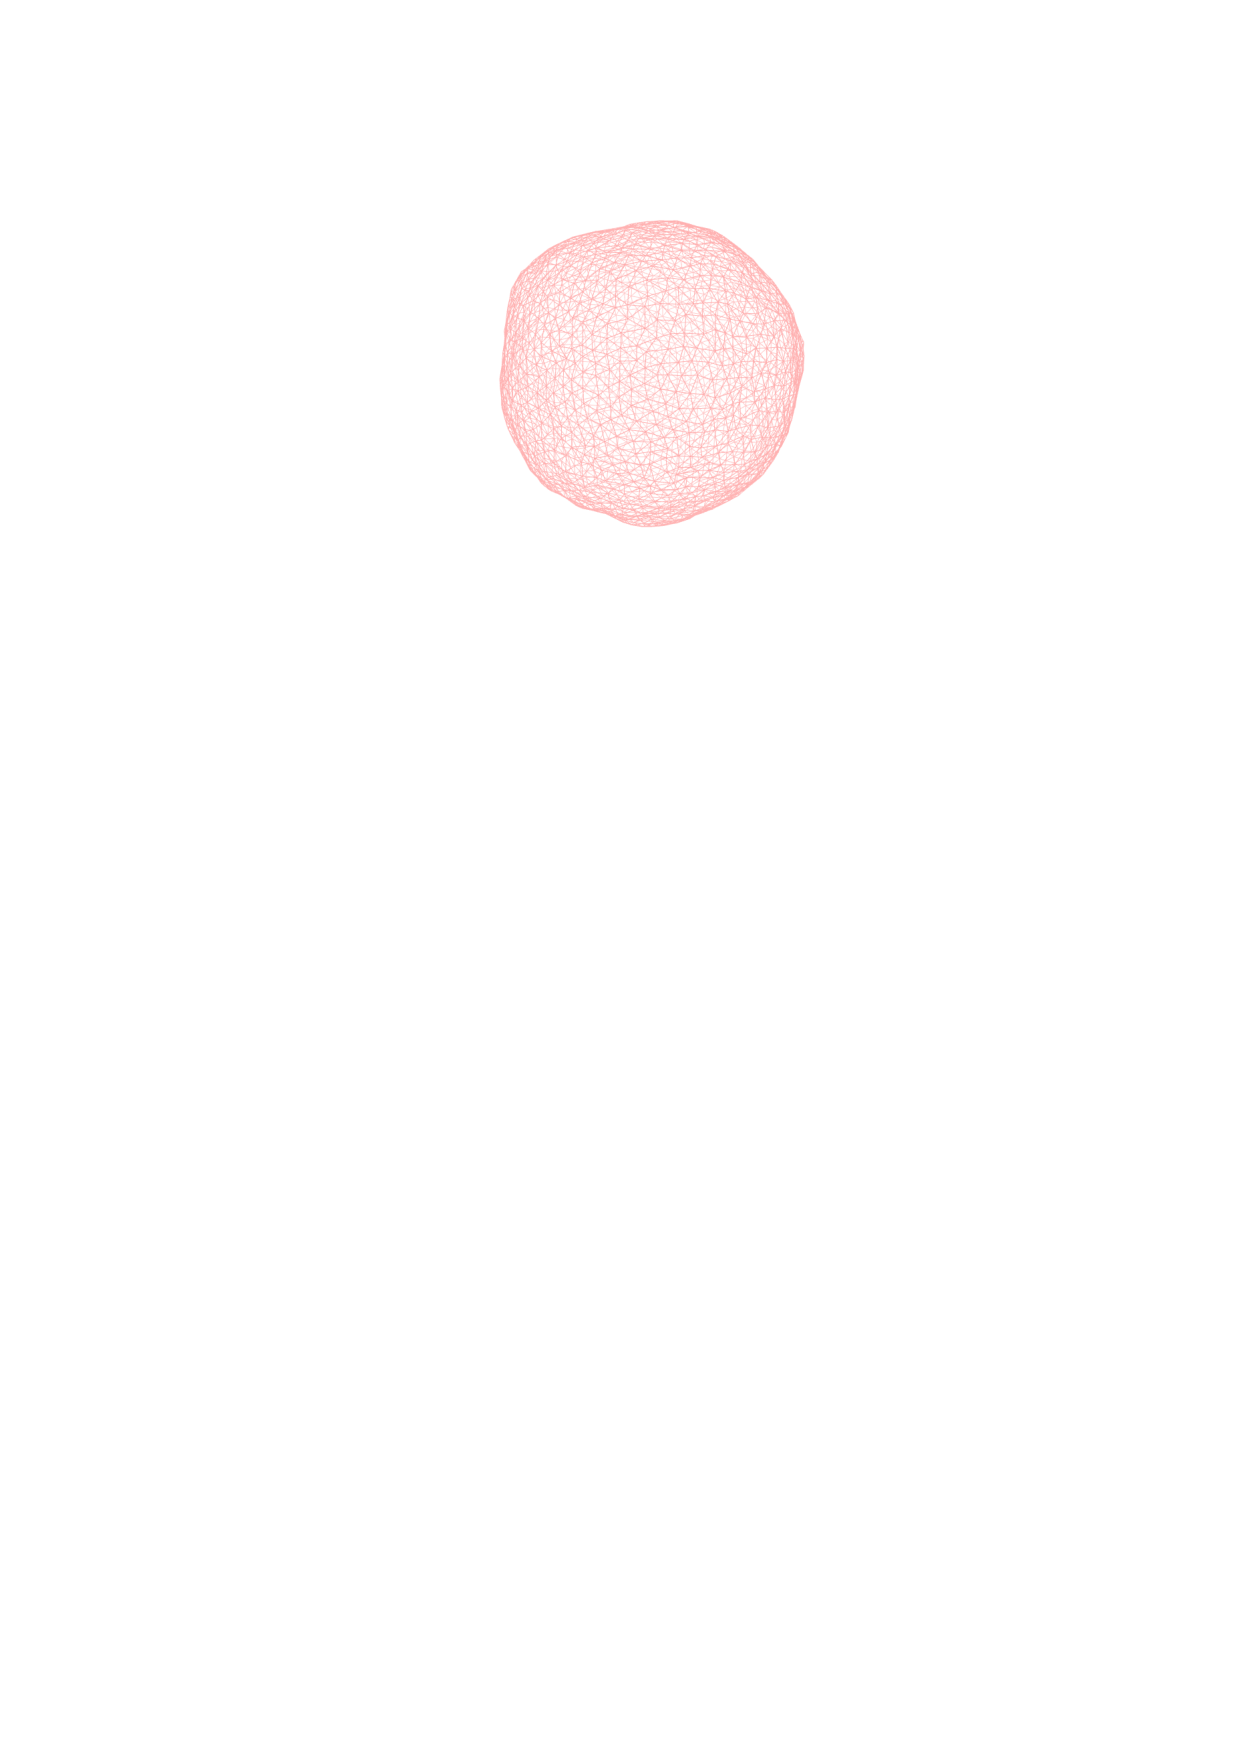
\includegraphics[width=4in]{mem_sim1}
\caption{
غشا با هندسه‌ی کروی.
}
\label{fig:mem1}
\end{center}
\end{figure}
\begin{figure}[h]
\begin{center}
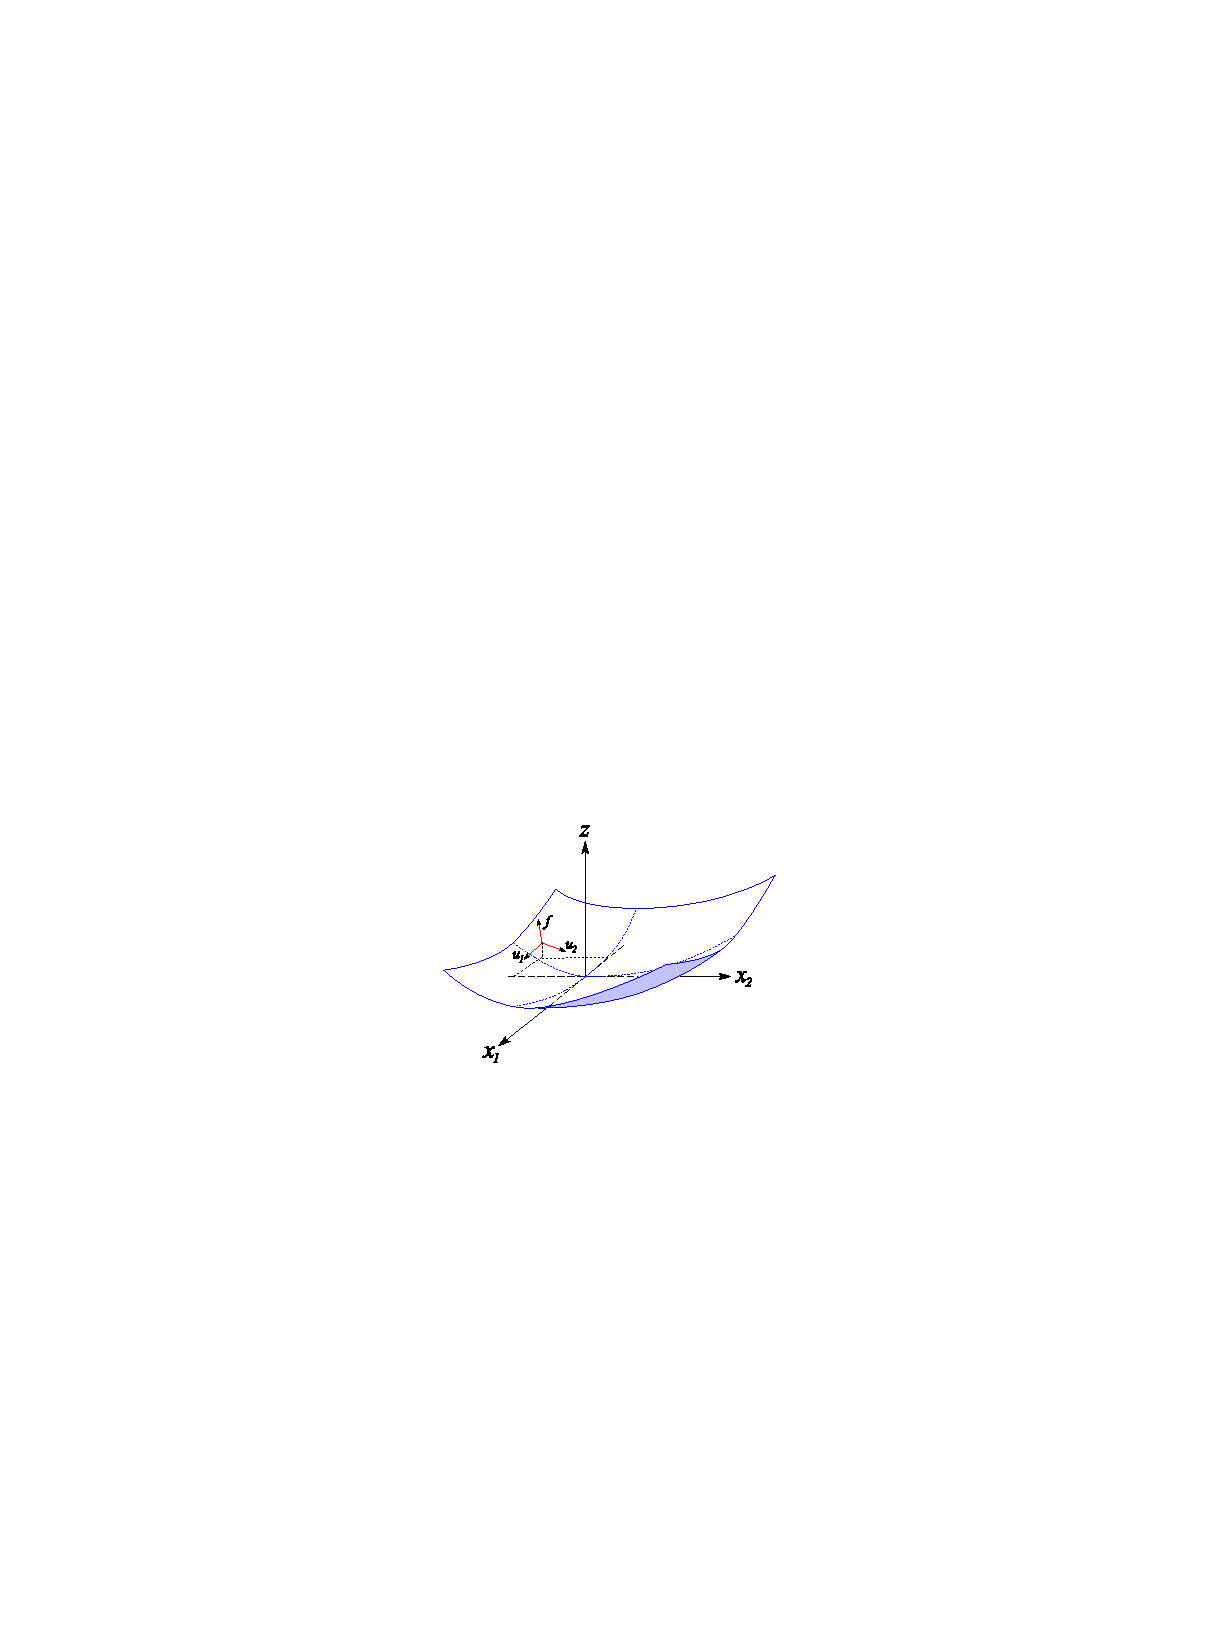
\includegraphics[width=4in]{nelsonS1}
\caption{
مبدا مختصات مماس به بخشی از کره‌ی بدون تغییر شکل.ٓ
}
\label{fig:nelson_figs1}
\end{center}
\end{figure}

که در اینجا 
$z=Z()z_1,x_2)$
نقاط روی کره در حالت بدون اختلال را مشخص می‌کند. در نظریه پوسته‌ی کم عمق فرض می‌شود که محل بررسی به اندازه‌ای کوچک است که شیب‌های 
$\partial_1Z\sim x_1/R$
و 
$\partial_2Z\sim x_2/R$
اندازه‌گیری شده نسبت به صفحه‌ی 
$(x_1,x_2)$
کوچک هستند. در نتیجه می‌توان معادله‌ی بالا رو به شکل زیر ساده کرد:
\begin{equation}
Z(x_1,x_2) \approx \frac{x_1^2+x_2^2}{2R}
\label{eq:nelsonS2}
\end{equation}
در نتیجه تمام تغییر شکل‌های پوسته از این حالت را می‌توان بر حسب جابجایی‌های عمود بر صفحه‌
 $f(x_1,x_2)$
و جابجایی های مماس بر صفحه 
$u_1(x_1,x_2)$
و
$u_2(x_1,x_2)$
که به ترتیب جابجایی در راستای محورهای 
$x_1$
و
$x_2$
را مشخص می‌کنند، تعریف کرد. بنابراین با توجه به میدان‌های تعریف شده، نقطه‌ی 
$(x_1,x_2,Z(x_1,x_2))$
در حالت بدون جابجایی در مرتبه‌ی اول به نقطه‌ی 
$(x_1+u_1-f\partial_1Z,x_2+u_2-f\partial_2Z,Z+f)$
منتقل می‌شود که در اینجا 
$\partial_iZ=x_i/R$
است. تانسور کرنش با توجه رابطه‌ی میان اندازه‌ی یک عنصر خط در حالت تغییر حالت داده شده
$ds'$
و خط متناظر آن در حالت کاملا کروی تعریف می‌شود:
\begin{equation}
(ds')^2=ds^2+2u_{ij}dx_idx_j
\label{eq:nelsonS3}
\end{equation}
در نتیجه با صرف نظر از مشتق‌های مرتبه‌های بالاتر می‌توان تانسور کرنش را تعریف کرد،
\begin{equation}
u_{ij}=\frac{1}{2}(\partial_iu_j+\partial_ju_i+\partial_if\partial_jf)-\delta_{ij}\frac{f}{R}
\label{eq:nelsonS4}
\end{equation}
در نتیجه انرژی کششی به شکل زیر تعریف خواهد شد
\begin{equation}
G_s=\frac{1}{2}\int dS\left[2\mu u_{ij}^2+\lambda u_{kk}^2\right]
\label{eq:nelsonS5}
\end{equation}
  که در اینجا 
$\lambda$
و
$\mu$
ضرایب لامه
\LTRfootnote{Lamé}
بوده و 
$dS$
عنصر مساحت است. همچنین انرژی هلفریش
\LTRfootnote{Helfrish}
را نیز در برای تغییرات خمشی پوسته در نظر می‌گیریم
\cite{Helfrich1973}.
\begin{equation}
G_b=\frac{1}{2}\int dS\left[\kappa(H-H_0)^2+\bar\kappa K\right]
\label{eq:nelsonS6}
\end{equation}
  که در اینجا 
$\kappa$
سختی خمشی، 
$H$
خمش متوسط (یا رد
\LTRfootnote{trace}
تانسور خمش)،
$H_0$
خمش ذاتی غشا،
$\bar\kappa$
مدول خمشی زینی،
و
$K$
دترمینان تانسور خمش است . با توجه به نظریه گاوس و بونه
\LTRfootnote{Gauss-Bonnet}
این انتگرال فقط یک عدد ثابت است که به انرژی آزاد سیستم اضافه می‌شود. در نتیجه از الان به بعد آن را در نظر نمی‌گیریم. همچنین فرض می‌کنیم که غشا خمش ذاتی ندارد. در نتیجه در قسمت کم عمق پوسته خمش موضعی بر حسب 
$Z(x_1,x_2)$
و 
$f(x_1,x_2)$
به شکل زیر محاسبه می‌شود:
\cite{Helfrich1973}.
\begin{equation}
H =\nabla^2(Z+f)=\frac{2}{R}+\nabla^2f
\label{eq:nelsonS7}
\end{equation}
که 
$\nabla^2=\partial_{11}+\partial_{22}$
لاپلاسین در دستگاه مختصات تعریف شده است. و در نهایت کار ناشی از فشار خارجی به صورت زیر تعریف می‌شود،
\cite{Helfrich1973}.
\begin{equation}
W=-p\int dSf
\label{eq:nelsonS8}
\end{equation}

و در نهایت  عنصر سطح به شکل زیر تعریف می‌شود،
\begin{equation}
dS=dx_1dx_2/\sqrt{1-(x_1^2+x_2^2)/R^2}\approx dx_1dx_2
\label{eq:nelsonS8.1}
\end{equation}
در نهایت با جمع کردن جملات انرژی کششی، خمشی، و فشار انرژی کشسانی سیستم به شکل زیر تغریف می‌شود:
\begin{equation}
G = G_s + G_b. + W =\int d^2x\left[\frac{\kappa}{2}(\nabla^2f)^2+\mu u_{ij}^2+\lambda u_{kk}^2-pf\right]
\label{eq:nelsonS8.2}
\end{equation}
همانطور که از نام این نظریه پیداست مدل بالا برای محاسبه‌ی انرژی لازم برای تغییر شکل‌ها کم عمق و کوچک است. مقیاس ما از اندازه‌ی کره شعاع آن
$R$
است. حد اندازه‌ی یک تغییر شکل کوچک را می‌توانیم با مقایسه‌ی انرژی کششی و خمشی محاسبه کنیم. انرژی کششی و خمشی برای قسمتی به اندازه‌ی
$\ell$
را با 
$G_s\sim Y(f/R)^2$
، که در اینجا $Y$ یک ثابت کششی‌ متداول است، و 
$G_b\sim\kappa f^2/\ell^4$
می‌توان تقریب زد. برابر قرار دادن این دو جمله، مقیاس طولی فوپل فون کارمان
\LTRfootnote{Föpplٓ-von Kármán}
را به ما می‌دهد
\begin{equation}
\ell^*=\frac{R}{\gamma^{1/4}}
\label{eq:nelsonS9}
\end{equation}
که در بالا عدد فوپل فون کارمان 
$\gamma=YR^2/\kappa$
است
\cite{nelsonPRE2003}
. با کمی محاسبه‌ی بیشتر می‌توان نشان داد که ثابت کششی که استفاده کردیم مدول ۲ بعدی یانگ است که برابر است با 
\begin{equation}
Y= \frac{4\mu(\mu+\lambda)}{2\mu+\lambda}
\label{eq:nelsonS9.1}
\end{equation}
با فرض داشتن یک پوسته‌ی کشسان با ضخامت $h$ و جایگذاری $\kappa$ و $Y$ با مدول ۳ بعدی یانگ برای یک ماده جامد همسان کشسان در نظریه پوسته‌ی کم عمق $\gamma\approx10(R/h)^2$ بدست می‌آید 
\cite{landau}
برای اینکه این نظریه پیشبینی درستی از مسئله داشته باشد نیاز است که $\ell^*\ll R$. پس این نظریه تنها زمانی که $\gamma\gg1$ یا $r\gg h$ باشد صادق است که این حد دقیقا متناظر با پوسته‌های نازکی است که می‌توانند تحت تاثیر بسیار زیاد افت و خیز ترمودینامیکی قرار بگیرند. کویتر
\LTRfootnote{Koiter}
در مطالعاتی نیز در مورد صحت پاسخ نظریه‌ی پوسته‌های کم عمق در مقایسه با نظریه‌های عمومی‌تر که می‌توان بر تمامی یک پوسته‌ی کشسان اعمال کرد را در حالتی که از دو نقطه‌ی قطبی به یک پوسته فشار وارد می‌شود بحث کرده است
\cite{koiter1963}
 . همچنین توسط هاتچینسون
\LTRfootnote{Hutchinson}
برای مطالعه‌ی پایداری پوسته‌های تحت فشار مطالعه شده‌است
\cite{Hutchinson1967}
. در هر دو مطالعه نشان داده شده که این نظریه در مقیاسی که در بالا محاسبه کردیم رفتار درستی از سیستم را نشان می‌دهد. از آنجایی که افت و خیز گرمایی روی پوسته‌هایی که شعاع آنها بسیار بزرگ‌تر از زخامتشان است تاثیر زیادی‌ می‌گذارد، این نظریه را می‌توان به عنوان نقطه‌ شروع توصیف این سیستم‌ها استفاده کرد.
\subsection{
از میان رفتن مُدهای فنونی درون صفحه‌ای و انقباض هماهنگ کروی بوسیله‌ی انتگرال گاووسی
}
\LTRfootnote{Elimination of in-Plane Phonon Modes and Uniform Spherical Contrac- tion by Gaussian Integration}
یک پوسته‌ی کروی تحت فشار هماهنگ خارجی که از حد مچاله شدن کره
\LTRfootnote{buckling}
کمتر است باعث می‌شود که کره در تمام نقاط به صورت هماهنگ به اندازه‌ی $f_0$ منقبض شود. در نتیجه‌ تغییر شکل‌های خارج از صفحه‌ای را می‌توان به صورت مجموع قسمت‌های هماهنگ و غیر هماهنگ نوشت،
\begin{equation}
f(\boldsymbol x)=f_0+f'(\boldsymbol x) = f_0+\sum_{\boldsymbol . q\neq0}f_{\boldsymbol q}e^{-i\boldsymbol q.\boldsymbol x}
\label{eq:nelsonS10}
\end{equation}
در اینجا $f'(\boldsymbol x)$ 
نماینده‌ی سهم میدان از مد‌های غیر صفر مولفه‌های فوریه‌ی آن است. در این بخش برای ساده سازی از نرمال کردن 
$f_{\boldsymbol q} \equiv \frac{1}{A}\int d^2xf(\boldsymbol x) e^{i\boldsymbol q.\boldsymbol x}$
استفاده شده که $A$ مساحت انتگرال گیری شده روی صفحه‌ی $(x_1,x_2)$ است. همچنین تبدیل واروون را نیز به شکل 
$f(\boldsymbol x) = \sum_{\boldsymbol q}f_{\boldsymbol q}e^{-i\boldsymbol q.\boldsymbol x}$
در این صورت 
$\int d^2xf'(\boldsymbol x)=0$
است و در نتیجه تنها جمله‌‌ی $f_0$ در محاسبه‌ی کار فشار باقی می‌ماند. از آنجایی که جمله‌ی $f'$ تنها در قسمت غیر خطی تانسور کرنش ظاهر می‌شود، پس انرژی کشسانی که در معادله‌ی \ref{eq:nelsonS8.2} تعریف شد در حالت انقباض تحت فشار هماهنگ $f_0$ و همچنین تحت جابجایی مُدهای درون صفحه‌ای $u_1(\boldsymbol x)$ و $u_2(\boldsymbol x)$ به شکل همسان
\LTRfootnote{harmonic}
 عمل می‌کند. برای بررسی رفتارهای غیر همسان بهتر است که این میدان‌ها را تقریب بزنیم و از انرژی آزاد مؤثر تعریف کنیم.
 \begin{equation}
G_{eff}=-k_BT\ln\left\{\int\mathcal D\vec u(x_1,x_2)\int df_0e^{-G[f',f_0,u_1,u_2]/k_BT}\right\}
\label{eq:nelsonS11}
\end{equation}
برای اینکه انتگرال تابعی را در معادله‌ی بالا را برای تعداد مشخصی میدان جابجایی خارج از صفحه‌ای $f'(\boldsymbol x)$ بتوانیم انجام دهیم باید جملات $\boldsymbol q = 0$ و $\boldsymbol q \neq 0$ تانسور کرنش $u_{ij}$ 
را نیز از هم جدا کنیم،

 \begin{equation}
u_{ij}=\tilde u_{ij}^0+\sum_{\boldsymbol q \neq 0}\left[\frac{i}{2}\left(q_iu_j(\boldsymbol q)+q_ju_i(\boldsymbol(q)\right)+A_{ij}(\boldsymbol q)-\delta{ij}\frac{f_{\boldsymbol q}}{R}\right]e^{-i\boldsymbol q.\boldsymbol x}
\label{eq:nelsonS12}
\end{equation}
که در بالا 
 \begin{equation}
A_{ij}(\boldsymbol q)=\frac{1}{2A}\int d^2x\partial_if'\partial_jf'e^{i\boldsymbol q.\boldsymbol x}
\label{eq:nelsonS13}
\end{equation}
قسمت هماهنگ تانسور کرنش از اجزای زیر تشکیل شده
\begin{equation}
\begin{aligned}
&\tilde u_{11}^0=u_{11}^0+A_{11}(\boldsymbol 0)-\frac{f_0}{R}, \\
&\tilde u_{22}^0=u_{22}^0+A_{22}(\boldsymbol 0)-\frac{f_0}{R}, \\
&\tilde u_{12}^0=u_{12}^0+A_{12}(\boldsymbol 0)
\label{eq:nelsonS14}
\end{aligned}
\end{equation}
در بالا $u_{ij}^0$ جملات کرنشی هماهنگ درون صفحه‌ای مستقل از $f_0$. این محدودیت باعث می‌شود که $u_{11}^0+u_{22}^0=0$ باشد زیرا اگر تغییر شکل هم علامت در راستای $x_1$ و $x_2$ در پوسته وجود داشته باشد به این معناست که شعاع پوسته در حال تغییر کردن است که تغییرات این چنین در  جمله‌ی $f_0$ در نظر گرفته شده است. در نتیجه علاوه بر $f_0$
و $u_{12}^0$
تنها یک درجه‌ی آزادی مستقل دیگر وجود دارد که در تانسور کرنش تاثیر هماهنگ دارد و آن $\Delta u^0 = u_{11}^0-u_{22}^0$ است.
در نهایت لازم است که انتگرال تابعی در معادله \ref{eq:nelsonS11} را روی میدان‌های فنونی $u_i$ 
و ۳ درجه‌ی آزادی مستقل که سهم جملات هماهنگ در تانسور کرنش دارند، 
$f_0$، $\tilde u_{12}^0$، و$\Delta u^0$
را حساب کنیم. پس از حذف جملاتی که به صورت عدد ثابل ظاهر می‌شوند انرژی آزاد مؤثر شکل زیر را به خود می‌‌گیرد،
ٓ\begin{equation}
G_{eff}=\int d^2x\left[\frac{\kappa}{2}(\nabla^2f')^2+\frac{Y}{2}\left(\frac{1}{2}P_{ij}^T\partial_if'\partial_jf'-\frac{f'}{R}\right)\right]-A\frac{pR}{2}[A_{11}(\boldsymbol 0)+A_{22}(\boldsymbol 0)]
\label{eq:nelsonS15}
\end{equation}
که در بالا $P_{ij}^T=\delta_{ij}-\partial_i\partial_j/\nabla^2$ عملگر تصویری عرضی‌ است
\LTRfootnote{transverse projection operator}
. توجه کنید که در نتیجه‌ی انتگرال گیری، مؤلفه‌های لامه $\mu$ و $\lambda$ فقط از طریق مدول ۲ بعدی یانگ وارد می‌شوند. در آخر با جایگذاری
\begin{equation}
A_{11}(\boldsymbol 0)+A_{22}(\boldsymbol 0)=\frac{1}{2A}\int d^2x\left[ (\partial_1f')^2+(\partial_2f')^2\right] = \frac{1}{2A}\int d^2x| \nabla f'|^2
\label{eq:nelsonS16}
\end{equation}
در معادله‌‌ی \ref{eq:nelsonS15} 
انرژی آزاد مؤثر $G_{eff}$ دو بخش هماهنگ $G_0$ 
و غیر هماهنگ $G_1$
خواهد داشت،
\begin{equation}
\begin{aligned}
&G_0=\frac{1}{2}\int d^2x\left[\kappa(\nabla^2f')^2-\frac{pR}{2}|\nabla f'|^2+\frac{Y}{R^2}f'^2\right], \\
&G_1=\frac{Y}{2}\int d^2x\left[\left(\frac{1}{2}P_{ij}^T\partial_if'\partial_jf'\right)^2-\frac{f'}{R}P_{ij}^T\partial_if'\partial_jf'\right],
\label{eq:nelsonS16.1}
\end{aligned}
\end{equation}
در معادله‌ی بالا $Y=4\mu(\mu+\lambda)/(2\mu+\lambda)$ مدول یانگ در ۲ بعد است. جمله‌ی «جرم» $Y(f'/R)^2$ در تابعی انرژی هماهنگ میزان جفت شدگی بین تغییر شکل خارج از صفحه و کشیدگیی که درون صفحه ایجاد می‌شود را مشخص می‌کند. این جمله در نظریه‌ی صفحات یا غشاهای تخت ظاهر نمی‌شود. همچنین برهمکنشی با ضریب $-Y/2R$ نیز جمله‌ایست که مخصوص غشاهای خمیده‌است و به علت وجود تقارن در غشاهای تخت دیده نمی‌شود. نکته جالب راجع به این جملات این است که در آنها پارامترهای وابسته به اندازه سیستم در آنها وجود دارد. توجه داشته باشید که برای فشارهای رو به داخل $p>0$ در قسمت هماهنگ معادله شبیه کشش سطحی منفی و وابسته به شعاع رفتار می‌کند. در حد $R\rightarrow \infty$ و $p=0$ انرژی غشای تخت بدست می‌آید. از آنجایی که $f_0$ 
پس از انتگرال گیری ظاهر نمی‌شود و از این پس به جای 
$f'$ از 
$f$ 
استفاده خواهیم کرد. اگر تنها اثر جملات هماهنگ را درنظر بگیریم، نتایج بر اساس اصل همپاری برای مؤلفه‌های فوریه ناشی از گرما برای موج ۲ بعدی

\begin{equation}
\begin{aligned}
&f_{\boldsymbol q} = \int d^2xf(\boldsymbol x)e^{i\boldsymbol q.\boldsymbol x}, \\
&\left\langle f_{\boldsymbol q}f_{\boldsymbol {q'}}\right\rangle_0 = \frac{Ak_BT\delta_{\boldsymbol q, \boldsymbol{-q'}}}{\kappa q^4-\frac{pR}{2}q^2+\frac{Y}{R^2}},
\label{eq:nelsonS17}
\end{aligned}
\end{equation}
که در بالا $A$
مساحت قسمت انتگرال گیری است. 
بزرگی طول موج‌ها بلند به علت اندازه محدود کره به $q\gtrsim 1/R$
محدود می‌شوند. برخلاف غشاهای تخت که طول موج‌های بلند $q\rightarrow 0$
با اهنگ $k_BT/(\kappa q^4)$
به بینهایت میل می‌کند، در غشاهای خمیده جفت شدگی میان خمیدگی خارج از صفحه و درون صفحه، طول موج افت و خیزها با سقف مشخصه‌ی طول سیستم محدود می‌شوند، 
\begin{equation}
q^*=(\ell^*)^{-1}=\left(\frac{Y}{\kappa R^2}\right)^{1/4}\equiv\frac{\gamma^{1/4}}{R}
\label{eq:nelsonS17.1}
\end{equation}
که ما در اینجا حالت‌های $\gamma\gg1$
که در نتیجه $\ell^*\ll R$
را بررسی می‌کنیم. در حالی که $p$
به $p_c\equiv4\sqrt{\kappa Y}/R^2$
نزدیک می‌شود،. طول موج‌های $q=q^*$ 
ناپایدار شده و اندازه‌ی آنها به بی‌نهایت می‌رود. در نتیجه این حالت معادل با مچاله شدن پوسته‌ی کروی تحت فشارهای خارجی بالاتر از حد تحمل سیستم است. برای فشارهای بیشتر از $p_c$
نمی‌توانیم از این نظریه استفاده کنیم زیرا که تغییرات در شکل کره فراتر از تغییرات کم عمق خواهد بود.

معادله‌ی \ref{eq:nelsonS17}
 رفتار هماهنگ پوسته‌ی کروی را بیان می‌کند، برای بررسی رفتار ناهماهنگ پوسته نیاز است که به این معادله جمله‌های تصحیح کننده اضافه کنیم.
 \subsection{محاسبه‌ی سهم تک حلقه در خود انرژی}
 \begin{figure}[h]
\begin{center}
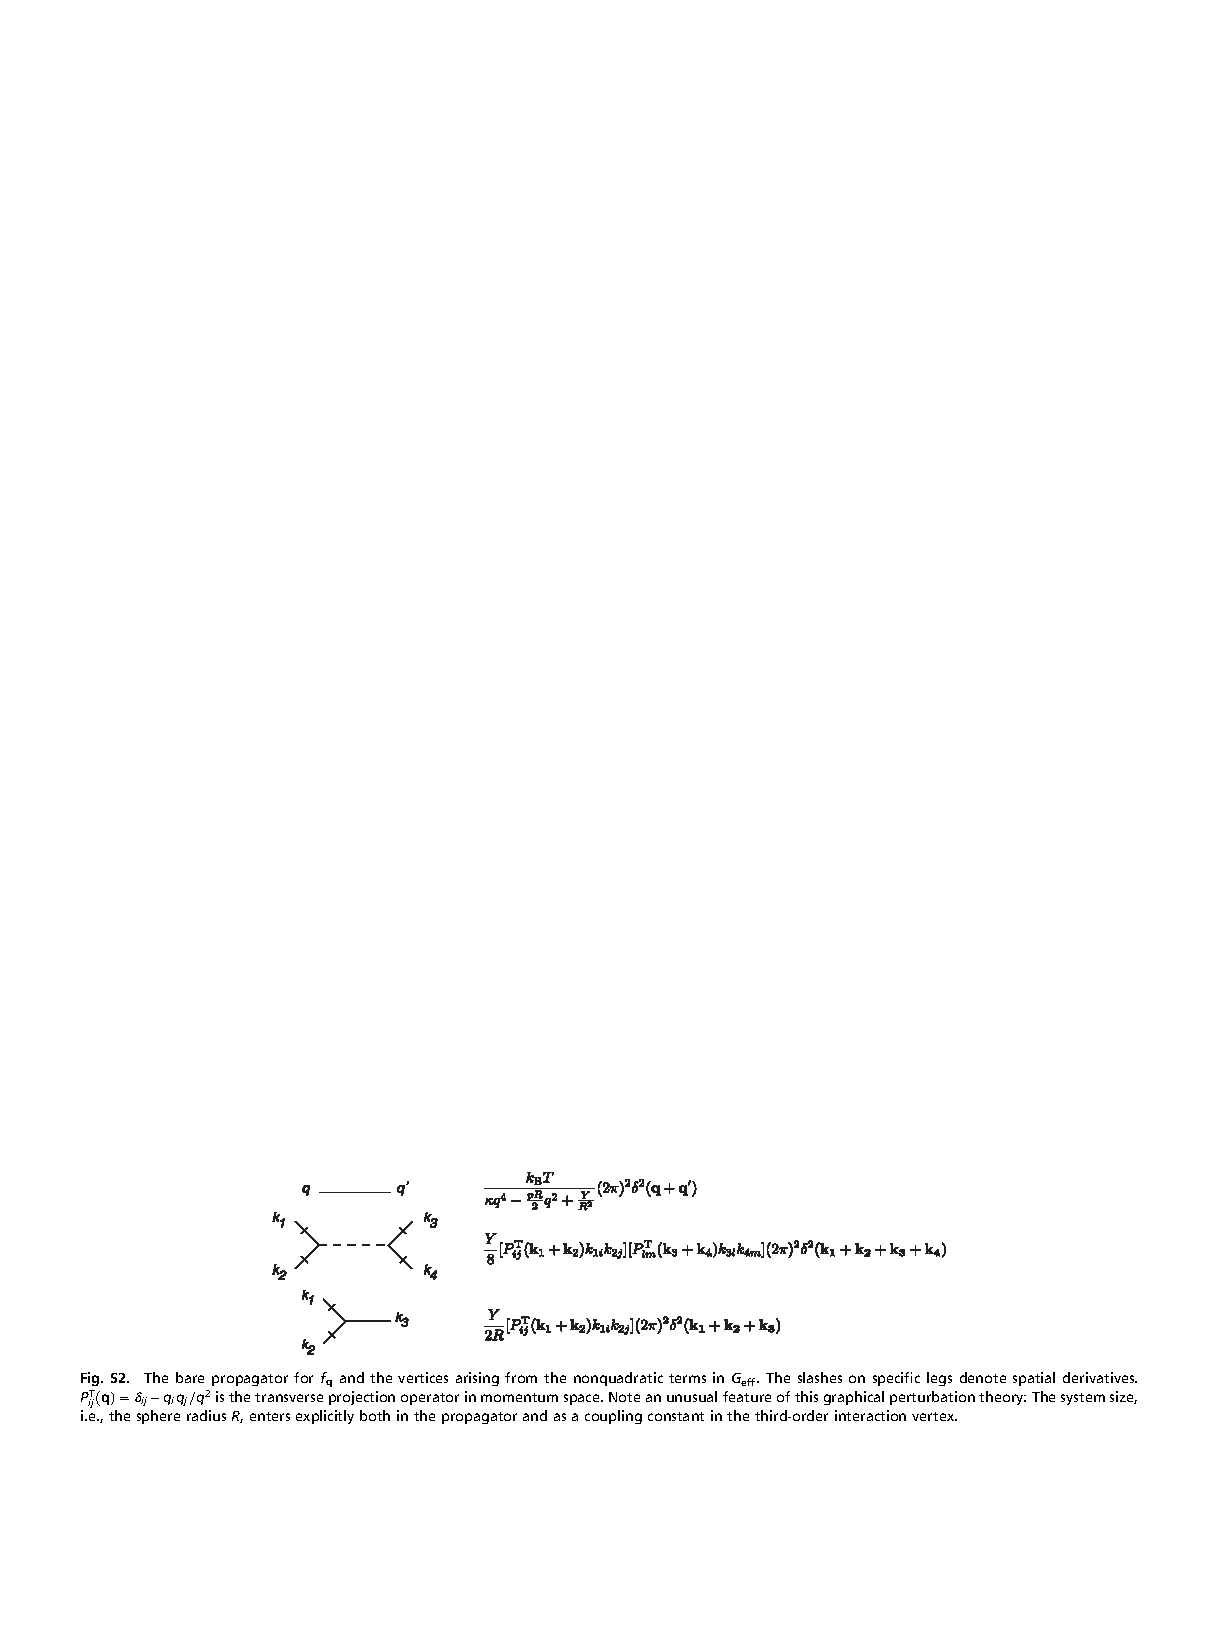
\includegraphics[width=4in]{nelsonS2}
\caption{
غشا با هندسه‌ی کروی.
}
\label{fig:nelsonS2}
\end{center}
\end{figure}

\begin{figure}[h]
\begin{center}
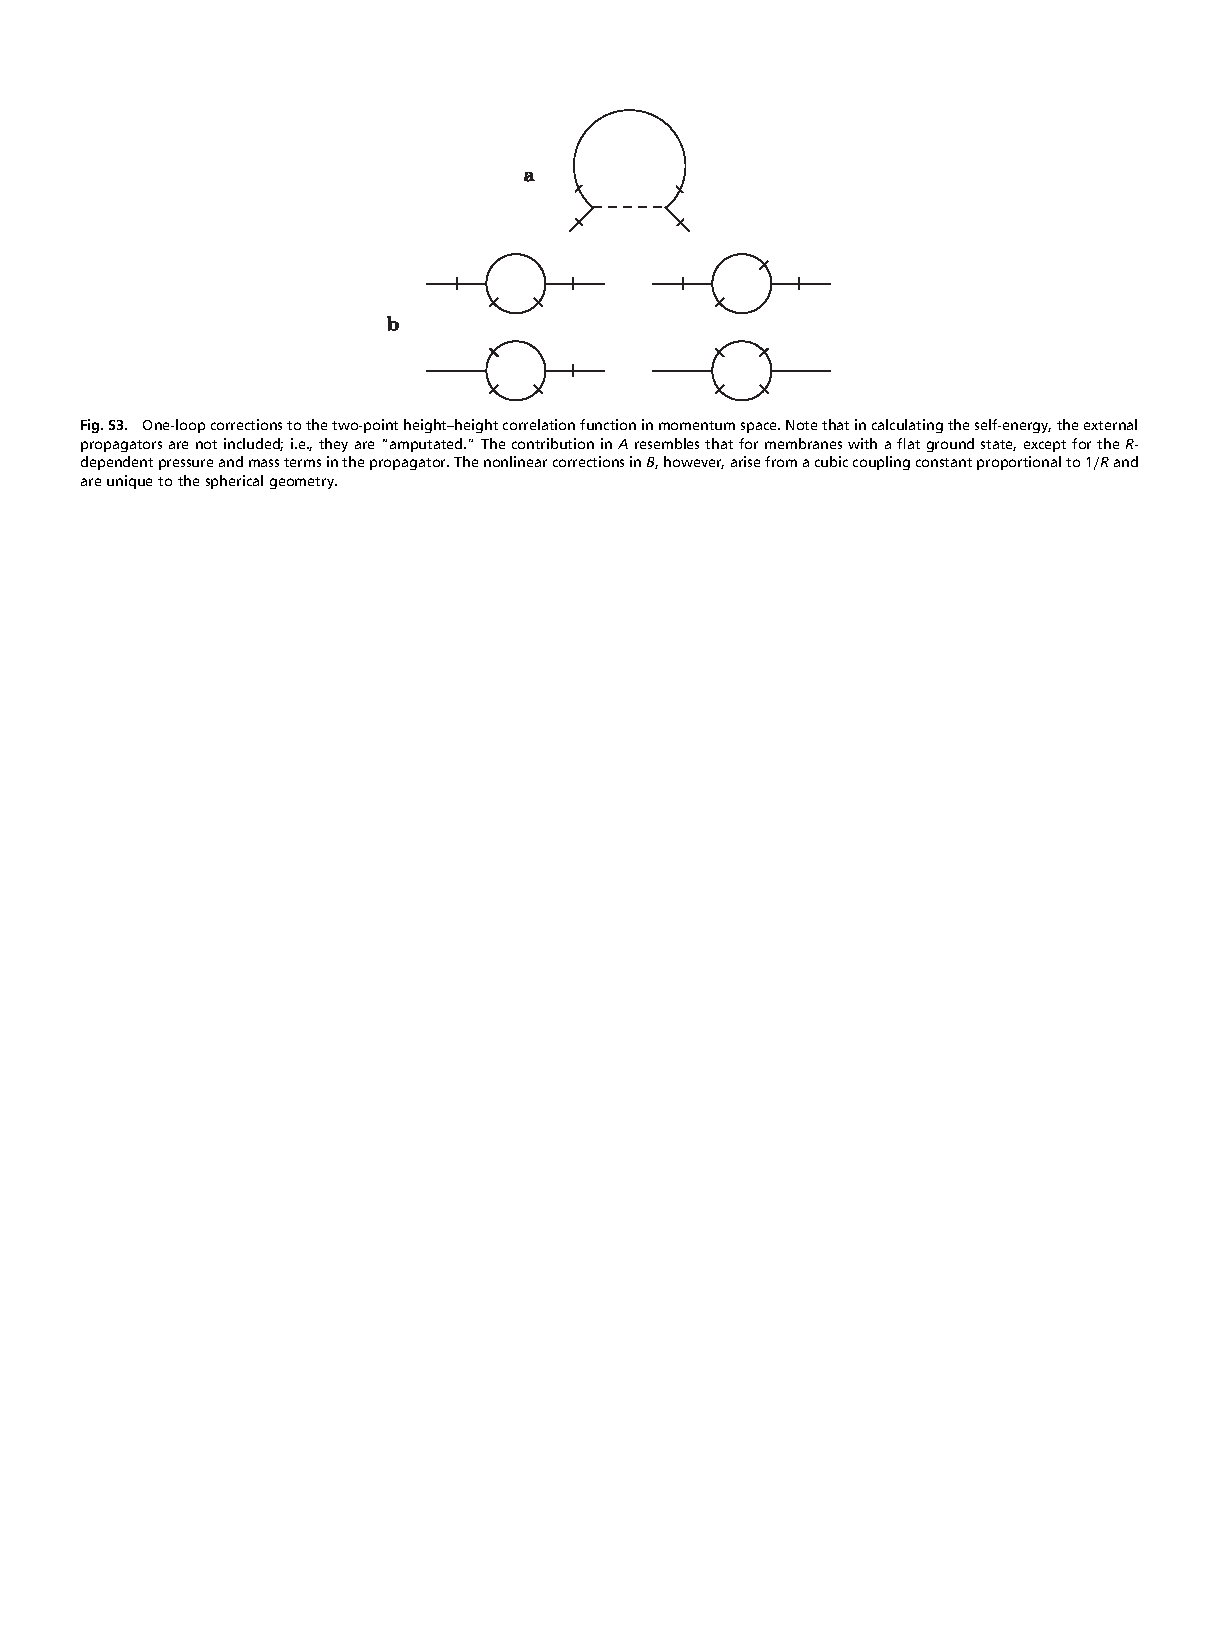
\includegraphics[width=4in]{nelsonS3}
\caption{
غشا با هندسه‌ی کروی.
}
\label{fig:nelsonS3}
\end{center}
\end{figure}
X
 قوانین فاینمن برای برگرفته شده از معادله‌ی \ref{eq:nelsonS15} 
 در شکل \ref{fig:nelsonS2}
 خلاصه شده است. از این پس مؤلفه‌های تبدیل فوریه به شکل
 $f_{\boldsymbol q}=\int d^2xf(\boldsymbol x)\exp(i\boldsymbol q.\boldsymbol x)$
 تعریف می‌شود. تبدیل فوریه‌ی وارون تغییر شکل‌های خارج از صفحه نیز به صورت
\begin{equation}
f(\boldsymbol x)=\frac{1}{A}\sum_{\boldsymbol q\neq 0}f_{\boldsymbol q}e^{-i\boldsymbol q.\boldsymbol x}
\label{eq:nelsonSٓ18}
\end{equation}
تعریف می‌شود و جمع روی تمام طول موج‌های مجاز است. خود انرژی ناشی از جمله‌ی ناهماهنگ ۳ نقطه‌ای و ۴ نقطه‌ای در شکل \ref{fig:nelsonS3}
الف خلاصه شده‌اند و این جملات برای توصیف غشای تخت نیز لازم هستند و به شکل 
\begin{equation}
-Y\int\frac{d^2k}{(2\pi)^2}\frac{\left[P_{ij}^Tq_iq_j\right]^2}{\kappa|\boldsymbol q + \boldsymbol k|^4-\frac{pR}{2}|\boldsymbol q + \boldsymbol k|^2+\frac{Y}{R^2}}
\label{eq:nelsonS19}
\end{equation}
 مجموع جملات خود انرژی ناشی از نمودارهای \ref{fig:nelsonS3}
 ب،

\begin{equation}
\begin{aligned}
&\frac{Y^2}{R^2} \int\frac{d^2k}{(2\pi)^2} \frac{1}{ 
\left( \kappa|\boldsymbol q + \boldsymbol k|^4 - \frac{pR}{2} |\boldsymbol q + \boldsymbol k|^2 + \frac{Y}{R^2} \right)
\left( \kappa k^4 - \frac{pR}{2}k^2 + \frac{Y}{R^2} \right) 
} \\
&\times\left\{ 
\frac{1}{2} \left[ P_{ij}^T(\boldsymbol q)k_ik_j\right]^2 + 
\left[P_{ij}^T(\boldsymbol k)q_iq_j\right]^2 + 
\left[P_{ij}^T(\boldsymbol k)q_iq_j\right] 
\left[P_{lm}^T(\boldsymbol{k+ q})q_lq_m\right] \right.\\
& \left.+ 2\left[P_{ij}^T(\boldsymbol k)q_iq_j\right]
\left[P_{lm}^T(\boldsymbol{q})k_lk_m\right]
\right\}
\label{eq:nelsonS20}
\end{aligned}
\end{equation}
وارون تابع همبستگی هماهنگ که در معادله‌ی \ref{eq:nelsonS17} مشاهده کردید فقط از جملات $q^0$، $q^2$، و $q^4$ تشکیل شده است و تصحیحات تک حلقه (که در معادلات \ref{eq:nelsonS19} و \ref{eq:nelsonS20} محاسبه شد) انجام شده به طیف جملاتی با همین توان‌ها و همچنین جملاتی با مرتبه‌ی $q^6$ نیز اضافه می‌کند. اگر  تصحیحات را تنها تا مرتبه‌ی $q^4$ نگه داریم می‌توانیم طیف را برای $q$های
کوچک تقریب بزنیم. 
\begin{equation}
Ak_BT\left\langle|f_{\boldsymbol q\rightarrow \boldsymbol 0}|^2\right\rangle^{-1} \equiv\kappa_Rq^4-\frac{p_RR}{2}q^2+\frac{Y_R}{R^2}+O(q^6)
\label{eq:nelsonS21}
\end{equation}
 که در بالا $Y_R$، $\kappa_R$، و $p_R$ به ترتیب مدول یانگ مؤثر، سختی خمش مؤثر، و فشار بی بعد. در مقیاس‌های طولی بزرگ اندازه‌گیری مشخصات کشسانی پوسته‌هایی که با گرما افت و خیز می‌کنند اطلاعاتی در مورد مشخصات مؤثر کشسانی در اختیار ما قرار می‌دهد. استفاده از این مشخصات بهتر از استفاده از مدول‌های خام $Y$، $\kappa$، و $p$
است که با تقریب دمای صفر رفتار پوسته در دما توصیف می‌کنند. با استفاده از معادلات \ref{eq:nelsonS19} و \ref{eq:nelsonS20} 
تا مرتبه‌ی $O(q^4)$
می‌توان انتگرال‌های تکانه را برای خود انرژی محاسبه کنیم،
\begin{equation}
Y_R=Y\left[1-\frac{3}{128\pi}\frac{k_BT}{\kappa}\frac{\sqrt\gamma}{(1-\eta^2)^{3/2}}\left(\eta\sqrt{1-\eta^2}+\pi-\cos^{-1}\eta\right)\right]
\label{eq:nelsonS22}
\end{equation}

\begin{equation}
\begin{aligned}
&\kappa_R=\kappa\left[1+\frac{1}{30720\pi}\frac{k_BT}{\kappa}\frac{\sqrt\gamma}{(1-\eta^2)^{7/2}}\right.\\
&\left.\left[\times\eta\sqrt{1-\eta^2}(-1699+3758\eta^2-2104\eta^4) \right.\right.\\
& \left.\left. +15(61-288\eta^2+416\eta^4-192\eta^6)(\pi-\cos^{-1}\eta)\right]\right]
\label{eq:nelsonS23}
\end{aligned}
\end{equation}

\begin{equation}
\begin{aligned}
&\eta_R=\eta+\frac{1}{1536\pi}\frac{k_BT}{\kappa}\frac{\sqrt\gamma}{(1-\eta^2)^{5/2}}\\
&\times\left[\sqrt{1-\eta^2}(64-67\eta^2)+3(21\eta-22\eta^3)(\pi-\cos^{-1}\eta)\right]
\label{eq:nelsonS24}
\end{aligned}
\end{equation} 
و در معادلات بالا فشار بی بعد $\eta=p/p_c$
تعریف کردیم. به طور مشخص زمانی که $\eta\rightarrow1$
این کمیت‌ها به بی‌نهایت میل می‌کنند. این جملات برای پایین‌ترین مرتبه فشار خارجی به شکل زیر تقریب زده می‌شوند،
 \begin{equation}
Y_R\approx Y\left[1-\frac{3}{256}\frac{k_BT}{\kappa}\sqrt\gamma\left(1+\frac{4}{\pi}\frac{p}{p_c}\right)\right]
\label{eq:nelsonS25}
\end{equation}

\begin{equation}
p_R\approx p+\frac{1}{24}\frac{k_BT}{\kappa}p_c\sqrt\gamma\left(1+\frac{63\pi}{128}\frac{p}{p_c}\right)
\label{eq:nelsonS26}
\end{equation}

\begin{equation}
\kappa_R\approx \kappa\left[1+\frac{61}{4096}\frac{k_BT}{\kappa}\sqrt\gamma\left(1-\frac{1568}{915\pi}\frac{p}{p_c}\right)\right]
\label{eq:nelsonS27}
\end{equation}
برای محاسبه‌ی انتگرال‌های بالا باید از انتگرال‌های معادلات \ref{eq:nelsonS19} و \ref{eq:nelsonS20} روی تمام طول‌ موج‌های مجاز فضای فاز انتگرال بگیریم. طول‌ موج‌ها از حد پایین $k_{min}\sim1/R$ تا حد بالای طول موج‌ که با ثابت میکروسکوپیک شبکه‌ی شبکه تعیین می‌شود، است. از آنجایی که تمام انتگرال‌ها در حد بالا به حد فرابنفش همگرا می‌شوند می‌ توانیم $k\rightarrow\infty$. به علت وجود جمله‌ی «جرم» $\sim Y/R^2$ انتگرال در محدوده‌ی طول موج‌های کوچک خوش رفتار است، و در نتیجه می‌توان انتگرال را در این محدوده روی تمام فضای فاز دو بعدی انجام دهیم. اینکه انتگرال را برای محدوده‌ی پایین‌تر از فروسرخ یا $0<k<1/R$ انجام دهیم باعث ایجاد خطای از مرتبه‌ی $1/\sqrt\gamma$ می‌شود که برای پوسته‌های خیلی نازک قابل صرف نظر کردن است. 

با نگاه کردن به معادلات $\ref{eq:nelsonS25}، $\ref{eq:nelsonS26}، و \ref{eq:nelsonS27} می‌بینیم که در حد طول موج‌های بلند تغییر شکل‌های تابع مدول یانگ موثر کوچکتر، سختی خمش مؤثر بزرگتر، و کشش سطحی غیر صفر منفی است. این رفتار حتی وقتی که فشار خارجی صفر باشد نیز صادق است. وقتی $p/p_c$ بزرگ باشد، مدول یانگ و سختی خمش از تقریب دمای صفر کوچکتر می‌شوند و اندازه‌ی کشش سطحی مؤثر منفی که با $p_c$ تعیین می‌شود بسیار بزرگ می‌شود. محاسبات خطاهای مرتبه‌های بالاتر همگی نشان می‌دهند که با $p/p_c\rightarrow1$ تمام تصحیحات به بی‌نهایت میل می‌کنند. همچنین مشا‌هده می‌کنیم که تمام مشخصات مؤثر تابع دما و اندازه‌ی سیستم هستند زیرا که $\sqrt\gamma\sim R$ . با اینکه برای $k_BT\ll\kappa$ 
سهم تصحیحات ناچیز است ولی باید در نظر بگیریم که با بزرگ شدن شعاع سیستم $R\rightarrow\infty$ 
به بینهایت میل می‌کند. 


کشش سطحی ناشی از افت و خیز گرمایی و تابعیت قوی آن با فشار خارجی، همچنین تابعید ثابت کشسانی سیستم با اندازه‌ی سیستم مشخصات مختص غشاهای کروی است و در غشا‌های تخت دیده نمی‌شود. 
\subsection{بررسی با استفاده از هماهنگ‌های کروی}
یک پوسته‌ی کروی با شعاع $R$، سختی خمش $\kappa$ و مؤلفه‌های لامه $\mu$ و $\lambda$ 
در نظر بگیرید که تحت یک میدان مماسی $\boldsymbol u(u_x,u_y)$
و میدان جابجایی شعاعی $f$
قرار گرفته‌است. میدان $\boldsymbol u$
را مانند تمام میدان‌های خوش رفتار می‌توان مجموع یک بخش بدون چرخش
\LTRfootnote{curl free}
و بخش بدون واگرایی
\LTRfootnote{divergence free}
نوشت، $\boldsymbol u\equiv\nabla\boldsymbol\Psi+\boldsymbol v$ که تابع اسکالر $\boldsymbol\Psi$ قسمت غیرچرخش
\LTRfootnote{irrotational}
 را تولید می‌کند و $\boldsymbol v$ بخش مارپیچی
 \LTRfootnote{solenoidal}
 است. در بخش شعاعی مختصات شعاعی نود $i$ 
 در مختصات زاویه‌ای $(\theta,\phi)$ را می‌توانیم به شکل $r_i(\theta,\phi)=R_0+f(\theta,\phi)$
 نوشت و $R_0$ در اینجا شعاع متوسط کره‌ی در حال افت و خیز است.
 هنگام بسط دادن بر حسب هماهنگ‌ها کروی حقیقی به شکل
\begin{equation}
\begin{aligned}
&f(\theta,\phi)=R\sum_{l=0}^{l_M}\sum_{m=-l}^{m=l}A_{lm}Y_{lm}(\theta,\phi)\\
&\boldsymbol\Psi(\theta,\phi)=R^2\sum_{l=0}^{l_M}\sum_{m=-l}^{m=l}B_{lm}Y_l^m(\theta,\phi)
\label{eq:nelsonS28.1}
\end{aligned}
\end{equation} 

خواهند بود و انرژی کشسانی تغییر شکل آن تا مرتبه‌ی دوم تحت این میدان‌ها طبق معادله‌ی زیر خواهد بود \cite{krollPRE1993}

\begin{equation}
\begin{aligned}
&G=R^2\sum_{l,m}\left\{\left[\frac{\kappa}{2}\frac{(l+2)^2(l-1)^2}{R^2}+2K\right]A_{lm}^2-2Kl(l+1)A_{lm}B_lm\right.\\
&\left.+\frac{1}{2}l(l+1)[(K+\mu)l(l+1)-2\mu]B_{lm}^2\right\}+G_{sol}(\boldsymbol v)
\label{eq:nelsonS28}
\end{aligned}
\end{equation} 
که در اینجا $K=\mu+\lambda$
برابر مدول حجمی‌ 
\LTRfootnote{bulk modulus}
است. قسمت مارپیچی باعث انرژی در جابجایی شعاعی نشده و انرژی جداگانه با تابعیت $\boldsymbol v$ با تابعیت مربعی دارد. همچنین به معادله‌ی بالا انرژی ناشی از کشش سطحی منفی $-pR/2$ که در اثر انقباض ناشی از وجود فشار خارجی بوجود می‌آید را به صورت $G_s=-(pR/2)\Delta A$ اضافه می‌کنیم. در اینجا $\Delta A$ سطحی مضاعفی است که به علت تغییر شکل نسبت به شعاع میانگین ایجاد می‌شود. می‌توان میزان سطح مضاعف را بر حسب هماهنگ‌های کروی نوشت.
\cite{milnersafranPRA1987}
\begin{equation}
\Delta A\approx R^2\sum_{l>1,m}A_{lm}^2\left[1+\frac{l(l+1)}{2}\right]
\label{eq:nelsonS29}
\end{equation} 
همانند تقریب انرژی کشسانی پوسته‌های کم عمق اینجا نیز روی جملات مرتبه‌ی دوم $B_{lm}$ و $\boldsymbol v$ انتگرال می‌گیریم و انرژی آزاد مؤثر سیستم را بر حسب جابجایی شعاعی می‌نوسیم،
\begin{equation}
\begin{aligned}
&G_{eff}=\frac{R^2}{2}\sum_{l>1,m}\left\{\frac{\kappa(l+2)^2(l-1)^2}{R^2}-pR\left[1+\frac{l(l+1)}{2}\right]\right.\\
&\left.+\frac{4\mu(\mu+\lambda)(l^2+l-2)}{(2\mu+\lambda)(l^2+l)-2\mu}\right\}A_{lm}^2
\label{eq:nelsonS30}
\end{aligned}
\end{equation} 
 با توجه به نظریه هم پاری انرژی،
\begin{equation}
\begin{aligned}
&k_BT\left\langle|A_{lm}|^2\right\rangle_0^{-1}\\
&=\kappa(l+2)^2(l-1)^2-pR^3\left[1+\frac{l(l+1)}{2}\right]+\frac{4\mu(\mu+\lambda)(l^2+l+2)}{(2\mu+\lambda)(l^2+l)-2\mu}R^2\\
&=\kappa(l+2)^2(l-1)^2-pR^3\left[1+\frac{l(l+1)}{2}\right]+\frac{Y}{1+\frac{Y}{2\mu(l^2+l-2)}}R^2
\label{eq:nelsonS31}
\end{aligned}
\end{equation} 
که $Y$ مدول یانگ ۲ بعدی است که قبل‌تر تعریف کردیم. حالا می‌توانیم با استفاده از پارامتر‌های وابسته به دمای مؤثر $Y_R$، $\kappa_R$، و $p_R$ به جای پارامتر‌های پایه‌ای تغییرات در افت خیز ناشی از گرما را تعریف کرد. ولی برای محاسبه‌ی آخرین جمله در معادله‌ی \ref{eq:nelsonS31} 
نیاز داریم تصحیحات گرمایی وارد بر مؤلفه‌های لامه $\mu$
و $\lambda$ 
را بدانیم. در محاسبات مربوط به نظریه‌ی پوسته‌های کم عمق این مؤلفه‌ها در محاسبات نهایی حذف شدند. در شبیه‌سازی که در مطالعه‌ی 
\cite{gomppernelson2012}
برای انرژی کشسانی گسسته‌سازی شده $\mu=3Y/8$
محاسبه شده. اگر فرض کنیم که تصحیحات گرمایی ناشی از مرتبه‌ی تک حلقه ناچیز است می‌توانیم فرض کنیم که $Y_R\approx Y$ 
است. با جایگذاری در معدله‌ی \ref{eq:nelsonS31} به همراه پارمتر‌های مؤثر دیگر به شکل نهایی زیر می‌رسیم،
\begin{equation}
\begin{aligned}
&k_BT\left\langle|A_{lm}|^2\right\rangle^{-1}\\
&\approx\kappa_R(l+2)^2(l-1)^2-p_RR^3\left[1+\frac{l(l+1)}{2}\right]+Y_RR^2\left[\frac{3(l^2+l-2)}{3(l^2+l)-2}\right]
\label{eq:nelsonS32}
\end{aligned}
\end{equation} 
حتی اگر تصحیحات گرمایی وارد بر $\mu$
و $Y$
از مرتبه‌ی $O(k_BT)$ 
باشد می‌توان اختلاف خطای اضافه شده هنگامی که فرض کردیم $\mu_R\approx3Y_R/8$
حد بالای 
$4[3(l^2+l-2)+4]$
نسبت به تغییرات ناهماهنگ دارد و در نتیجه هنگامی که $l>1$
یک مرتبه‌ی بزرگی کوچکتر خواهد بود.


%\renewcommand{\refname}{whatever}
%\bibliography{reference} 
%\bibliographystyle{IEEEtran}
%\renewcommand\refname{مراجع}


	        
	       

\unsetRL
\bibliography{reference} 

\bibliographystyle{IEEEtran}
%\renewcommand{\contentsname}{whatever}
%\renewcommand{\refname}{whatever}
%\renewcommand\refname{مراجع}

%\printbibliography[title={Reference}]

\end{document}